\documentclass[12pt,a4paper]{article}
\usepackage[utf8]{inputenc}
\usepackage[czech]{babel}
\usepackage{datetime}
\usepackage{tabularx}
\usepackage{graphicx}
\usepackage{float}
\usepackage[colorlinks=true,linkcolor=blue,urlcolor=green]{hyperref}
\renewcommand{\dateseparator}{. }
\begin{document}

\title{Experimentální hodnocení kvality algoritmů}
\author{Dominik Plíšek}
\date{\dmyyyydate\today}
\maketitle

\tableofcontents


\section*{Úvod}

Zadáním této úlohy je zkoumat citlivost připravených algoritmů pro řešení 0/1 problému batohu na změnách některých parametrů instancí. Rozhodl jsem se citlivost zkoumat tak, že jsem zafixoval všechny parametry na rozumných hodnotách, a pak v každé následující sekci iterativně měnil jeden z nich. Pro každý algoritmus jsem pozoroval čas výpočtu, a speciálně u heuristického algoritmu založeném na poměru ceny a váhy, který je aproximativní, jsem pozoroval i vývoj relativní chyby. 

Základní nastavení parametrů, které jsem zvolil, je následující:

\begin{verbatim}
numThings=9
numInsts=50
ratio=0.5       # capacity to total weight
exp=1           # 1/w^exp for small things or 1/(wmax-w)^exp for big things
balance=0       # -1 for small things or 1 for big things
maxCost=100
maxWeight=100
\end{verbatim}

Věcí, které je třeba do batohu umístit, není příliš mnoho, aby netrvalo příliš dlouho vyřešit problém hrubou silou, ale zároveň jich není příliš málo, aby byl stavový prostor dostatečně velký.

Instancí je padesát, to znamená, že každé jednotlivé měření je prováděno na 50 vygenerovaných vlastností daných parametrů, aby bylo možné pozorovat dostatečně obecnou závislost na parametrech.

Výchozí poměr kapacity ku celkové váze věcí je 0.5, to znamená, že se vejde řádově půlka věcí.

Ve výchozím stavu není žádné přiklánění k těžším ani lehčím předmětům (balance=0). Nejvyšší cenu i váhu jsem zafixoval na 100.






\section{Změna maximální váhy}
\label{maxWeight}

Jedním z nastavitelných parametrů instancí je maximální váha, kterou může předmět batohu dosáhnout. Tento parametr jsem zvolil měnit od nejmenší hodnoty 10 po nejvyšší 100. Tím jsem získal 91 různých měření, každé provedené na 50 vygenerovaných instancích daných vlastností. Tyto jsem mezi sebou srovnával pomocí grafů.

Graf pro řešení hrubou silou je zobrazen na obrázku \ref{maxWeight/BruteForce}. Výpočetní čas se pohybuje kolem 2 milisekund, ale jeho rozložení v rozsahu maximální váhy 10 až 100 se zdá být lineární.

\begin{figure}[H]
\begin{center}
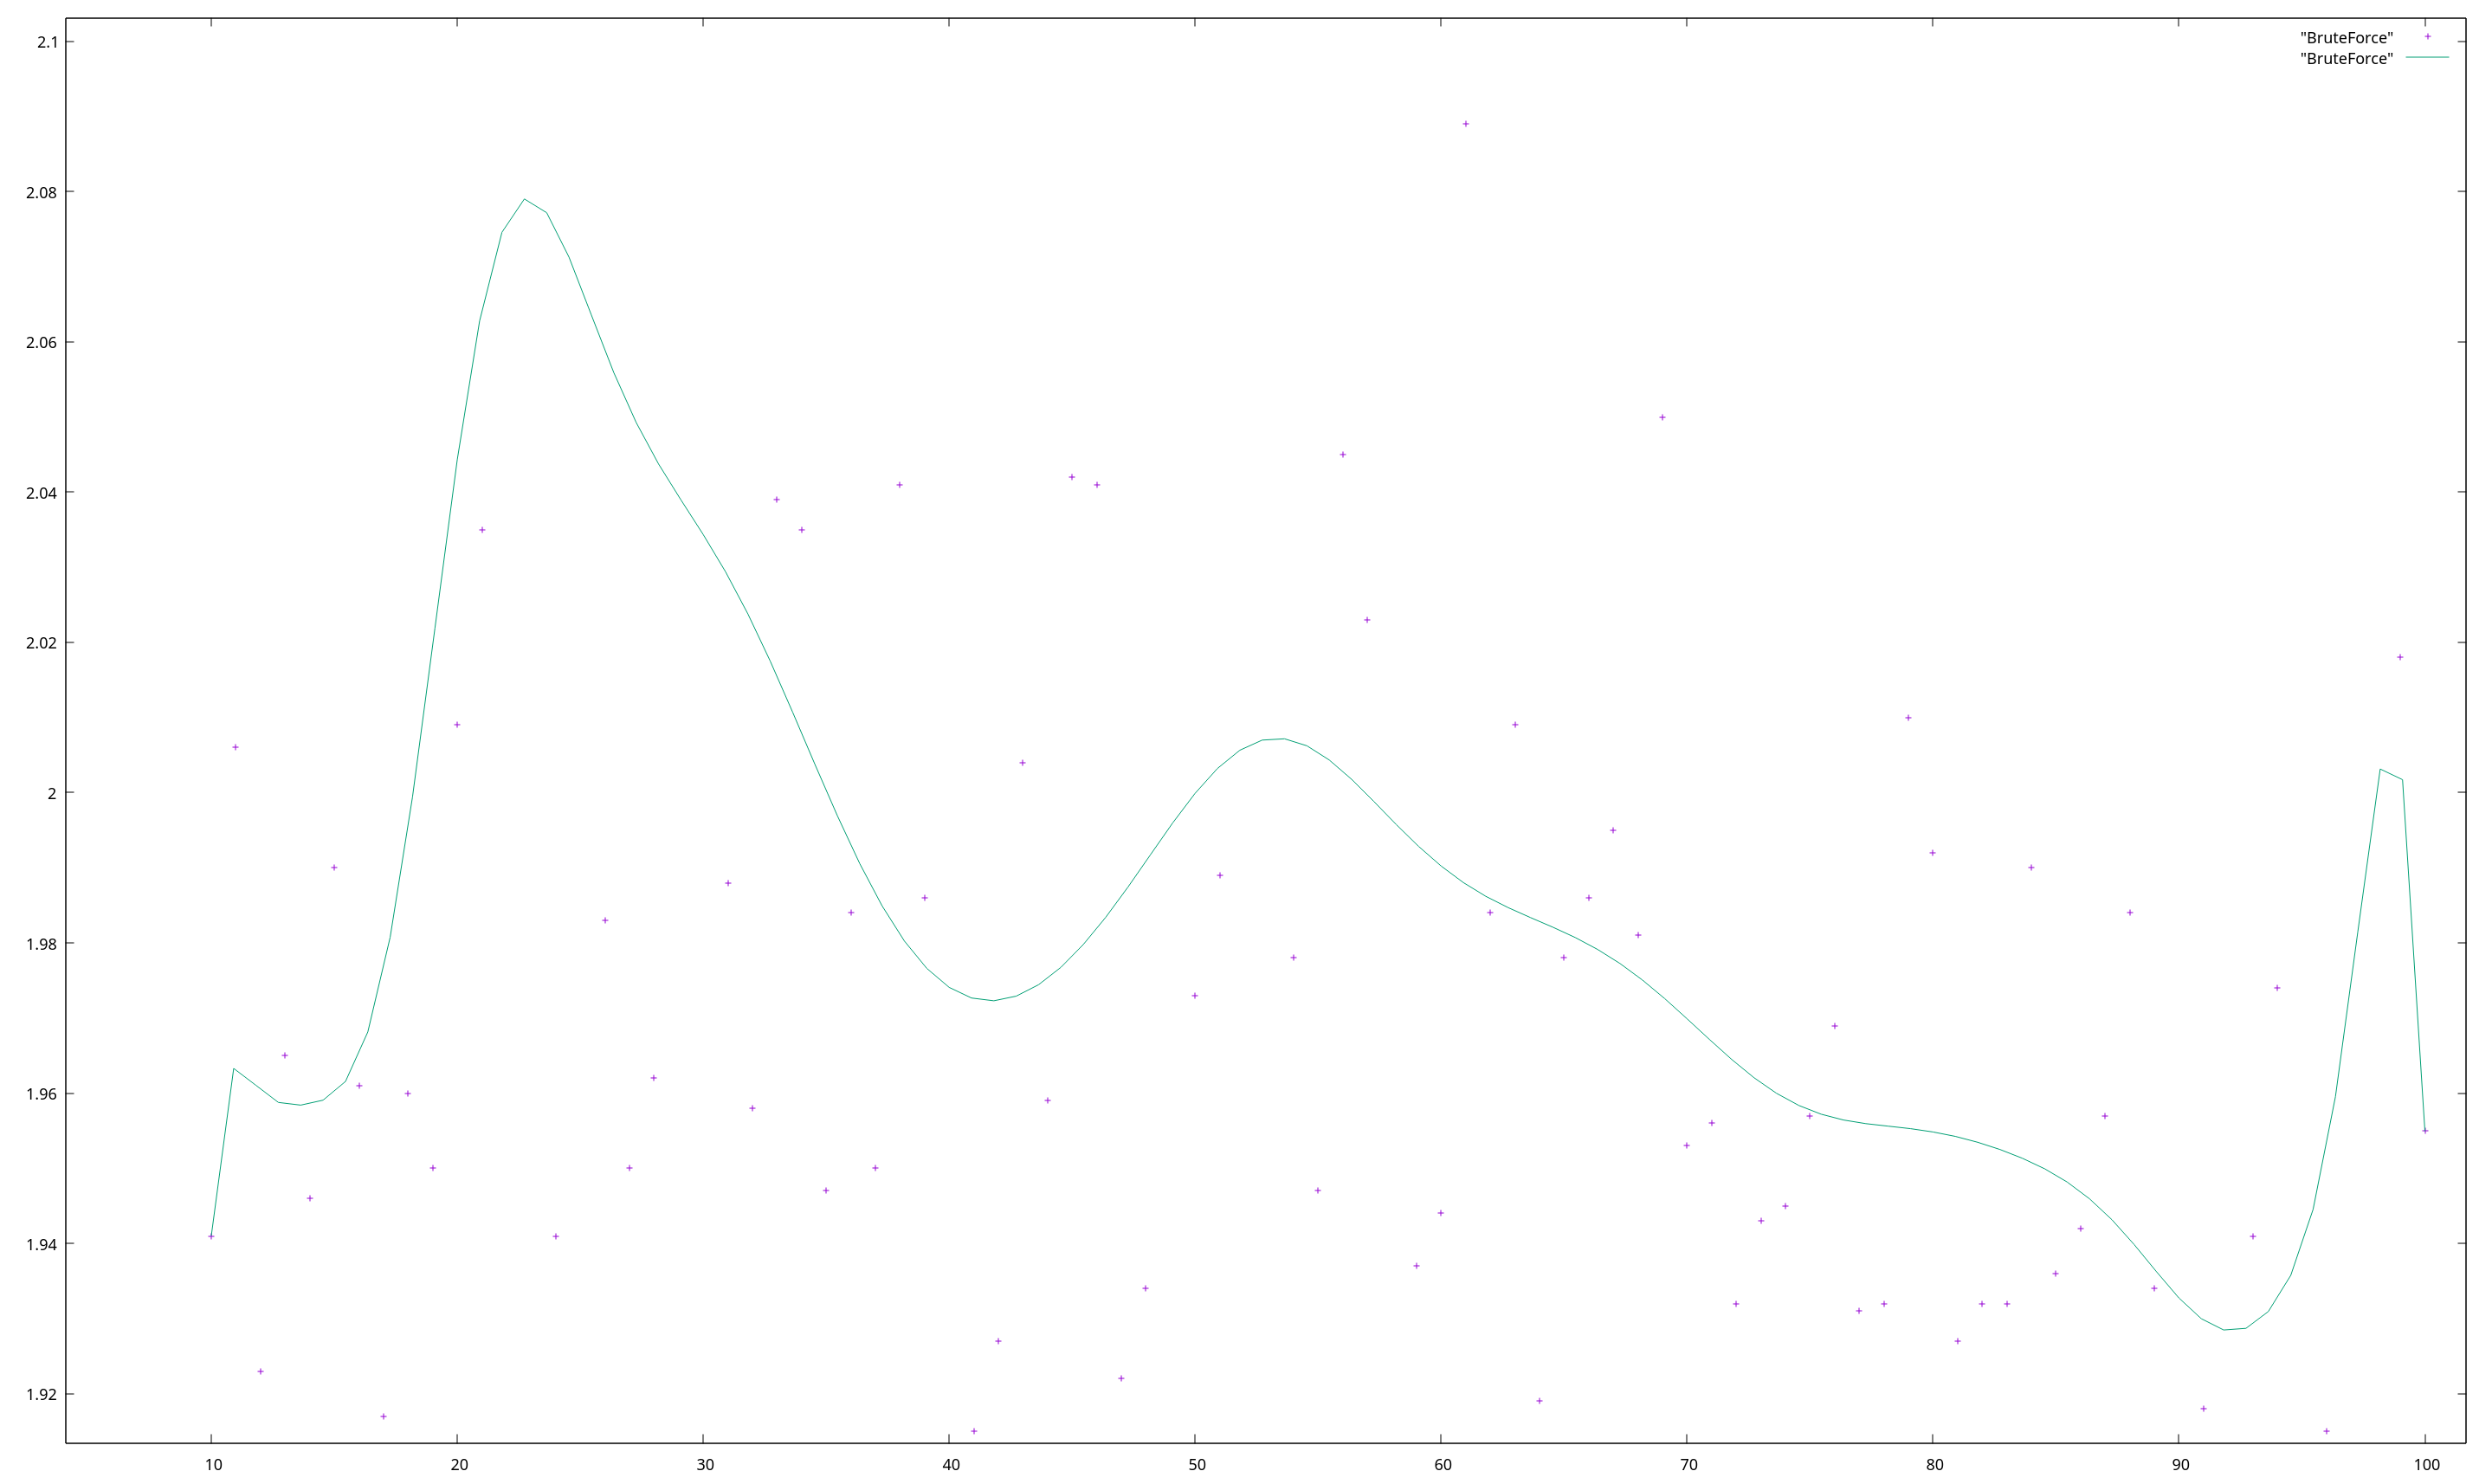
\includegraphics[width=\textwidth]{maxWeight/BruteForce}
\caption{Vývoj času výpočtu hrubou silou (pro různou maximální váhu)}
\label{maxWeight/BruteForce}
\end{center}
\end{figure}

Graf pro řešení metodou větví a hranic je zobrazen na obrázku \ref{maxWeight/BranchNBound}. Časy jsou zde mnohem kratší, okolo 0.5 milisekund. Nicméně jejich rozložení je opět lineární.

\begin{figure}[H]
\begin{center}
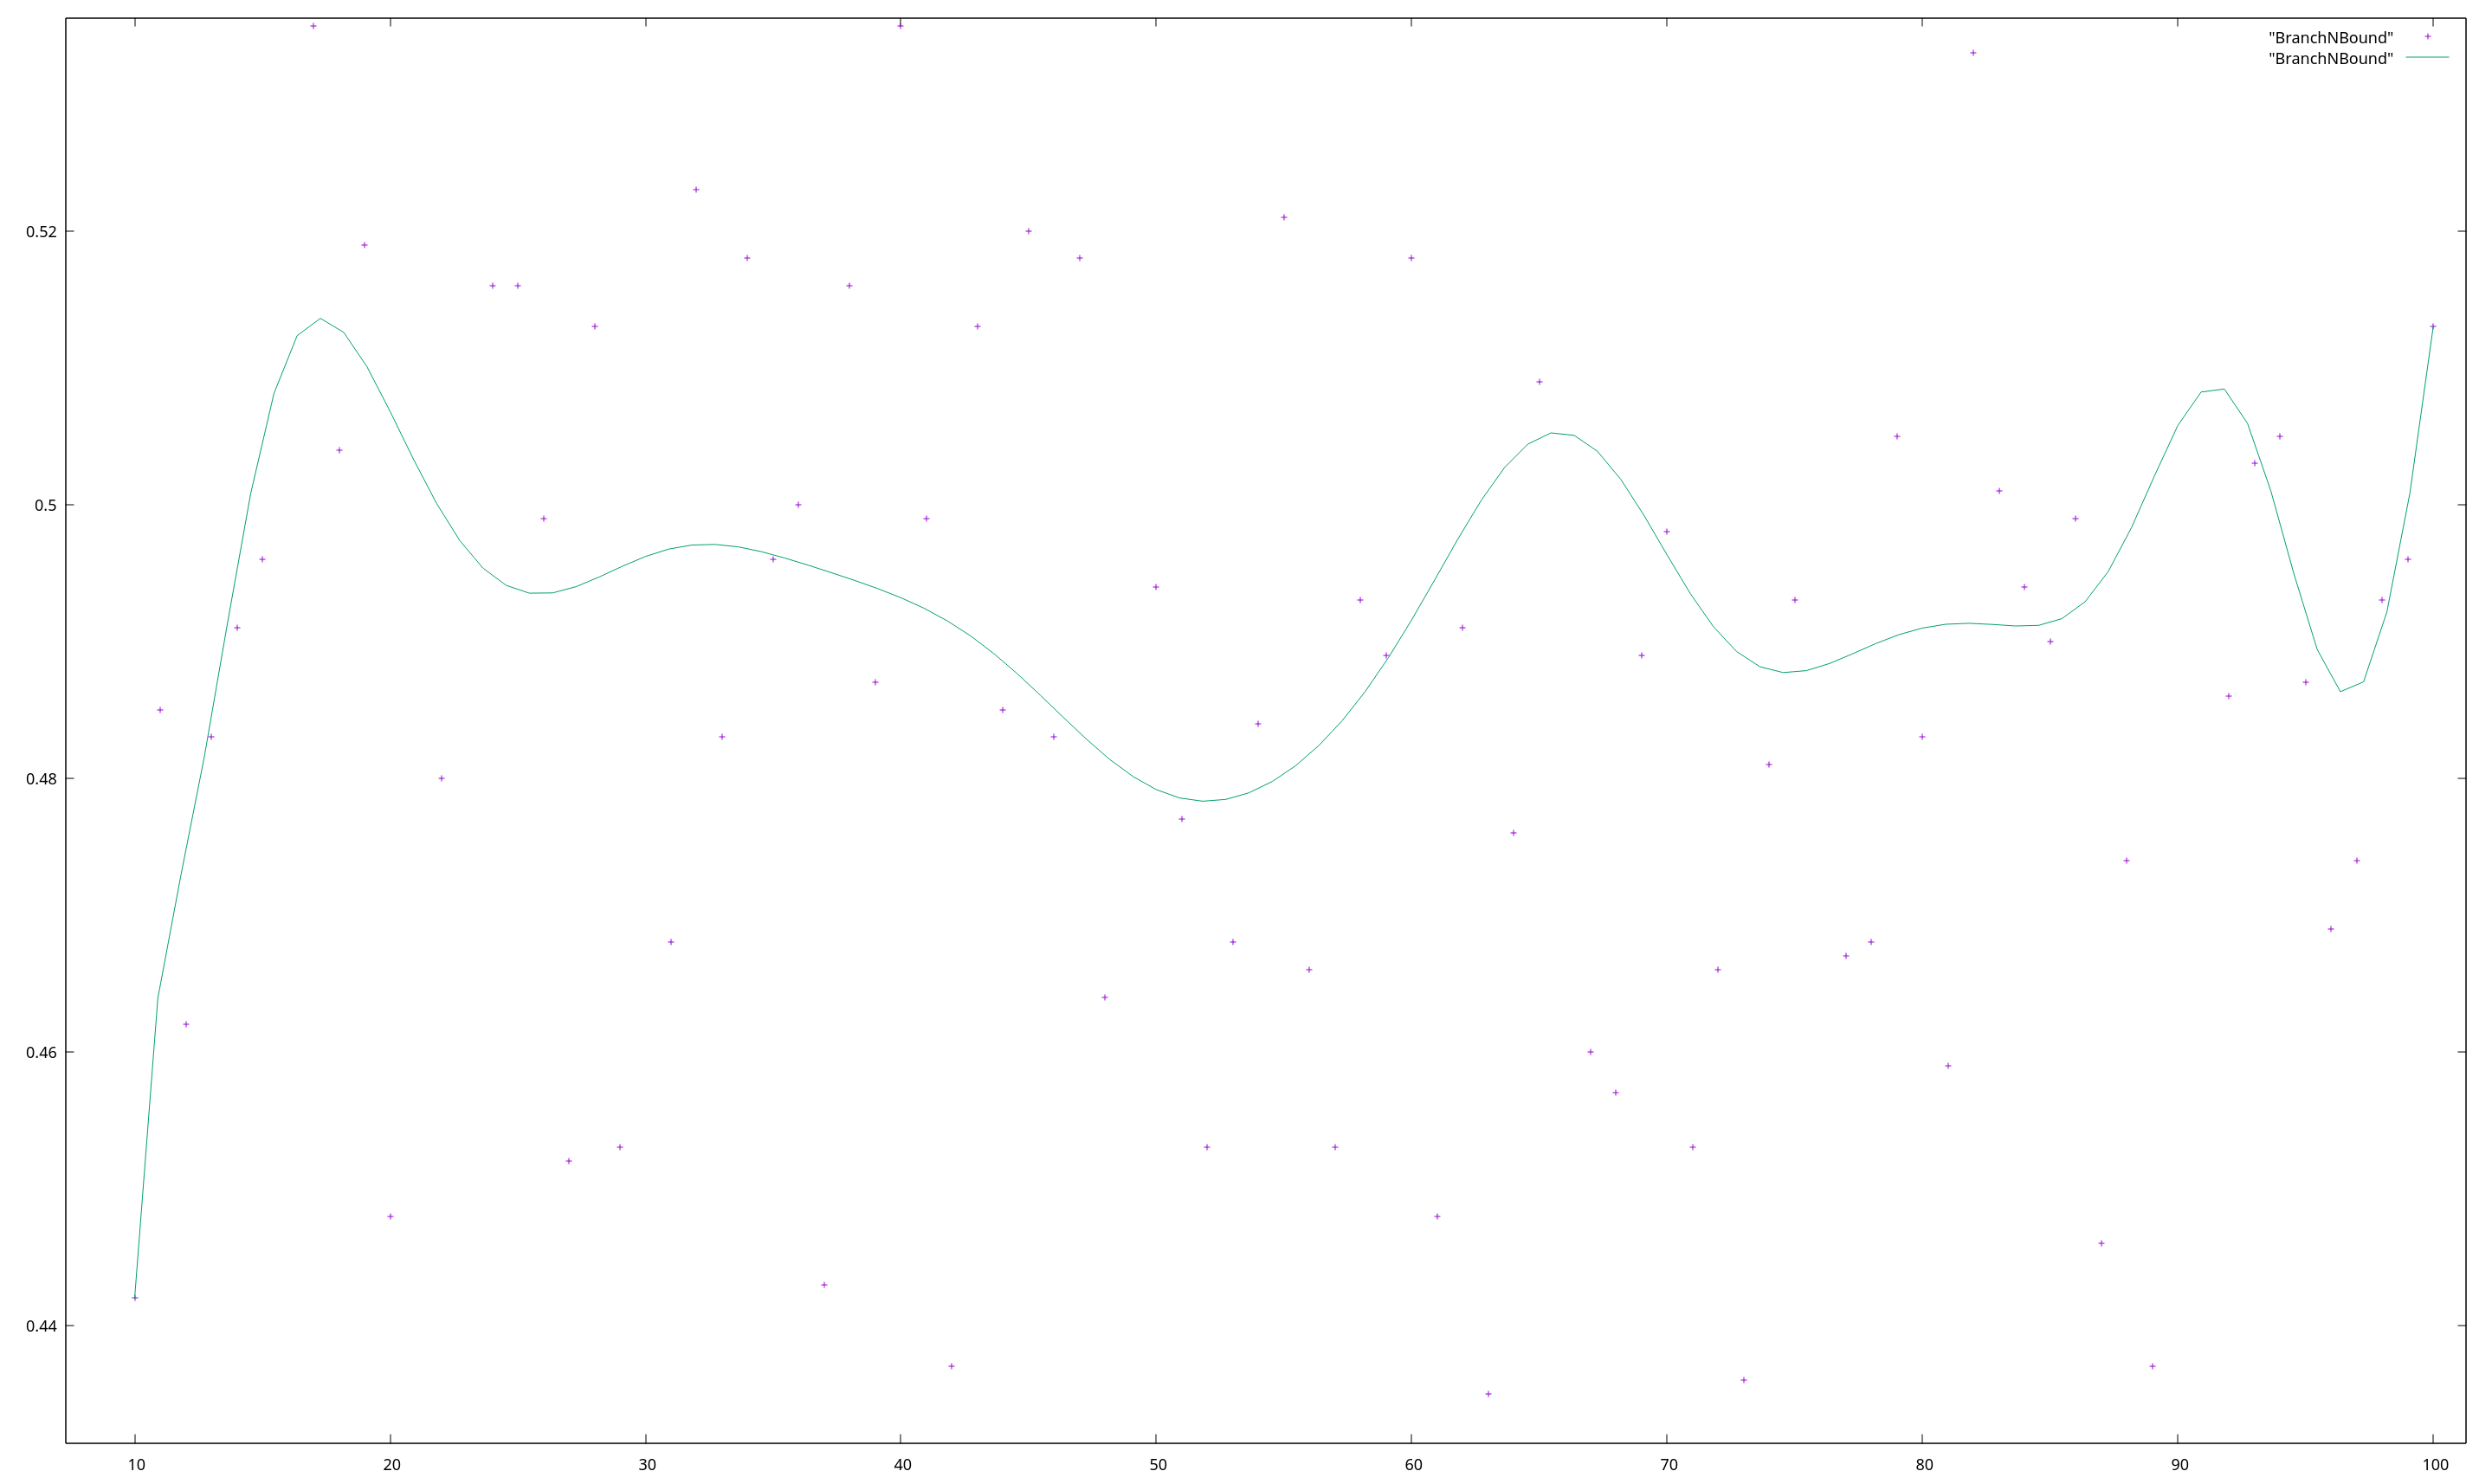
\includegraphics[width=\textwidth]{maxWeight/BranchNBound}
\caption{Vývoj času výpočtu metodou větví a hranic (pro různou maximální váhu)}
\label{maxWeight/BranchNBound}
\end{center}
\end{figure}

Řešení dynamickým programováním (dekompozicí podle ceny) je na obrázku \ref{maxWeight/PriceDecomposition}. Zde se řešní pohybuje okolo 3.9 milisekund, opět v zásadě lineárně.

\begin{figure}[H]
\begin{center}
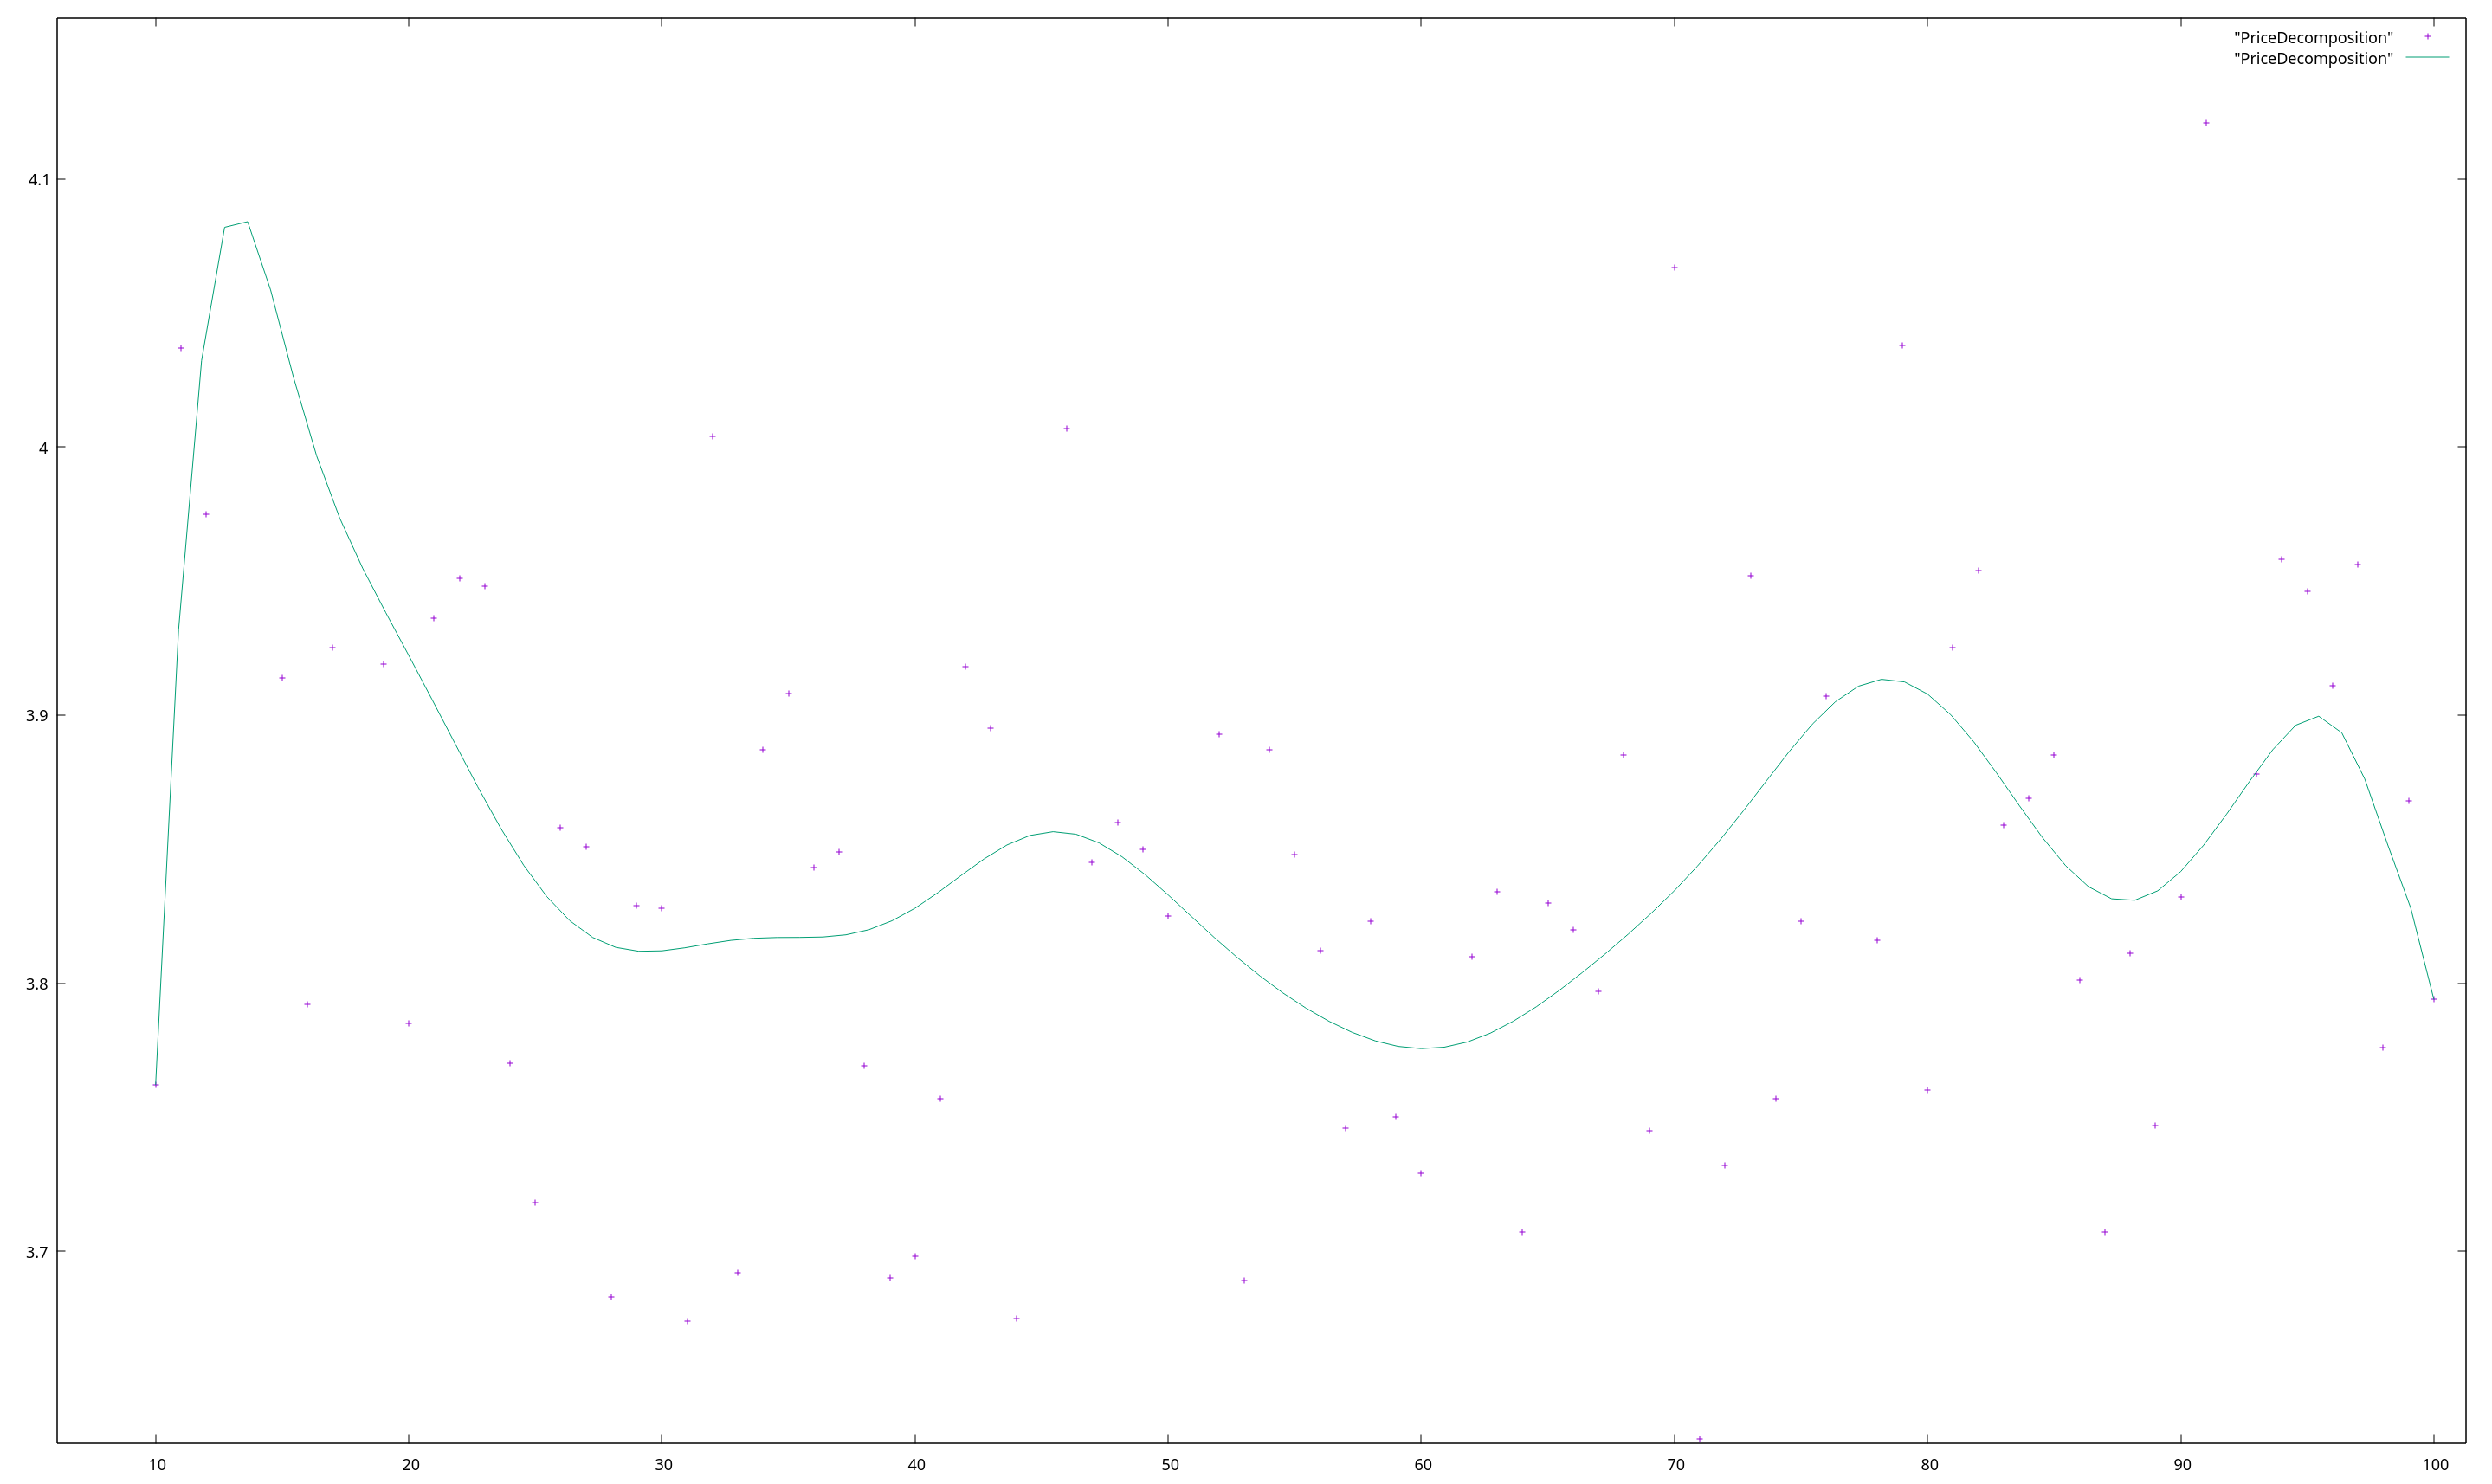
\includegraphics[width=\textwidth]{maxWeight/PriceDecomposition}
\caption{Vývoj času výpočtu dekompozicí podle ceny (pro různou maximální váhu)}
\label{maxWeight/PriceDecomposition}
\end{center}
\end{figure}

Heuristika podle poměru cena/váha je na obrázku \ref{maxWeight/PriceToWeightRatio}. Doba výpočtu se pohybuje kolem 0.142 milisekund. Rozložení je lineární.

\begin{figure}[H]
\begin{center}
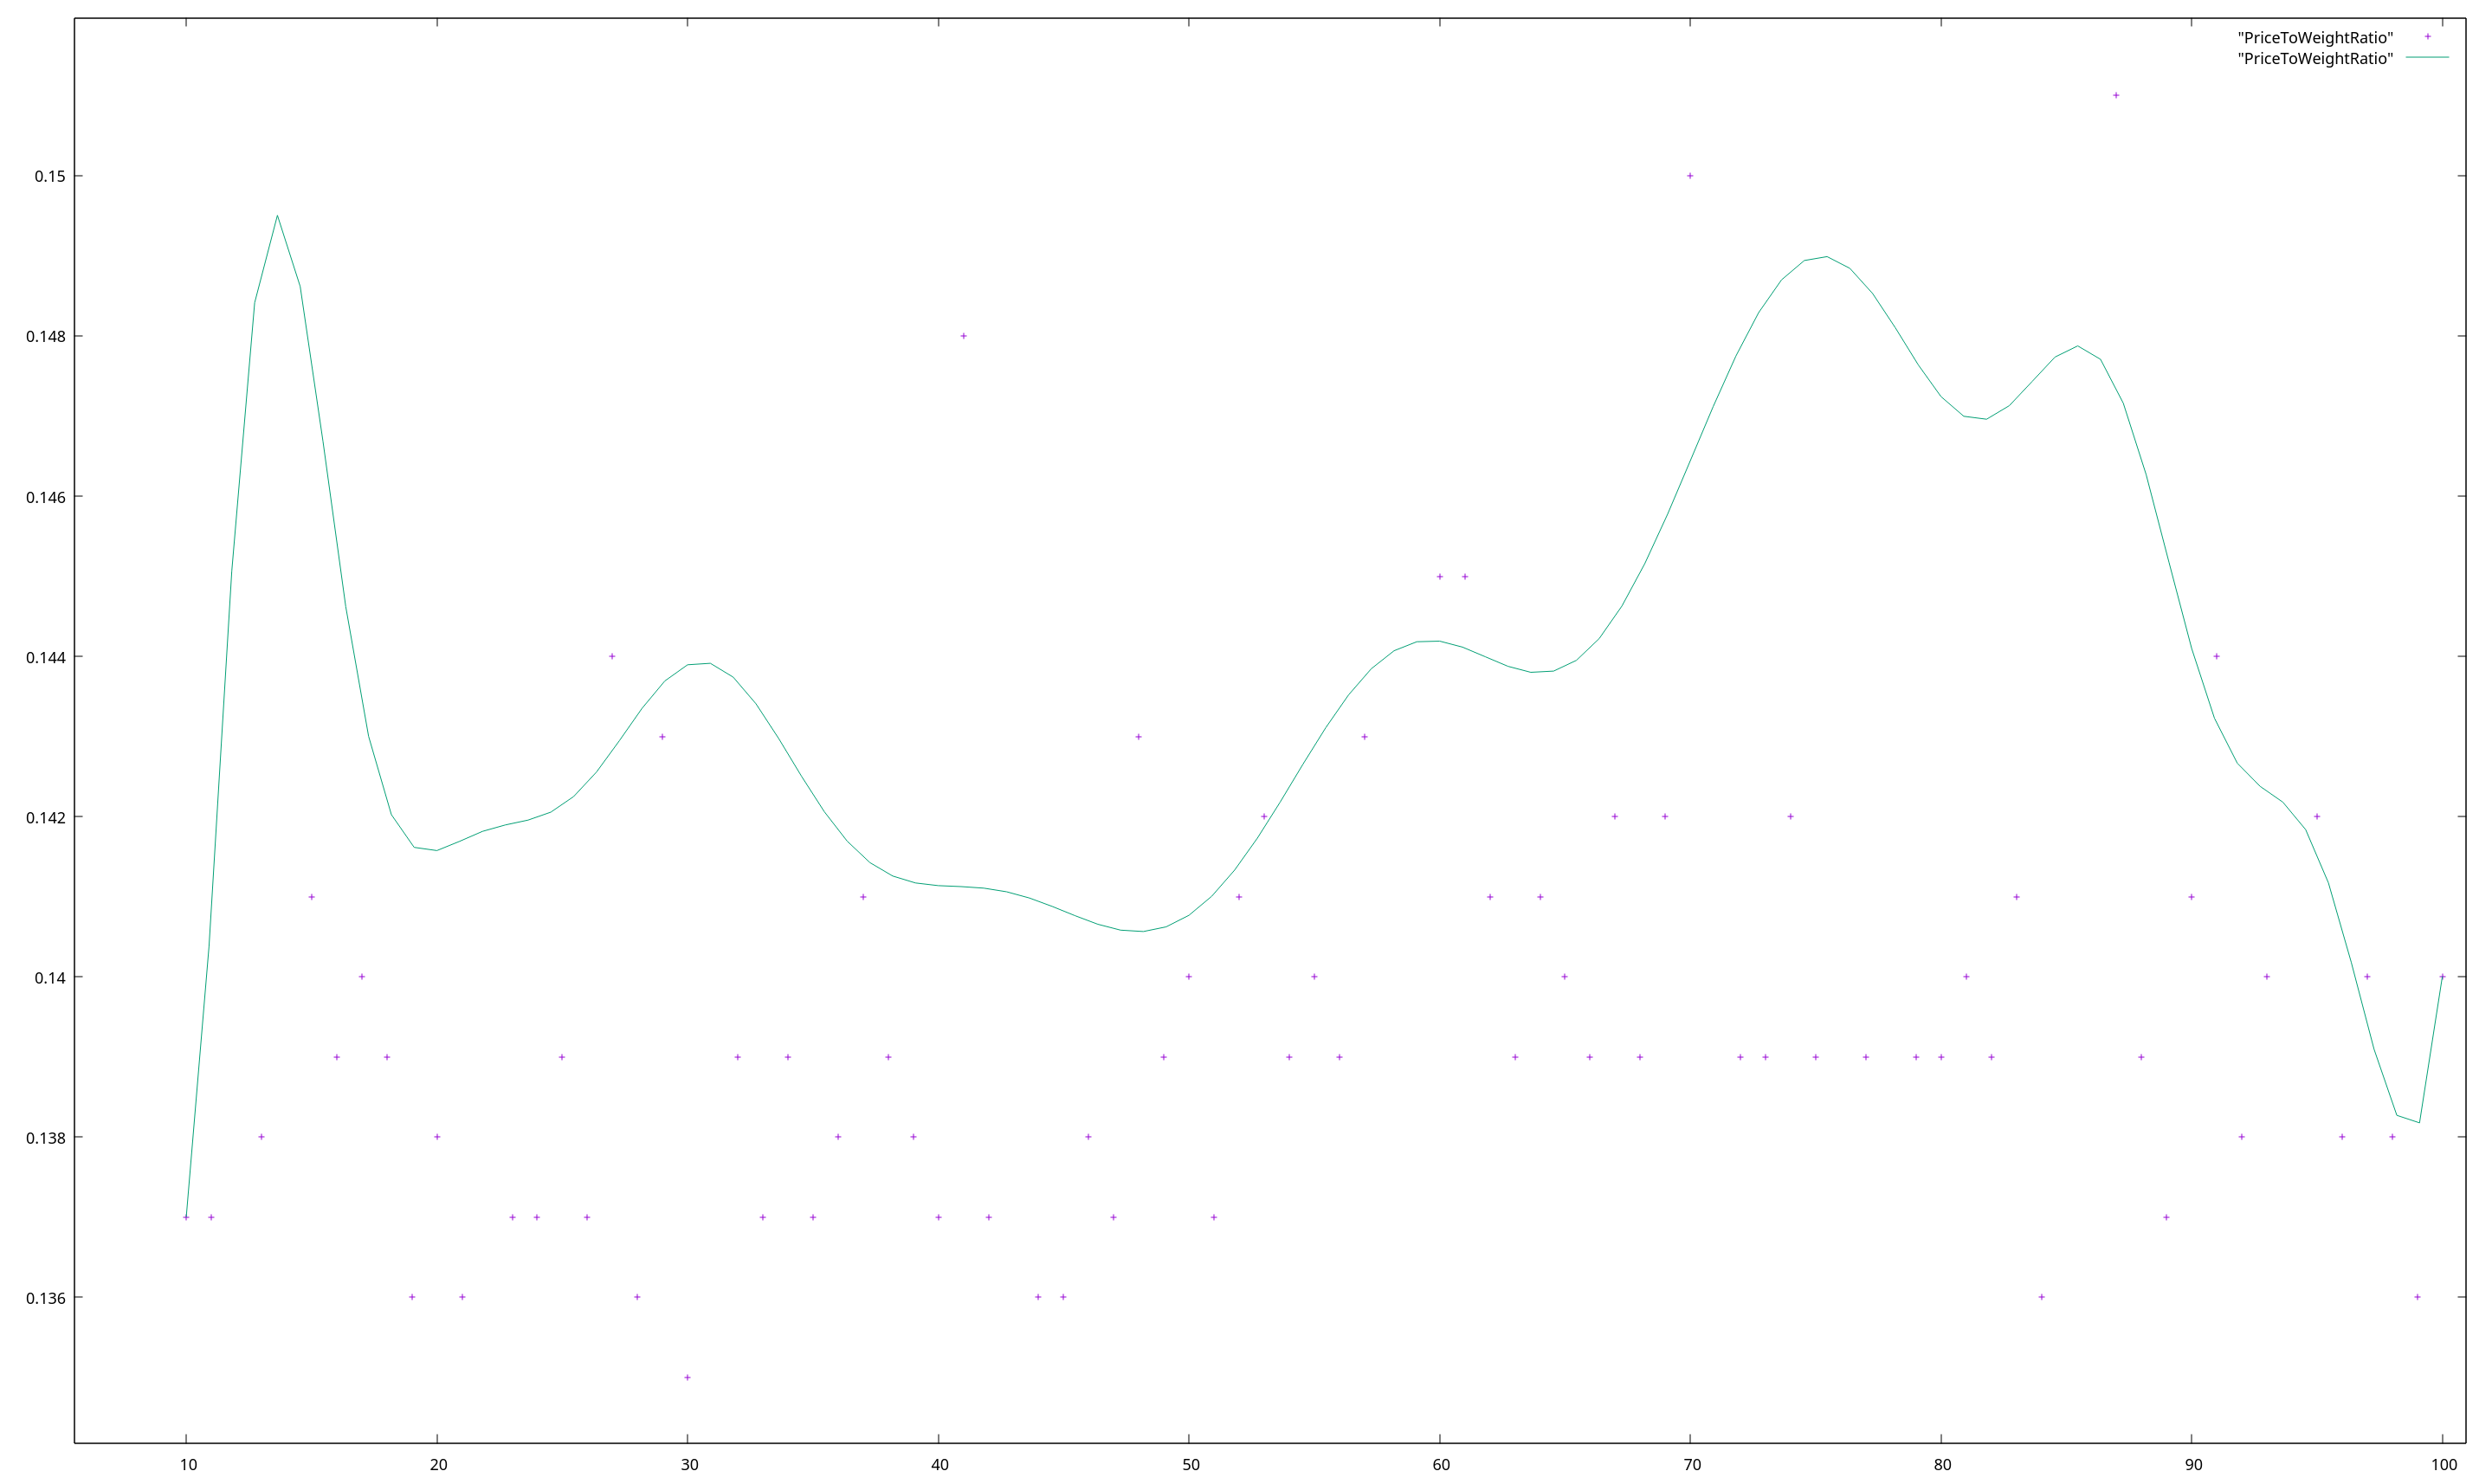
\includegraphics[width=\textwidth]{maxWeight/PriceToWeightRatio}
\caption{Vývoj času výpočtu heuristikou (pro různou maximální váhu)}
\label{maxWeight/PriceToWeightRatio}
\end{center}
\end{figure}

U heuristiky lze dále pozorovat vývoj relativní chyby, protože tento algoritmus nemusí řešit úlohu optimálně. Graf relativní chyby v závislosti na maximální váha věci je na obrázku \ref{maxWeight/PriceToWeightRatio-relerrs}. Relativní chyba se pohybuje kolem 0.04 a je, zdá se, opět lineární.

\begin{figure}[H]
\begin{center}
\includegraphics[width=\textwidth]{maxWeight/PriceToWeightRatio-relerrs}
\caption{Vývoj relativní chyby výpočtu heuristikou (pro různou maximální váhu)}
\label{maxWeight/PriceToWeightRatio-relerrs}
\end{center}
\end{figure}

Srovnání těchto metod z hlediska výpočetního času, kde je navíc lépe vidět jejich nezávislost na maximální váze, je vidět na grafu \ref{maxWeight/allExecTimes}. Nejrychleji počítá úlohu heuristika, ovšem za cenu chyby. Nejpomaleji dekompozice podle ceny, jak ale uvidíme v sekci \ref{maxCost}, je to proto, že jsou zvoleny vysoké ceny.

\begin{figure}[H]
\begin{center}
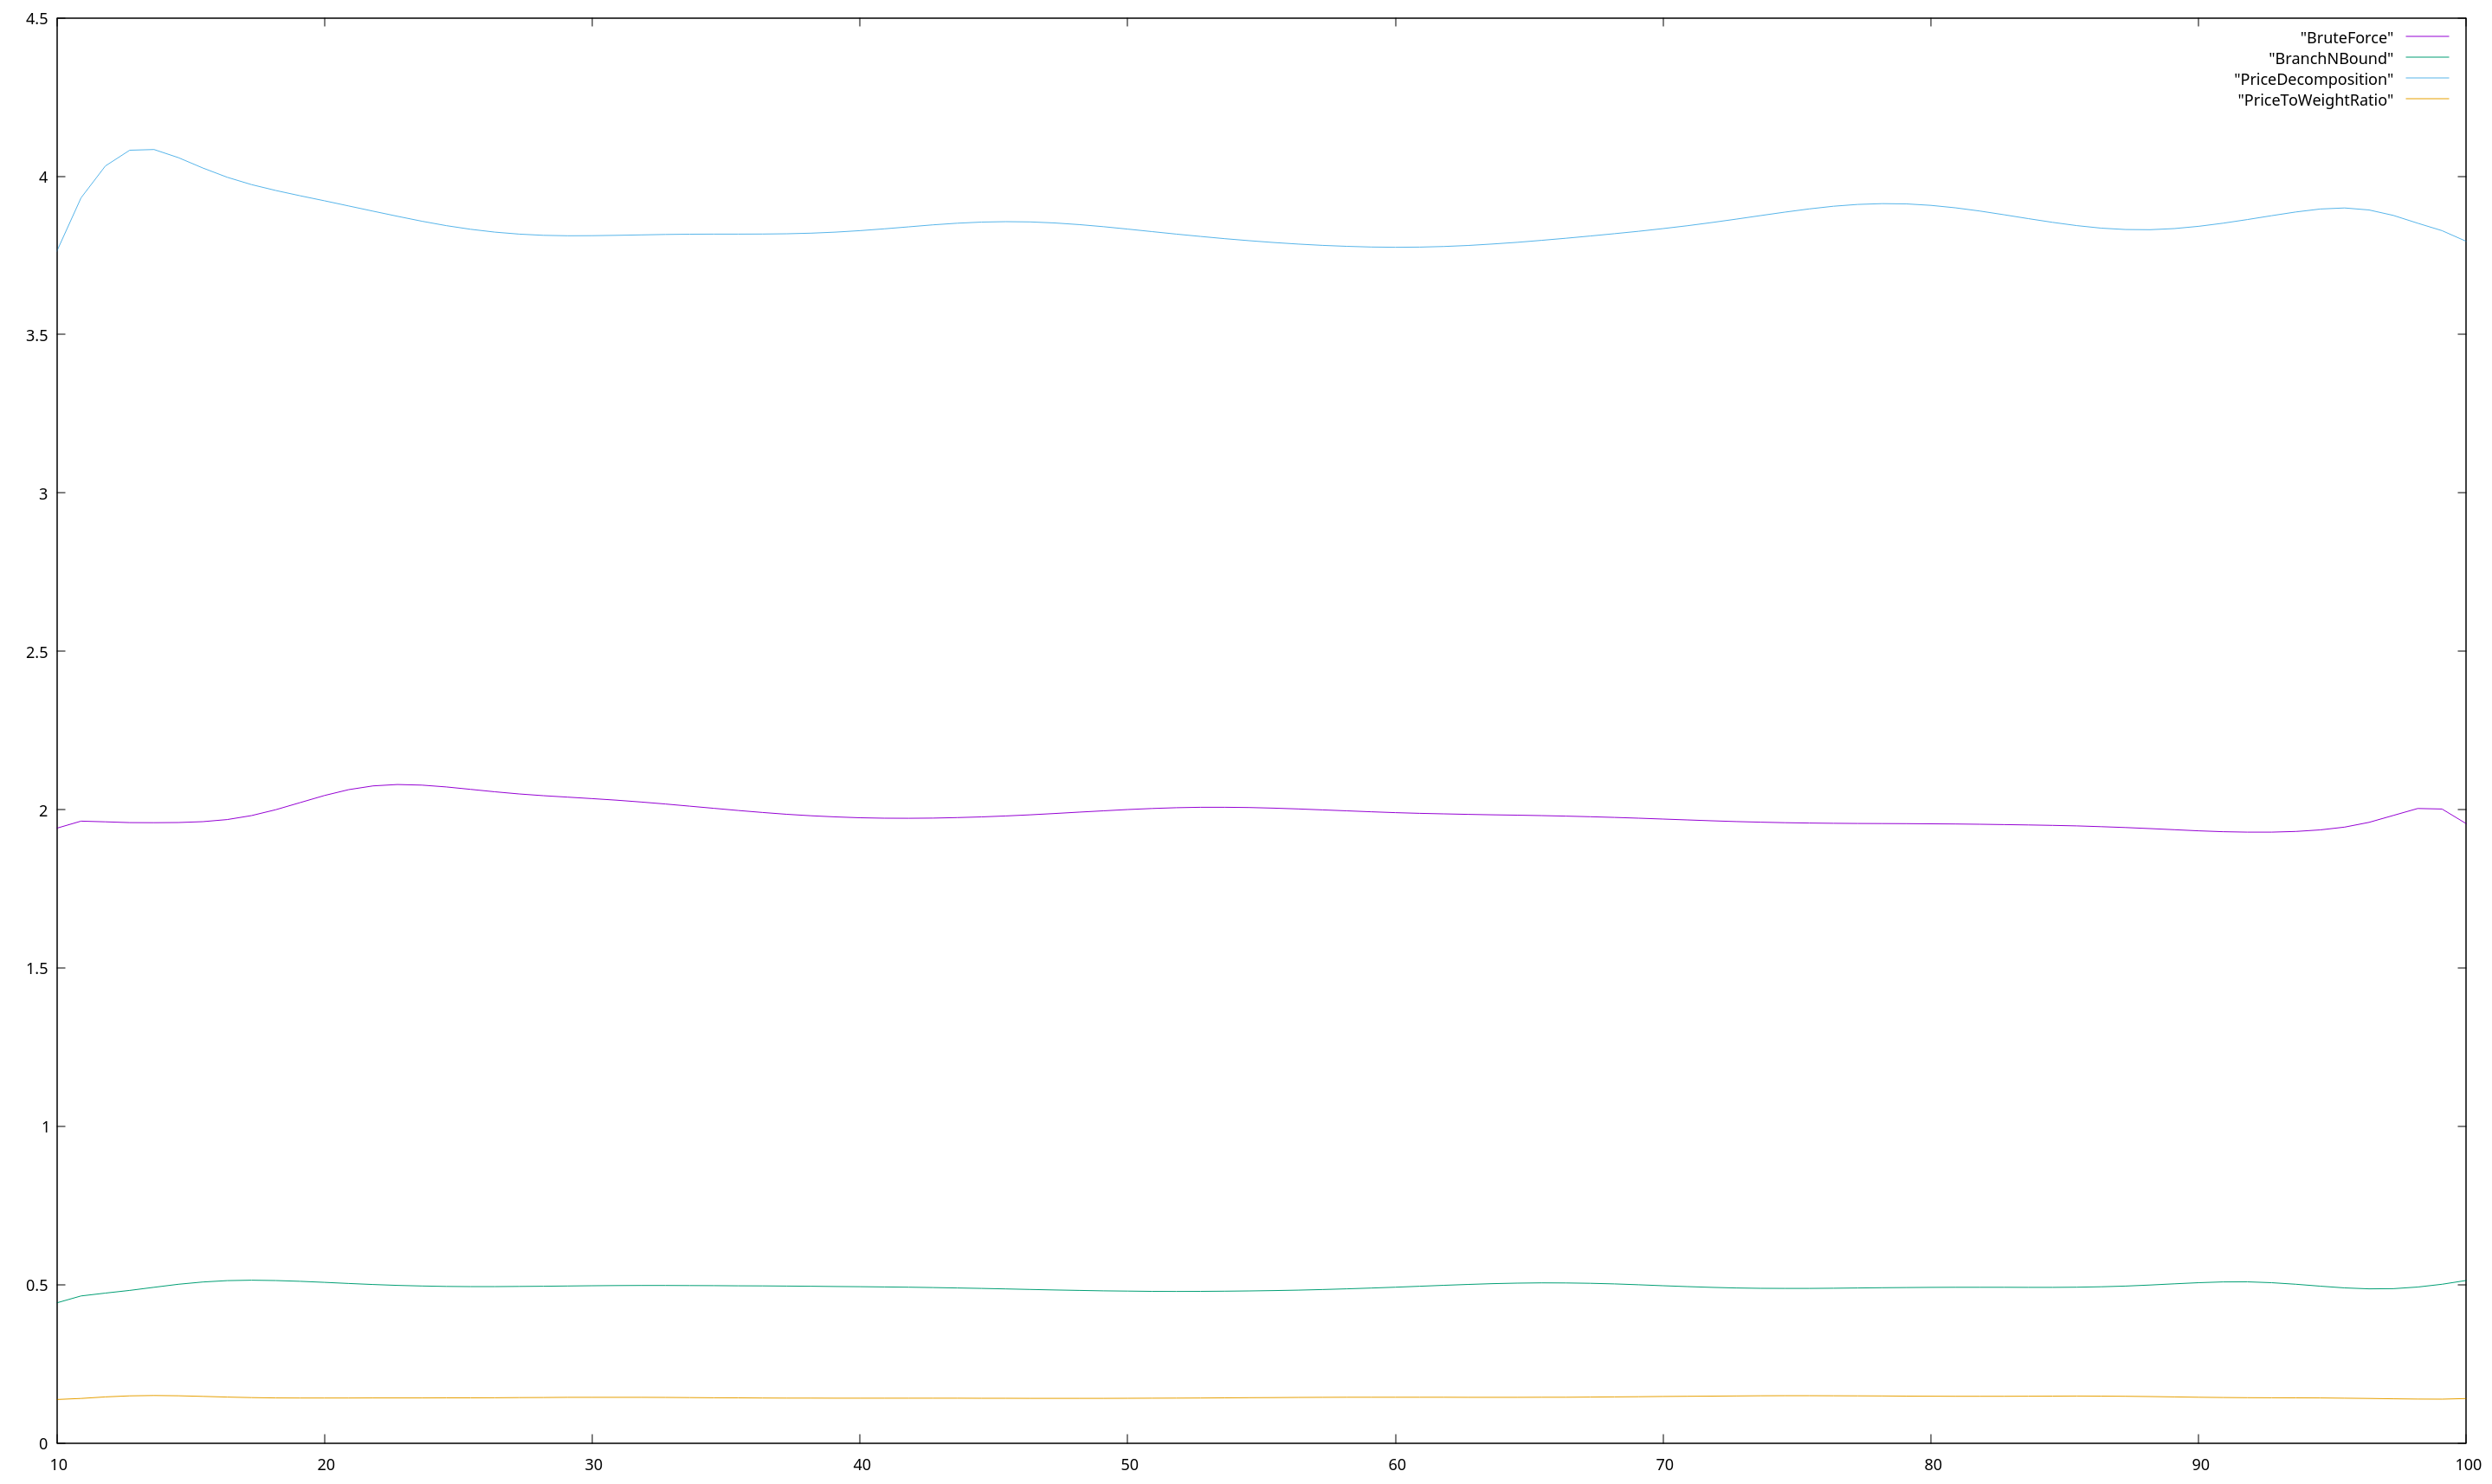
\includegraphics[width=\textwidth]{maxWeight/allExecTimes}
\caption{Srovnání závislosti metod na maximální váze}
\label{maxWeight/allExecTimes}
\end{center}
\end{figure}








\section{Změna maximální ceny}
\label{maxCost}

Dalším parametrem, který dává smysl měnit při generování instancí a pozorovat závislost jednotlivých algoritmů na něm, je maximální cena věci. Zde očekáváme, že by mohla být určitá závislost v případě dekompozice podle ceny, protože cena ovlivňuje parametr, který nezávisí na velikosti instance a který z části určuje složitost tohoto algoritmu.

Podobně jako v případě parametru maximální váhy jsem parametr maximální ceny měnil v rozsahu 10 až 100. Tím jsem opět získal 91 různých měření, každé provedené na 50 vygenerovaných instancí těchto vlastností.

Graf závislosti času výpočtu hrubou silou na parametru maximální ceny je na obrázku \ref{maxCost/BruteForce}. Čas výpočtu se pohybuje stejně jako v sekci \ref{maxWeight} okolo 2 milisekund a je náhodný.

\begin{figure}[H]
\begin{center}
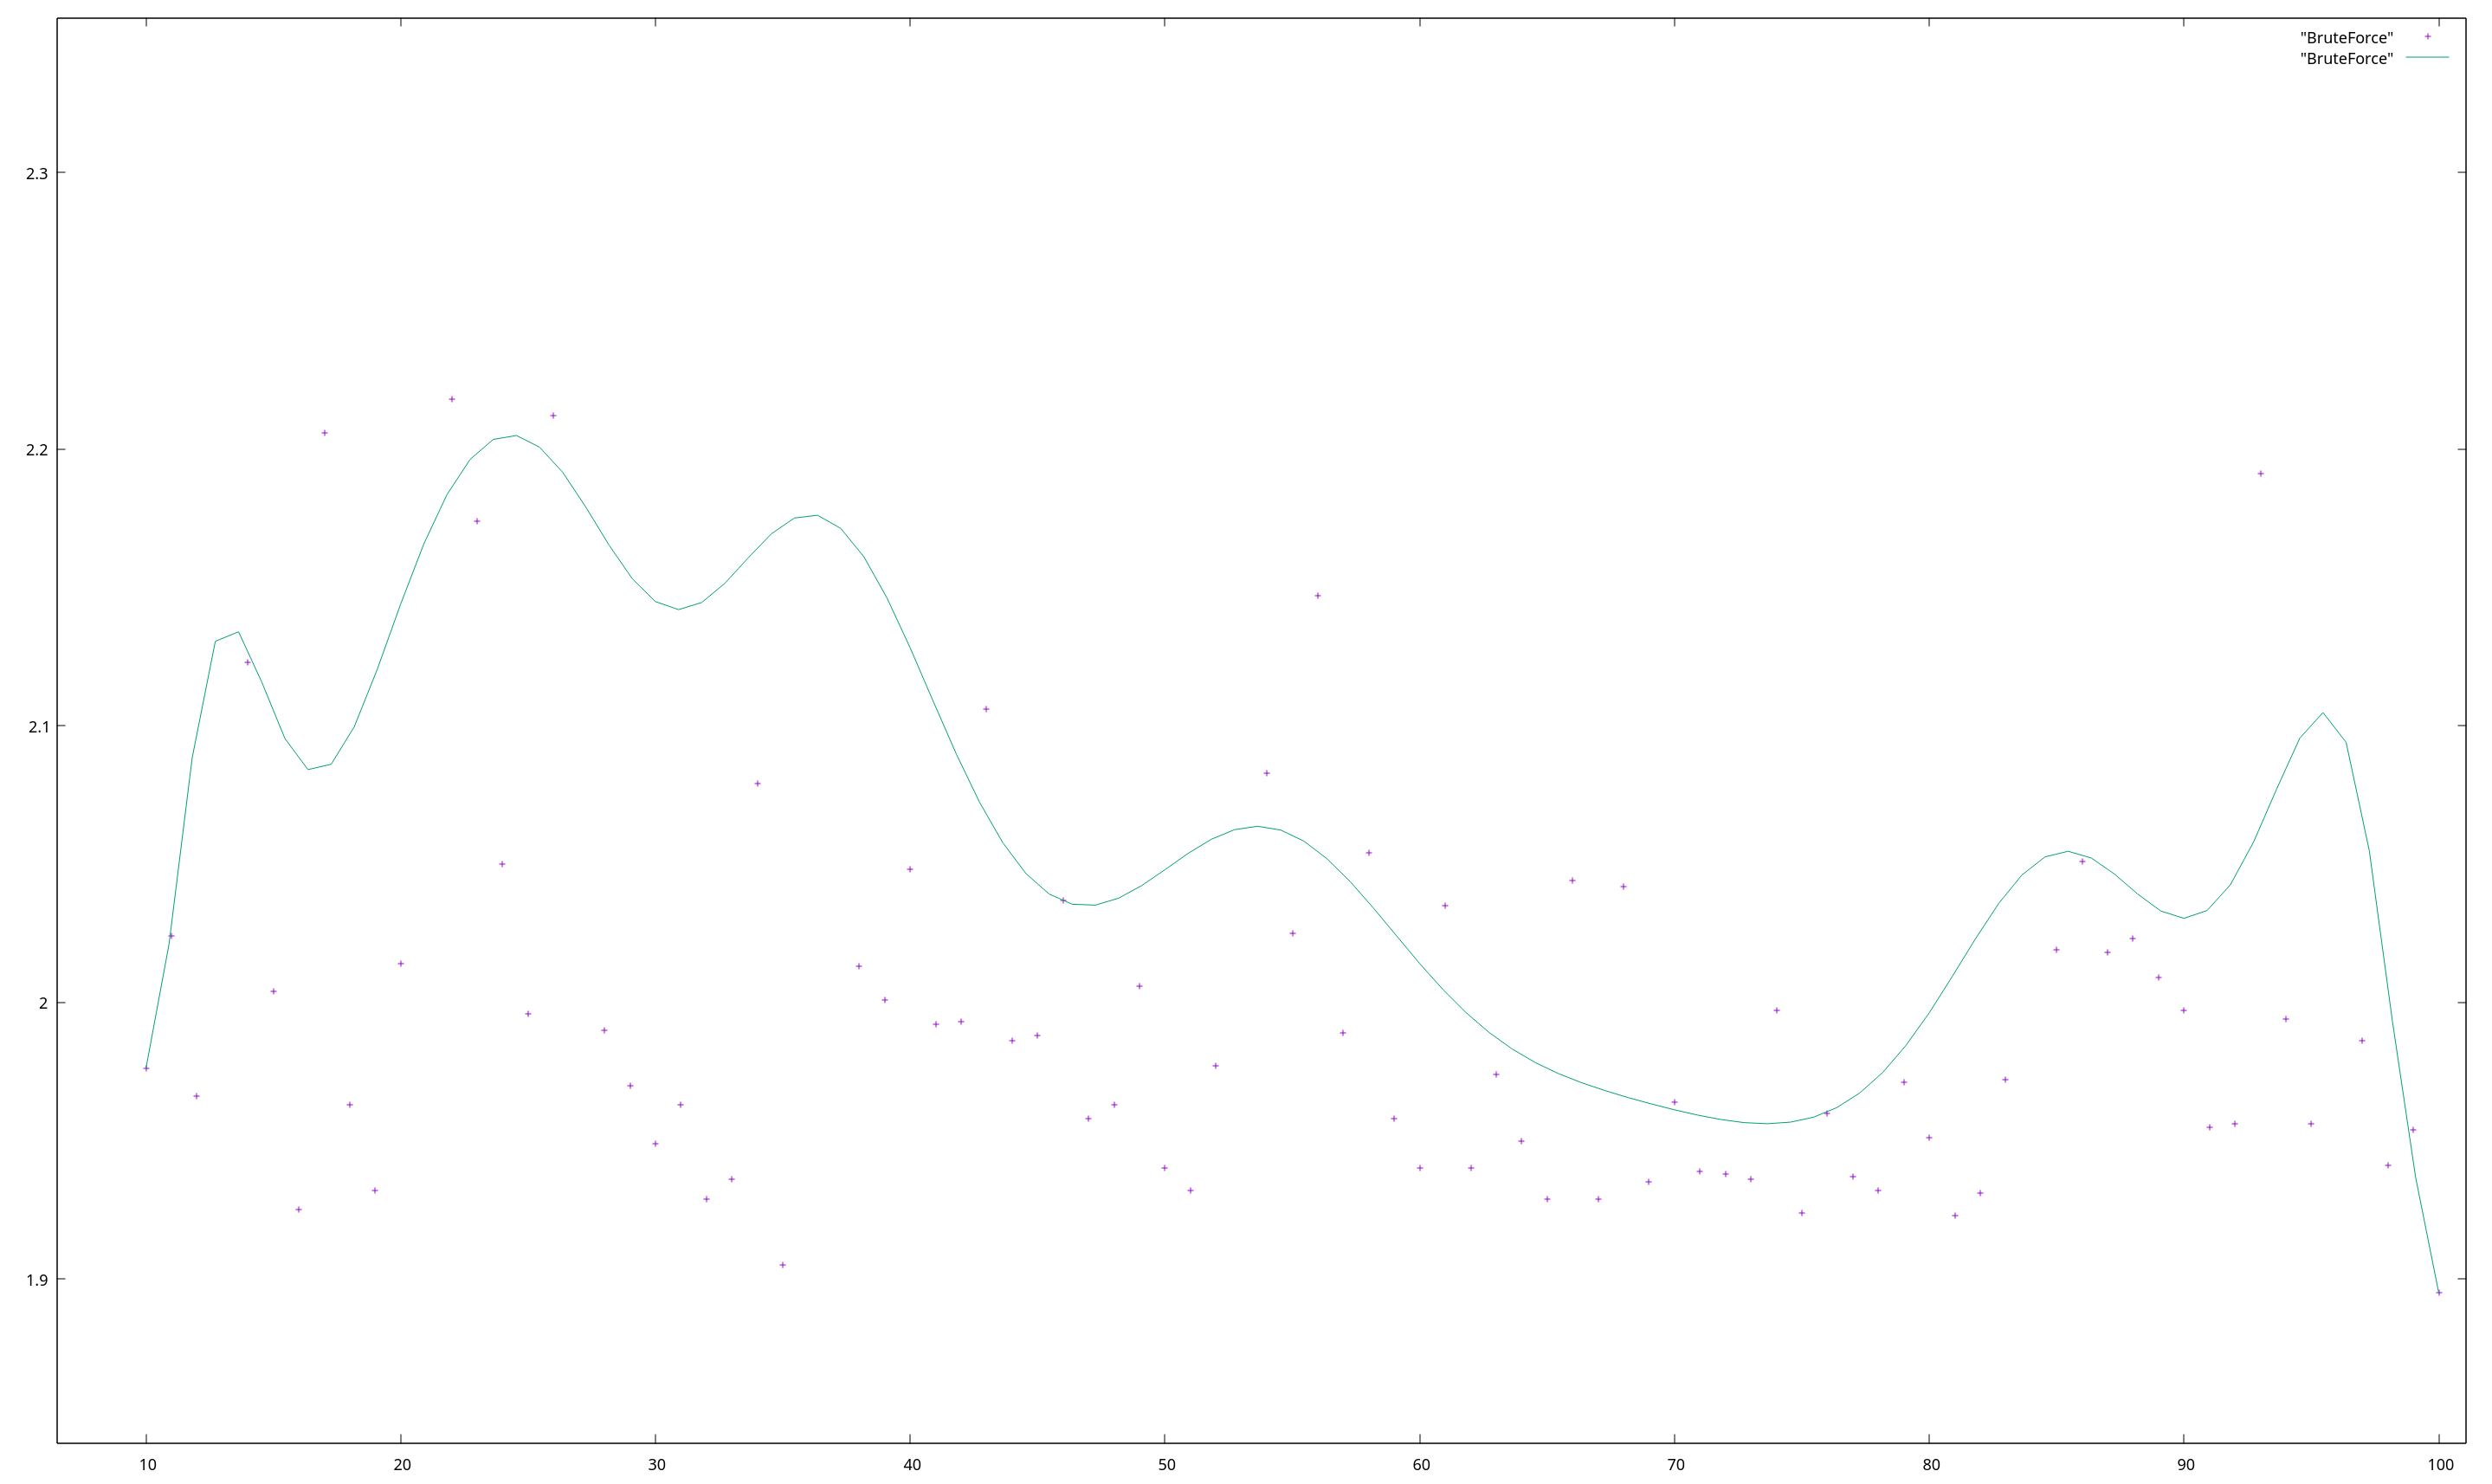
\includegraphics[width=\textwidth]{maxCost/BruteForce}
\caption{Vývoj času výpočtu hrubou silou (pro různou maximální cenu)}
\label{maxCost/BruteForce}
\end{center}
\end{figure}

Graf závislosti času na maximální ceně pro řešení metodou větví a hranic je na obrázku \ref{maxCost/BranchNBound}. Čas výpočtu je opět jako v sekci \ref{maxWeight} okolo půl milisekundy a je opět náhodný.

\begin{figure}[H]
\begin{center}
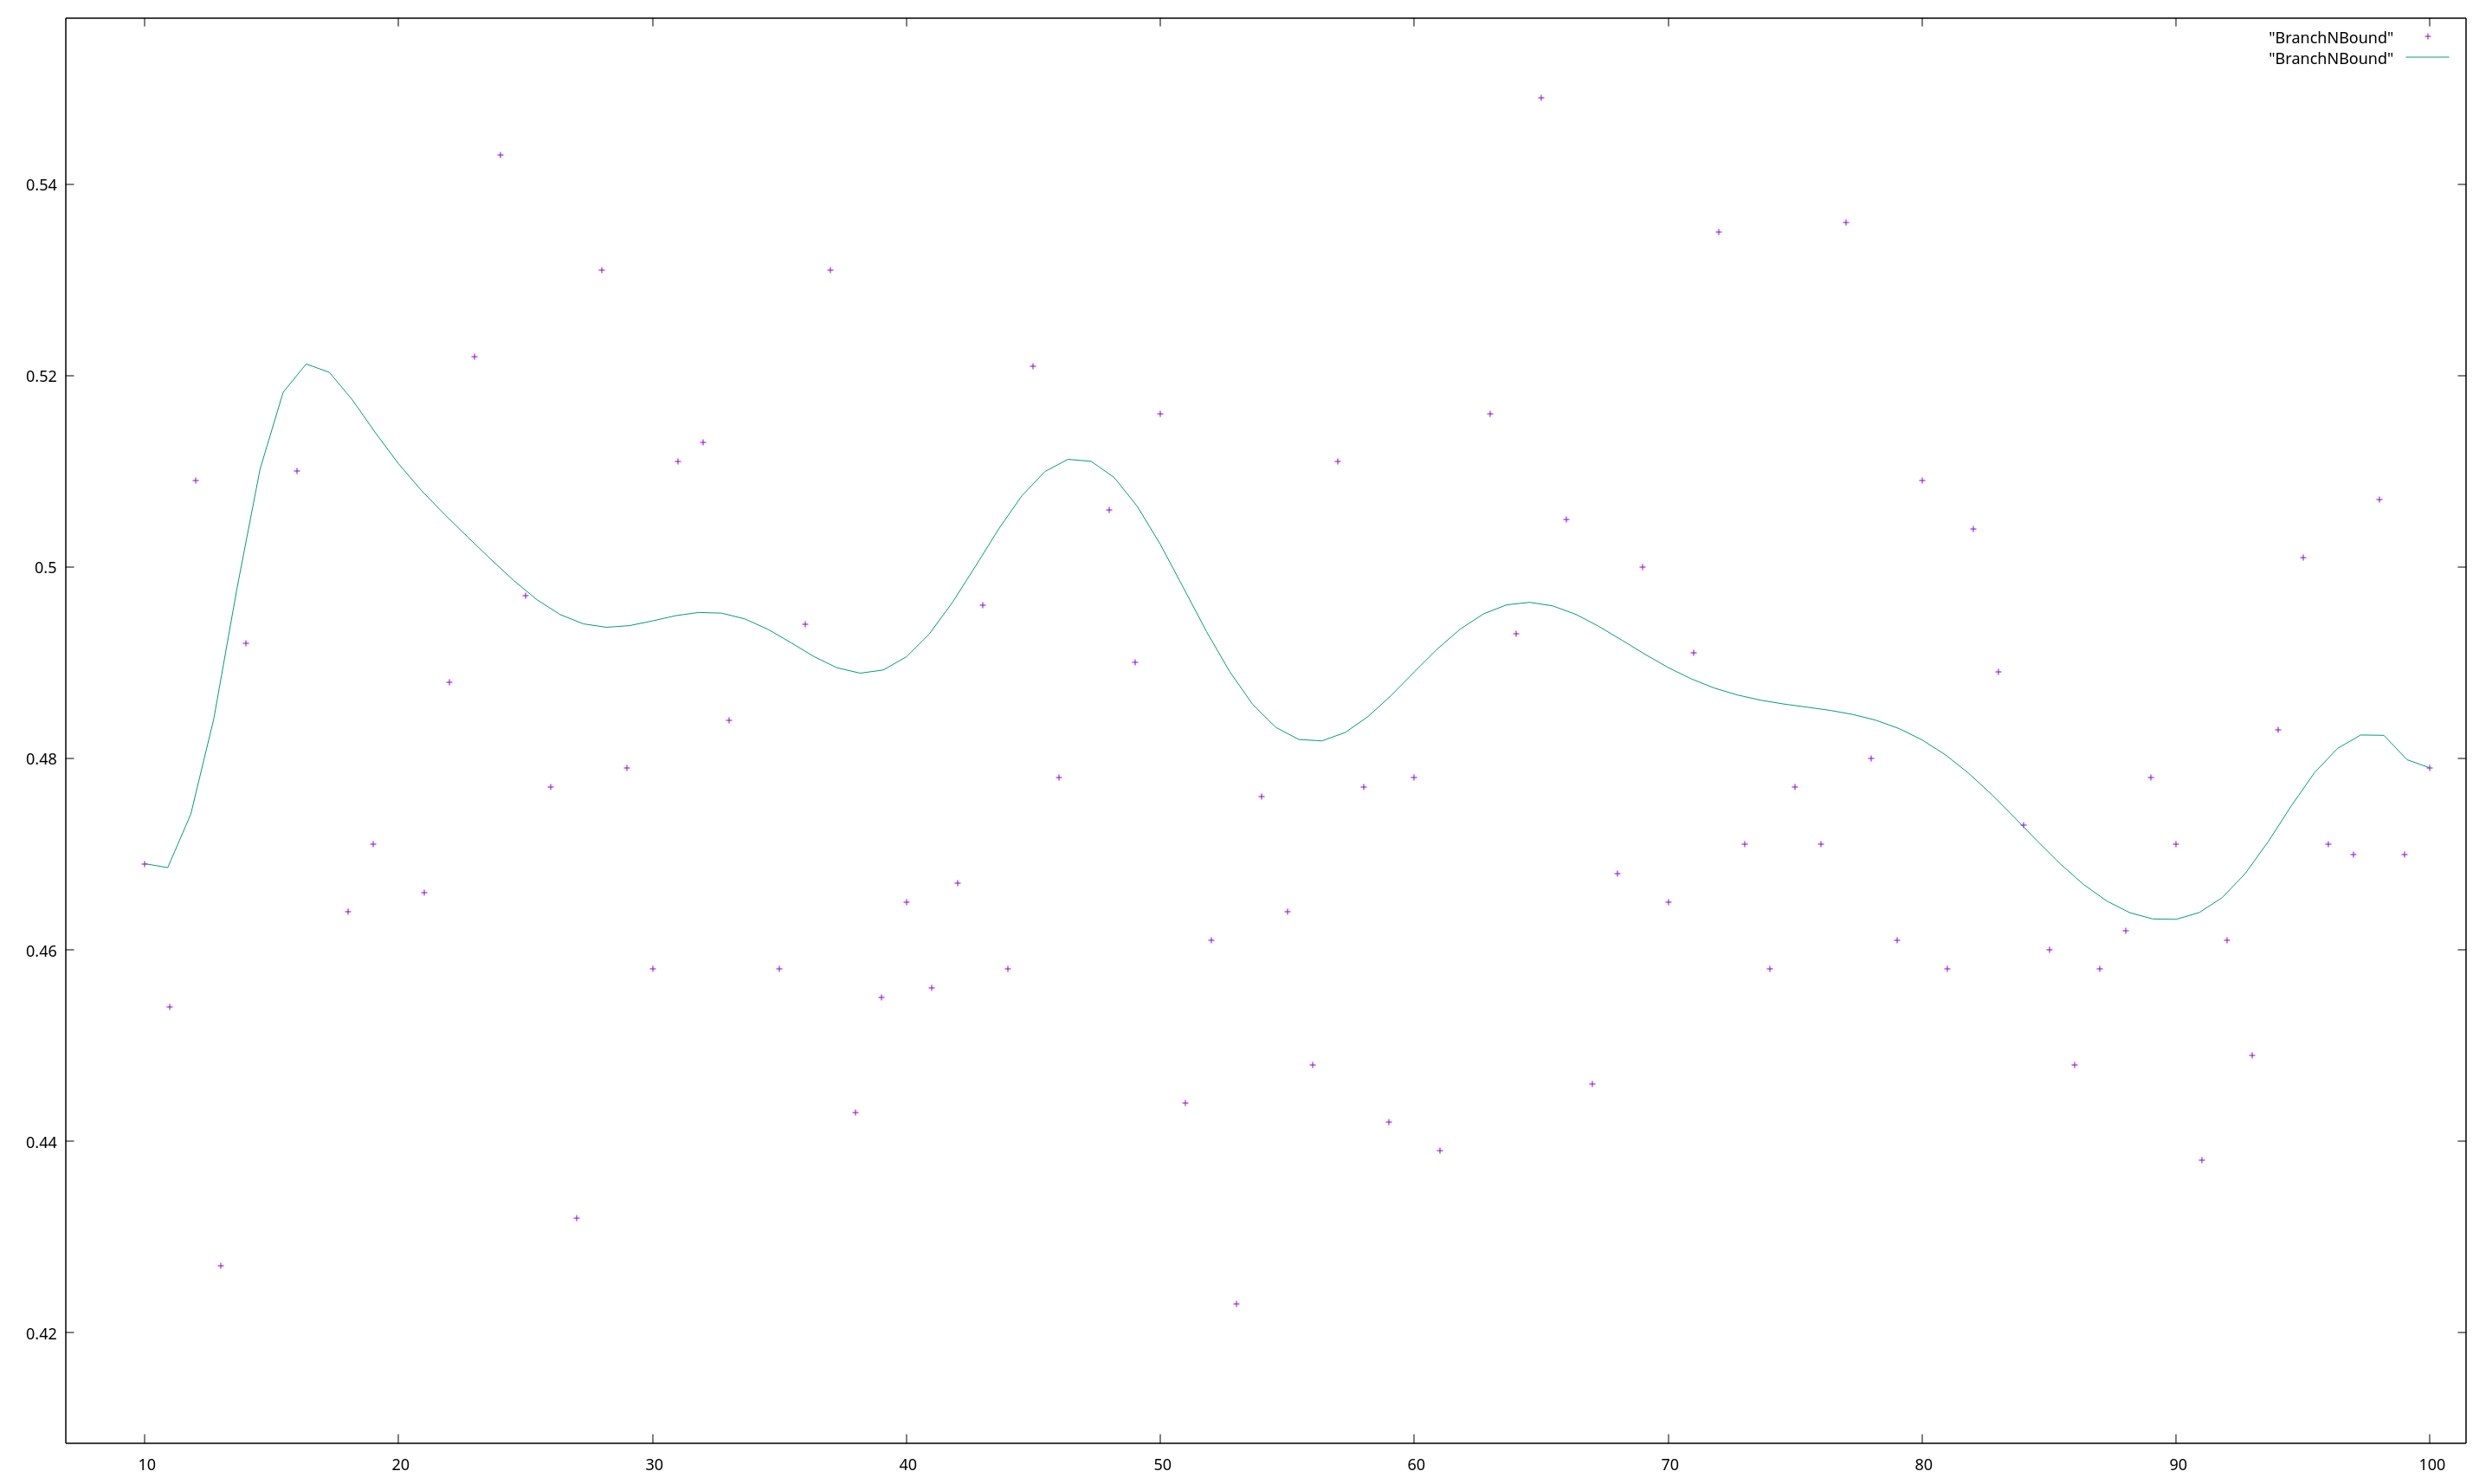
\includegraphics[width=\textwidth]{maxCost/BranchNBound}
\caption{Vývoj času výpočtu metodou větví a hranic (pro různou maximální cenu)}
\label{maxCost/BranchNBound}
\end{center}
\end{figure}

Nyní je na řadě první zajímavější graf, obrázek \ref{maxCost/PriceDecomposition}. Zobrazuje závislost času výpočtu na maximální ceně pro dekompizici podle ceny. Dle očekávání s vyšší maximální cenou čas výpočtu roste. Růst se zdá být téměř lineární. Tento výsledek odpovídá skutečnosti, že složitost tohoto algoritmu závisí lineárně na parametru ceny, který přímo nesouvisí s velikostí instance.

\begin{figure}[H]
\begin{center}
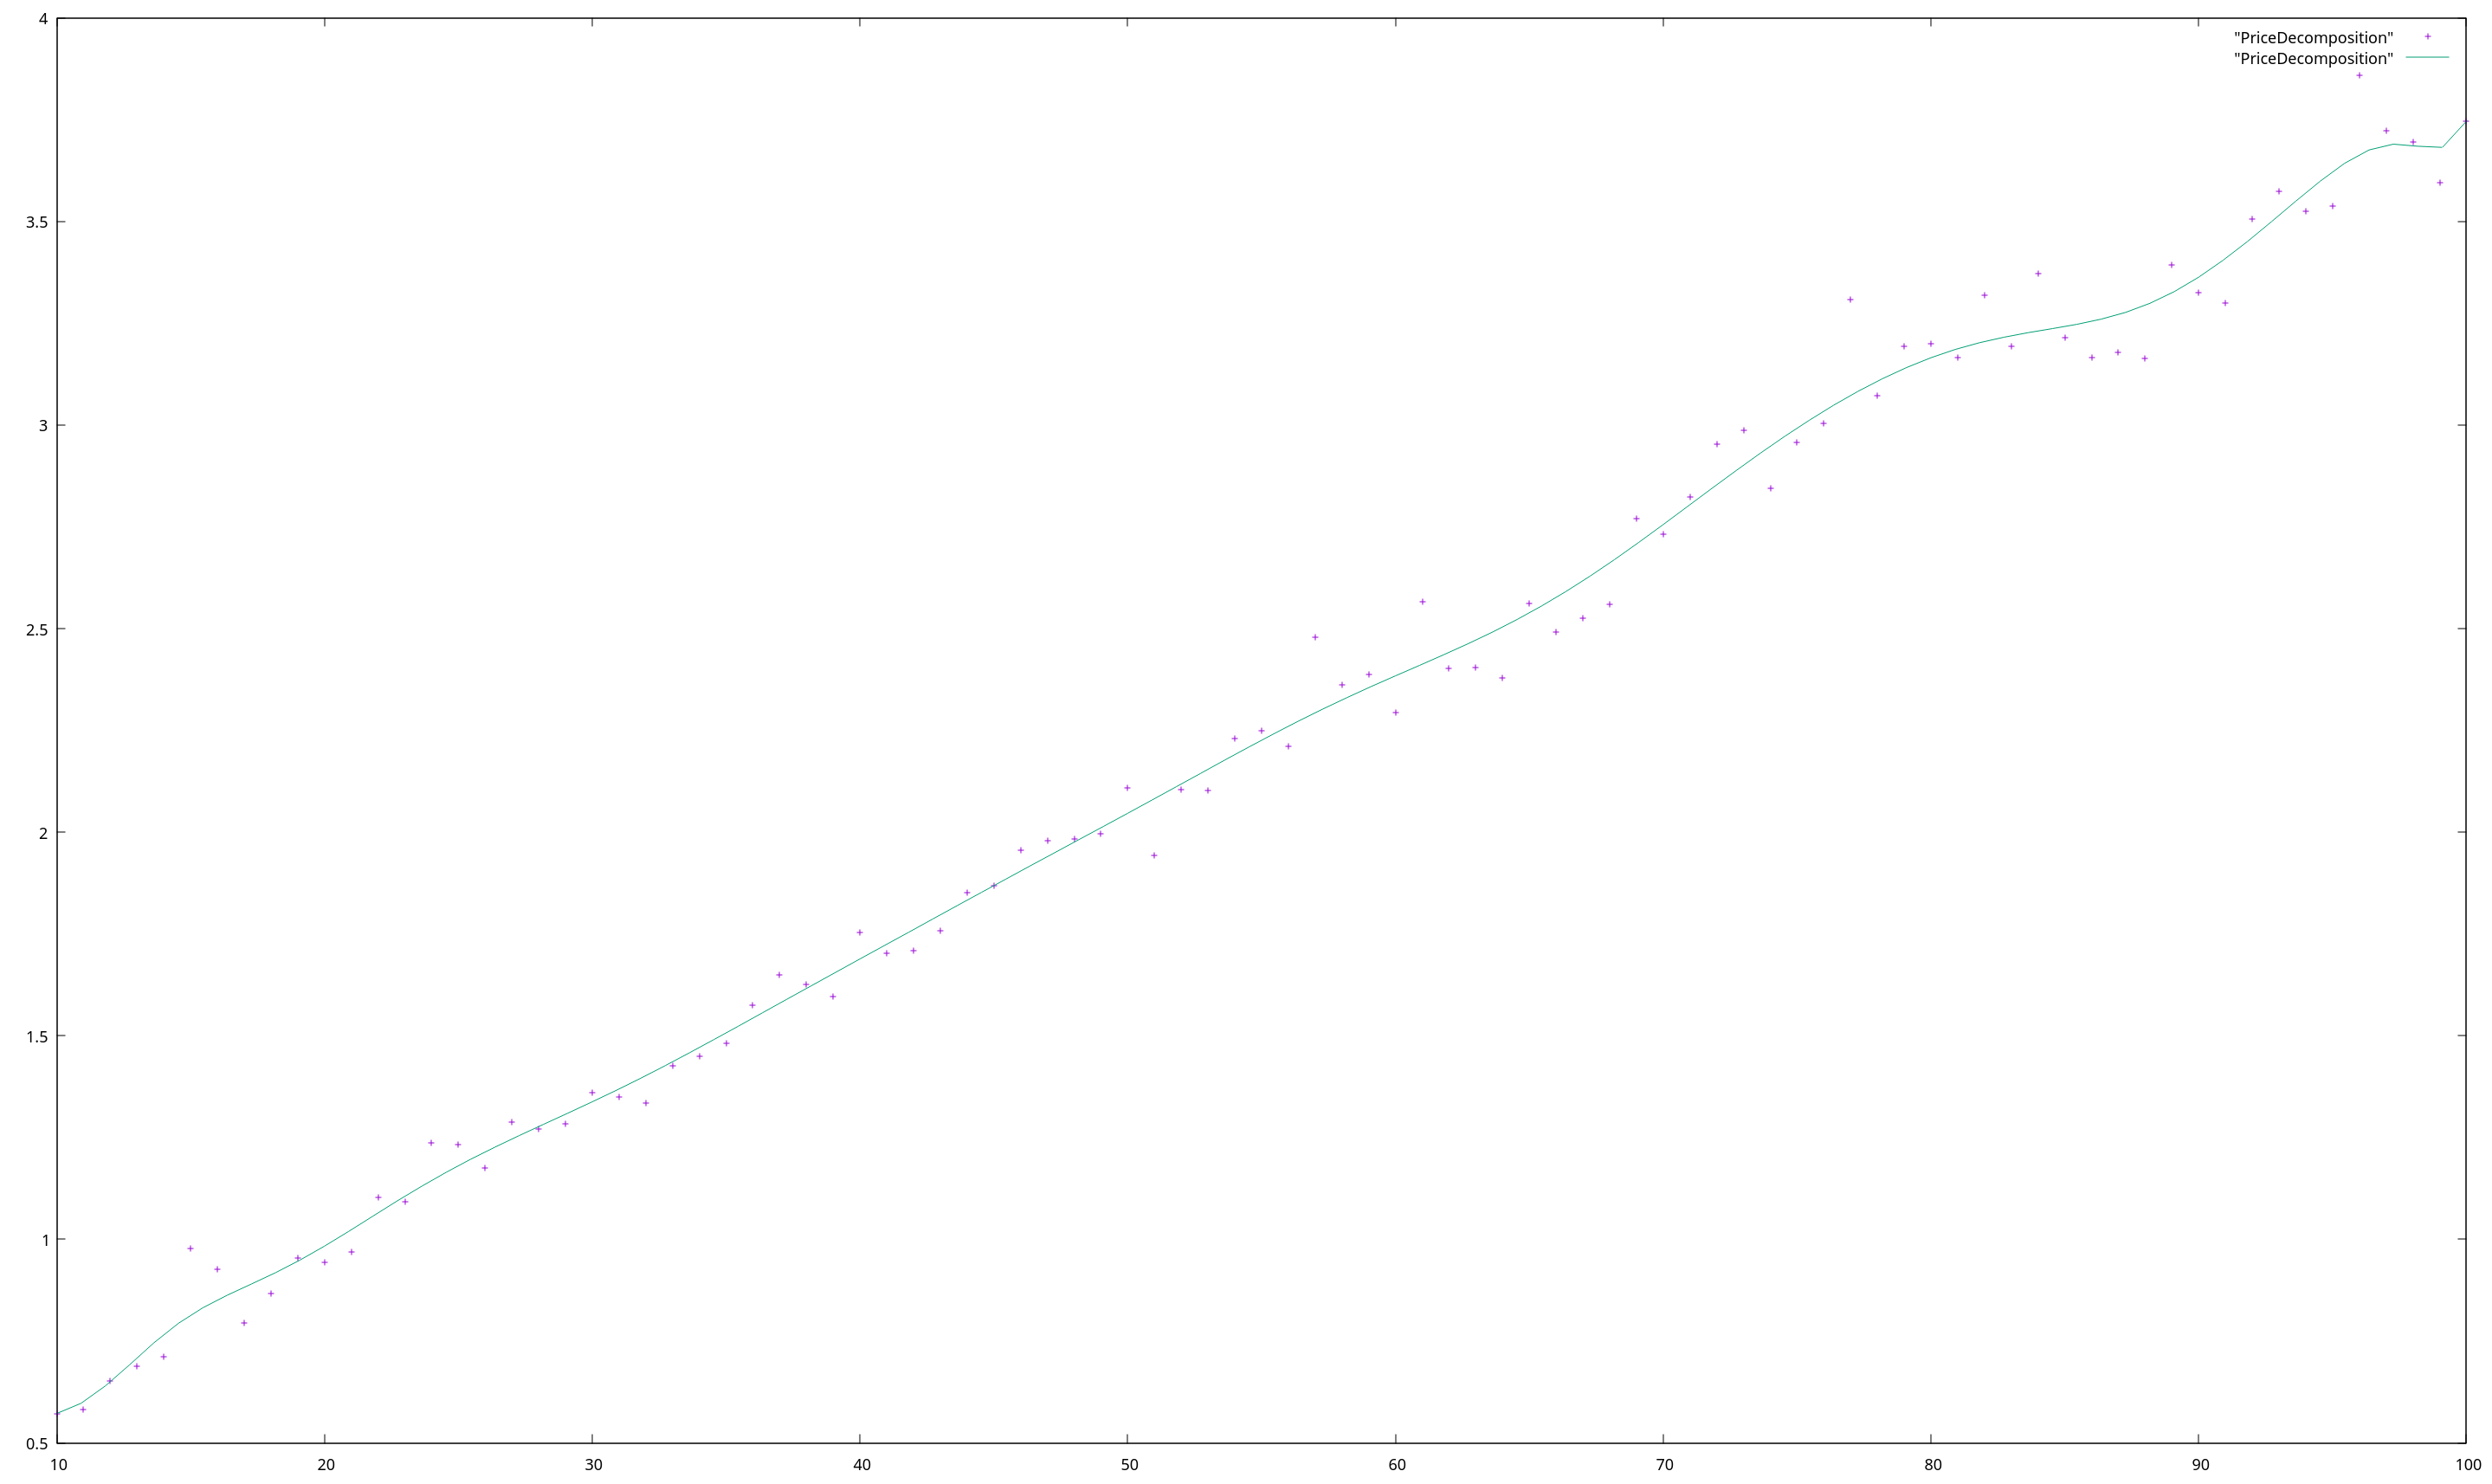
\includegraphics[width=\textwidth]{maxCost/PriceDecomposition}
\caption{Vývoj času výpočtu dekompozicí podle ceny (pro různou maximální cenu)}
\label{maxCost/PriceDecomposition}
\end{center}
\end{figure}

Graf pro heuristický algoritmus na obrázku \ref{maxCost/PriceToWeightRatio} je opět náhodný, opět jako v sekci \ref{maxWeight} se pohybuje kolem 0.14 milisekund a opět je náhodný.

\begin{figure}[H]
\begin{center}
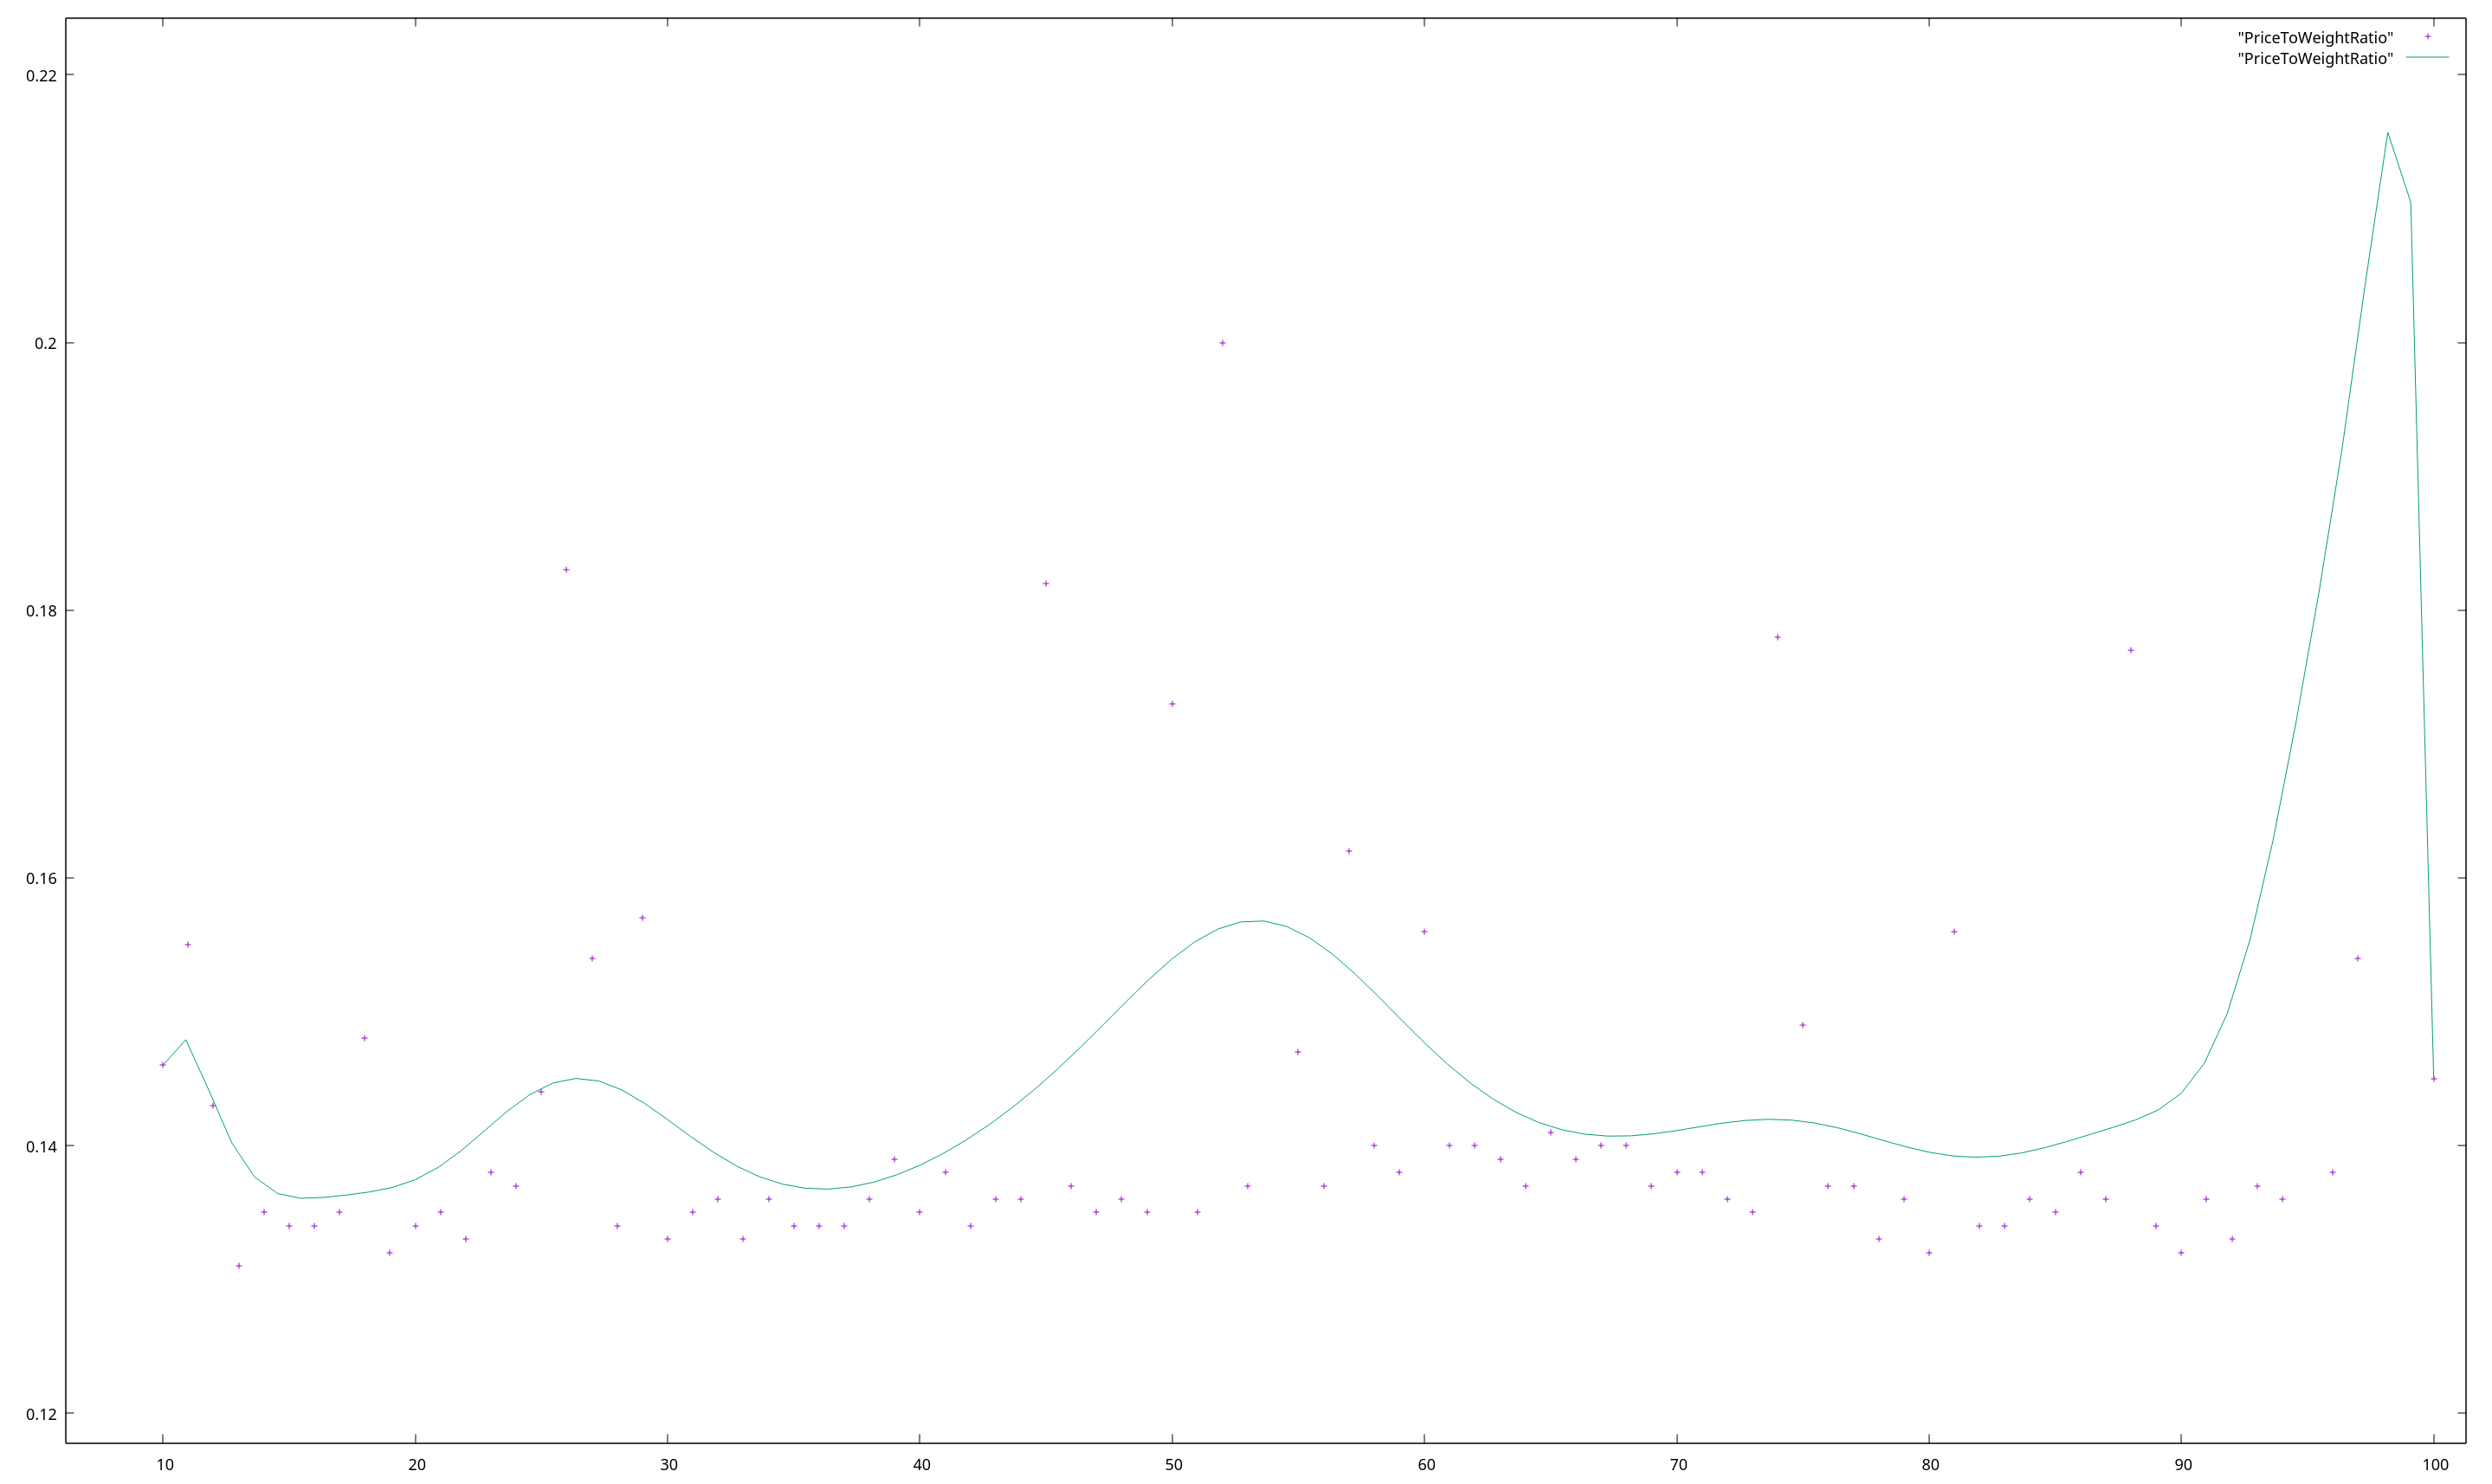
\includegraphics[width=\textwidth]{maxCost/PriceToWeightRatio}
\caption{Vývoj času výpočtu heuristikou (pro různou maximální cenu)}
\label{maxCost/PriceToWeightRatio}
\end{center}
\end{figure}

Vývoj relativní chyby na obrázku \ref{maxCost/PriceToWeightRatio-relerrs} je opět v zásadě lineární, s náhodnými odchylkami, pohybuje se okolo chyby 0.04, tak jako v sekci \ref{maxWeight}.

\begin{figure}[H]
\begin{center}
\includegraphics[width=\textwidth]{maxCost/PriceToWeightRatio-relerrs}
\caption{Vývoj relativní chyby výpočtu heuristikou (pro různou maximální cenu)}
\label{maxCost/PriceToWeightRatio-relerrs}
\end{center}
\end{figure}

Srovnání těchto metod z hlediska výpočetního času, je vidět na grafu \ref{maxCost/allExecTimes}. Je patrné, že jediná metoda, která vykazuje jasnou závislost na parametru maximální ceny je metoda dekompozice podle ceny. Ta je pro maximální cenu kolem 10 stejně efektivní jako metoda větví a hranic, kolem maximální ceny 50 je stejně efektivní jako hrubá síla, a pro vyšší ceny je dokonce méně efektivní než hrubá síla (pro toto zafixování parametrů, viz úvod).

\begin{figure}[H]
\begin{center}
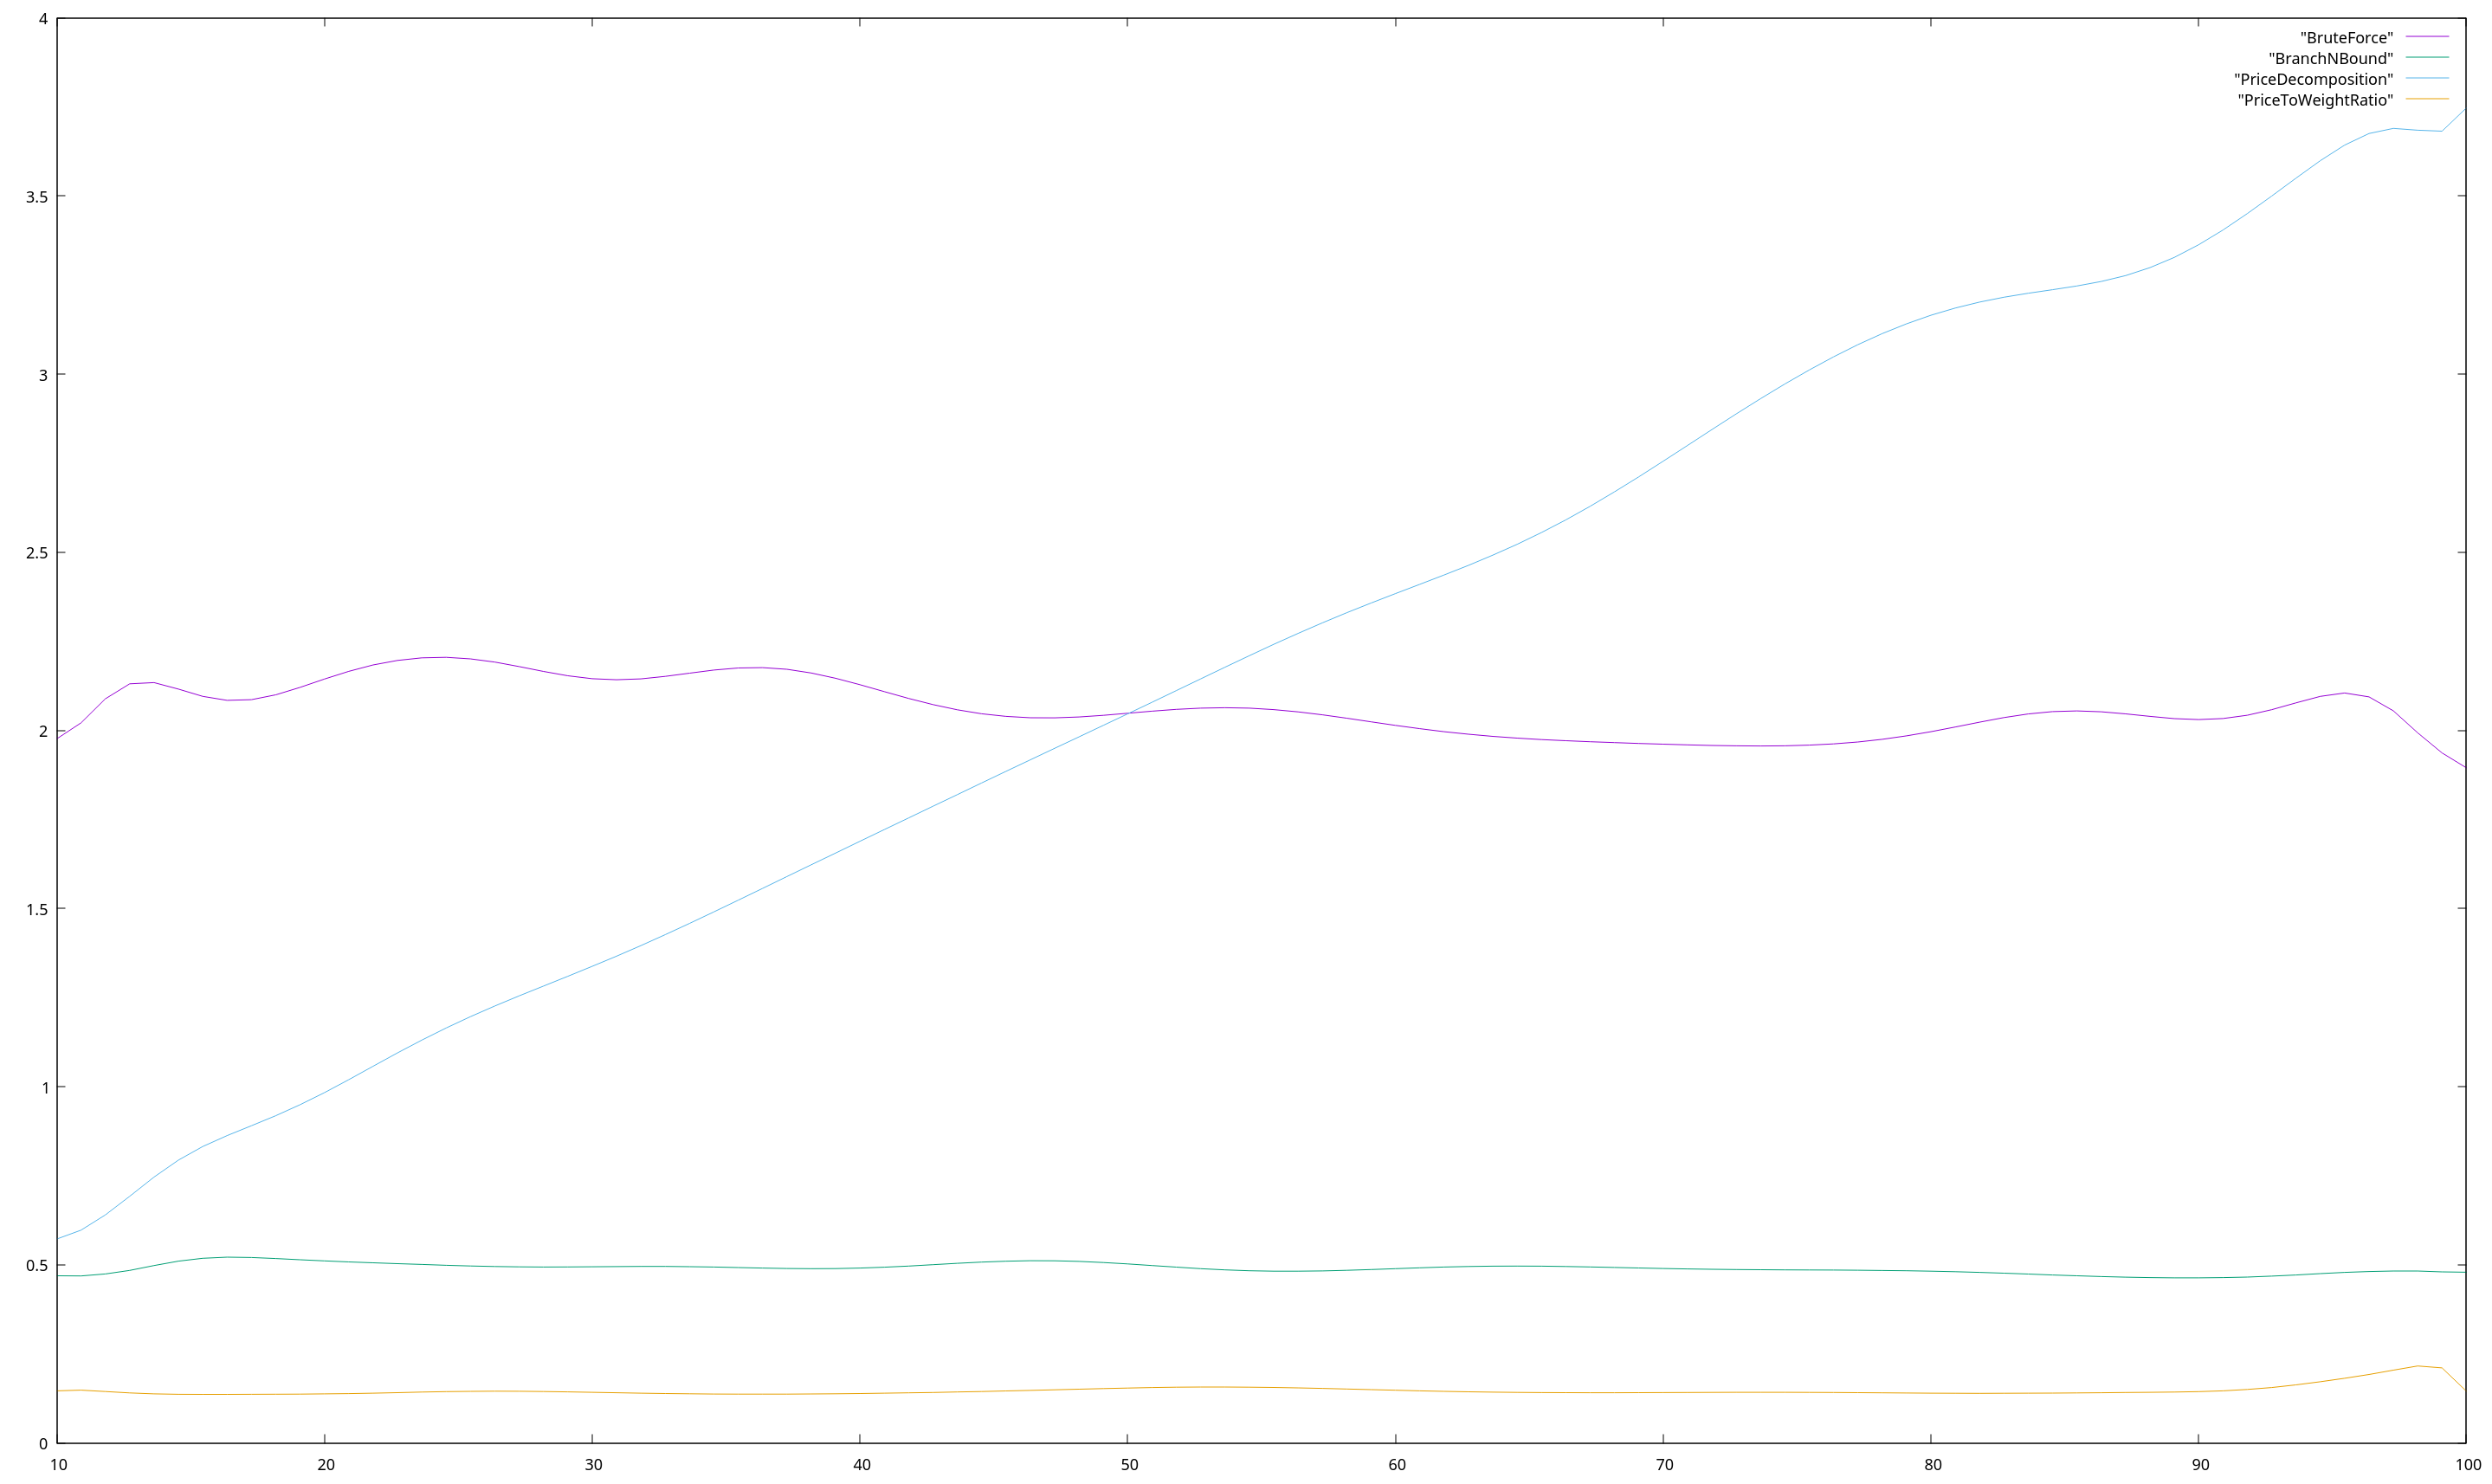
\includegraphics[width=\textwidth]{maxCost/allExecTimes}
\caption{Srovnání závislosti metod na maximální ceně}
\label{maxCost/allExecTimes}
\end{center}
\end{figure}









\section{Změna poměru kapacity batohu vůči celkové váze}

Další z nastavitelných parametrů je poměr mezi kapacitou batohu a sumární váze všech věcí, které do něj chceme umístit. Poměr 1.0 tedy znamená, že batoh pojme všechny věci a optimální řešení je takové, jehož vektor přidaných věcí je $1^n$, kde $n$ je počet věcí.

Tento parametr jsem měnil v rozmezí 0.01 až 1.00 se skokem 0.01. To znamená, že jsem získal 100 různých měření pro každých padesát instancí daných vlastností. 

V případě tohoto parametru jsem již očekával větší závislosti než v případě sekcí \ref{maxWeight} a \ref{maxCost}.

Graf závislosti času výpočtu hrubou silou na tomto poměru je zaznamenán na obrázku \ref{ratio/BruteForce}. Čas výpočtu přibližně lineárně roste, je ale prohnut mírně do písmena S, kde rychleji roste uprostřed rozmezí, kolem poměru 0.5. Zde je velmi patrná závislost, která vychází z drobného vylepšení tohoto algoritmu, které ořezává stavový prostor, jakmile je batoh plný. Pokud se tedy téměř všechny věci do batohu vejdou, stavový prostor není ořezáván a čas výpočtu je delší.

\begin{figure}[H]
\begin{center}
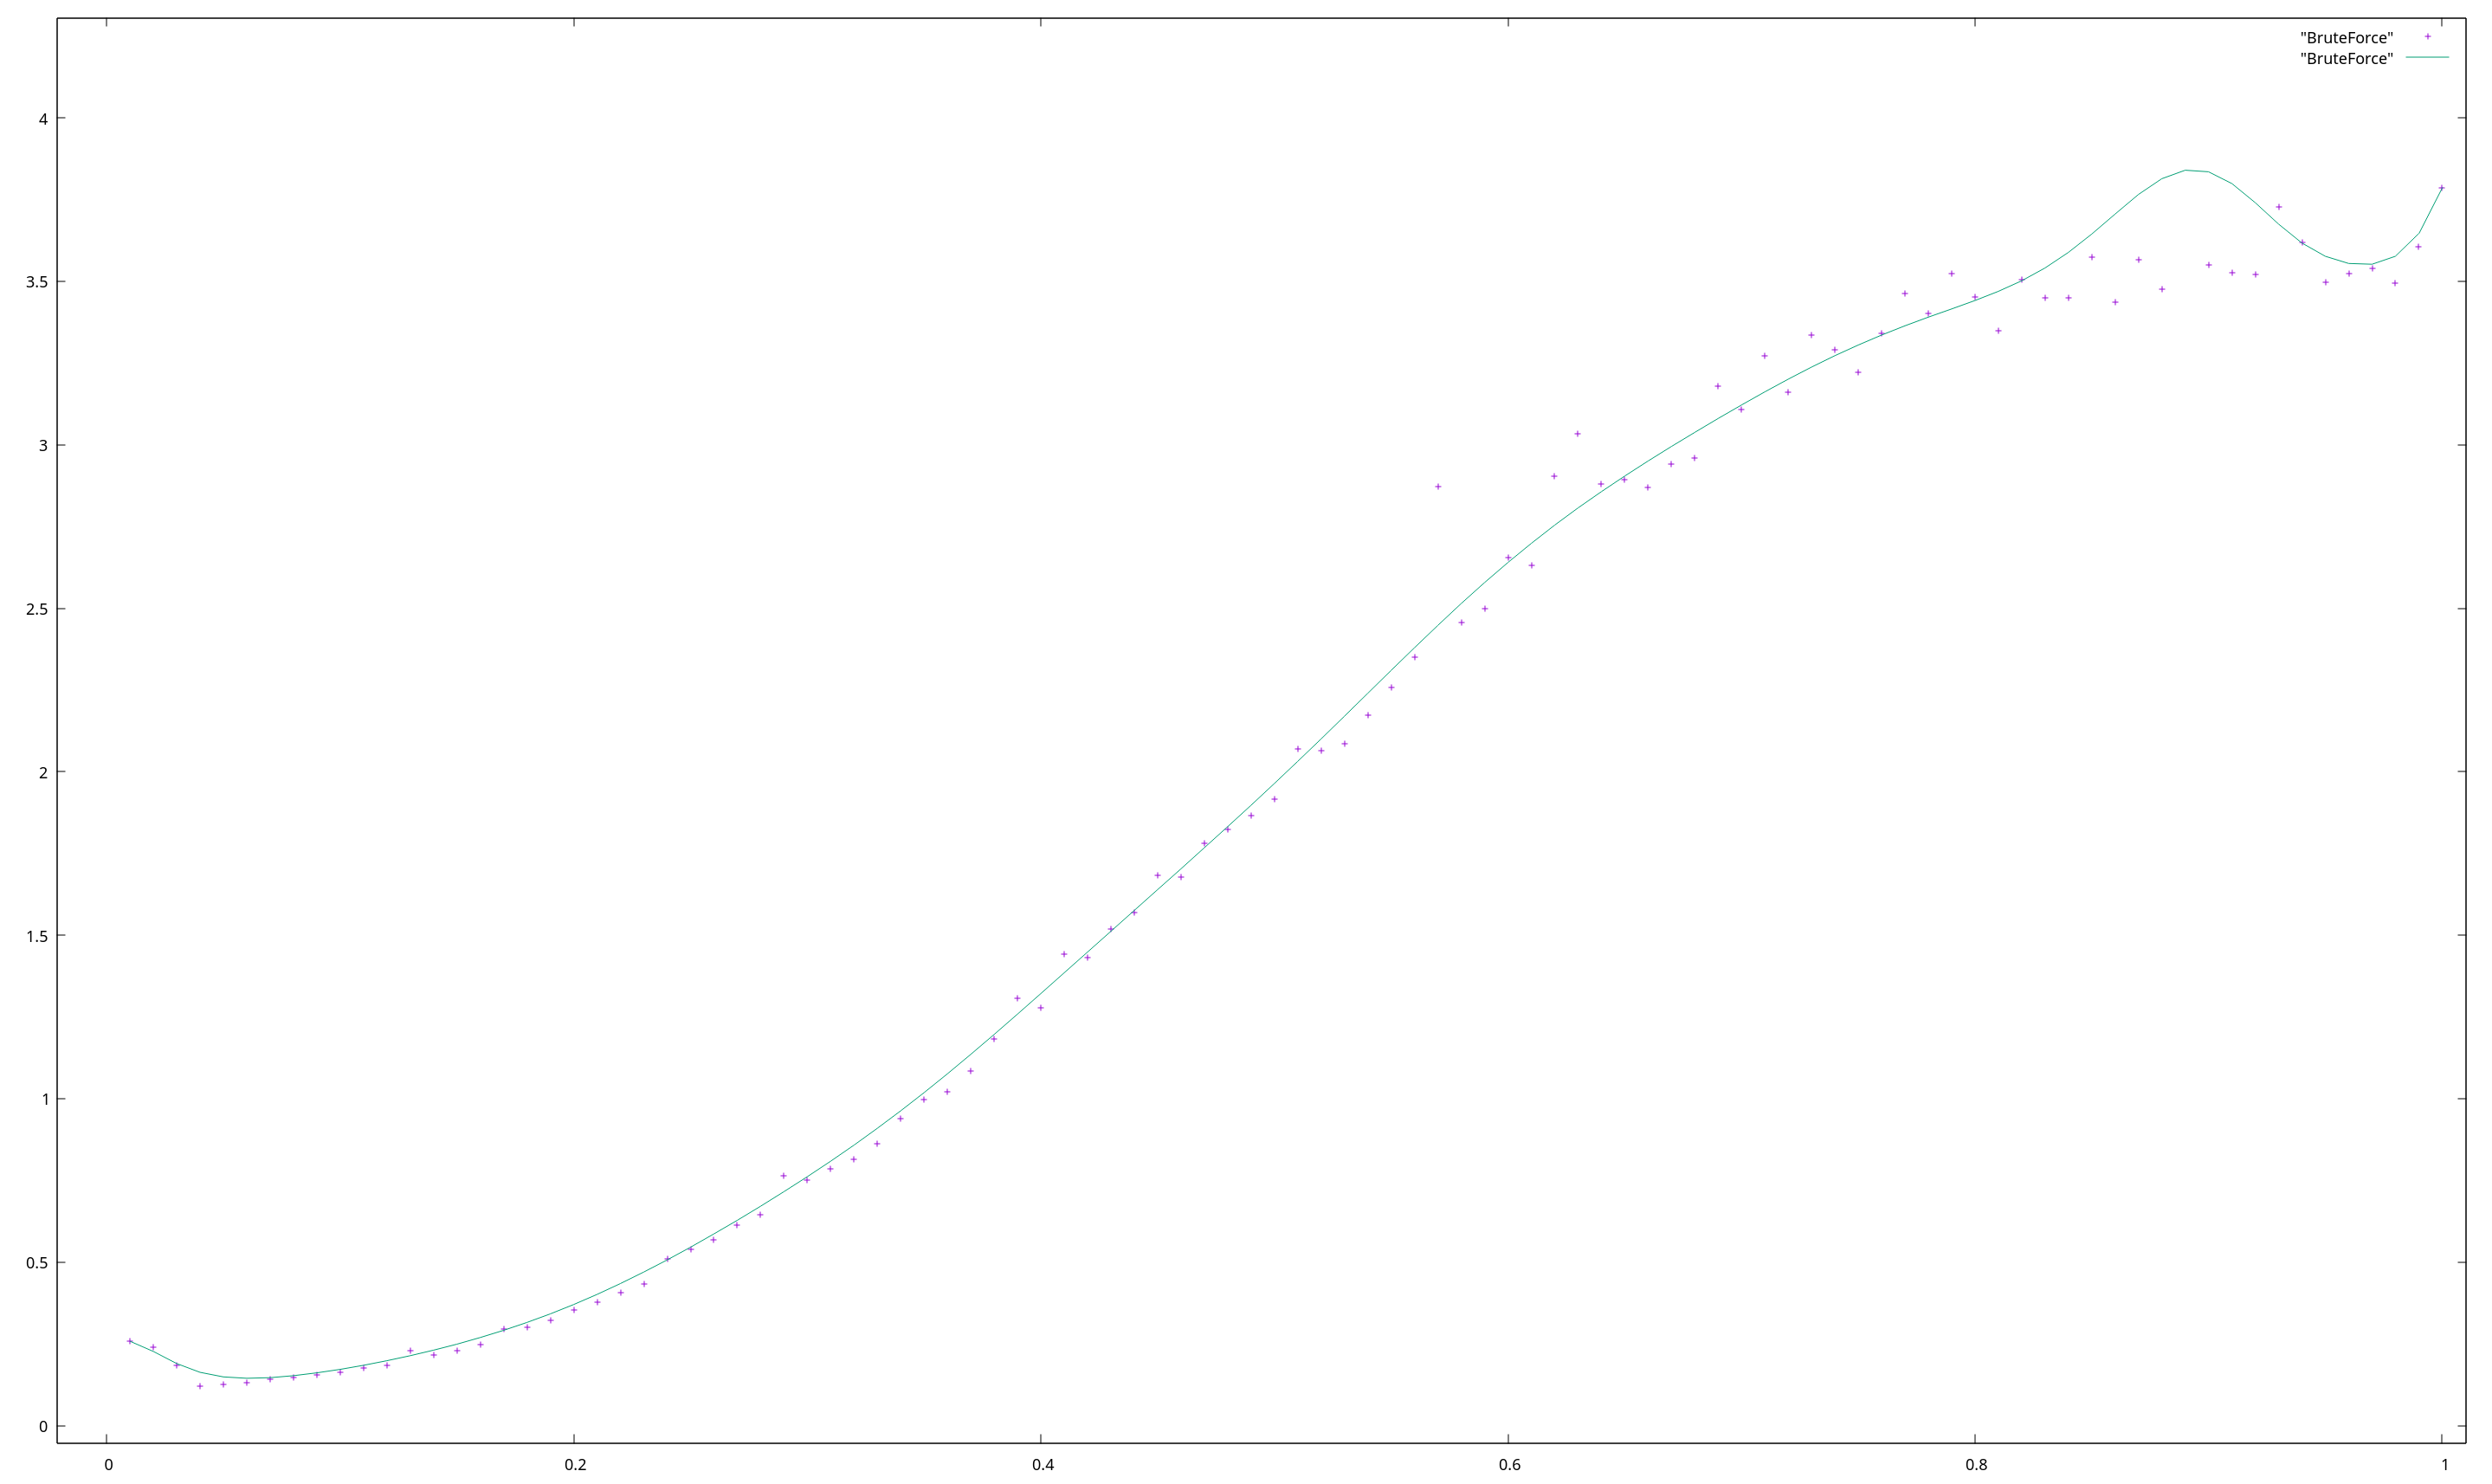
\includegraphics[width=\textwidth]{ratio/BruteForce}
\caption{Vývoj času výpočtu hrubou silou (pro různý poměr kapacity a váhy)}
\label{ratio/BruteForce}
\end{center}
\end{figure}

Závislost času výpočtu metodou větví a hranic je na obrázku \ref{ratio/BranchNBound}. Tento graf je zajímavý. Má tvar podobný Gaussově křivce. Nejdéle trvá výpočet pro přibližně poloviční poměr. Tento algoritmus je rozšířením řešení hrubou silou, kde graf byl rostoucí (obr. \ref{ratio/BruteForce}). Tedy máme přibližně lineárně rostoucí graf jako zdroj, a další ořezávání v tomto algoritmu graf čím dál více ohýbá směrem dolů. Jinými slovy, ořezy jsou čím dál větší. To odpovídá, protože při větším poměru se do batohu vejde více věcí a stavový prostor je méně prořezaný. 

\begin{figure}[H]
\begin{center}
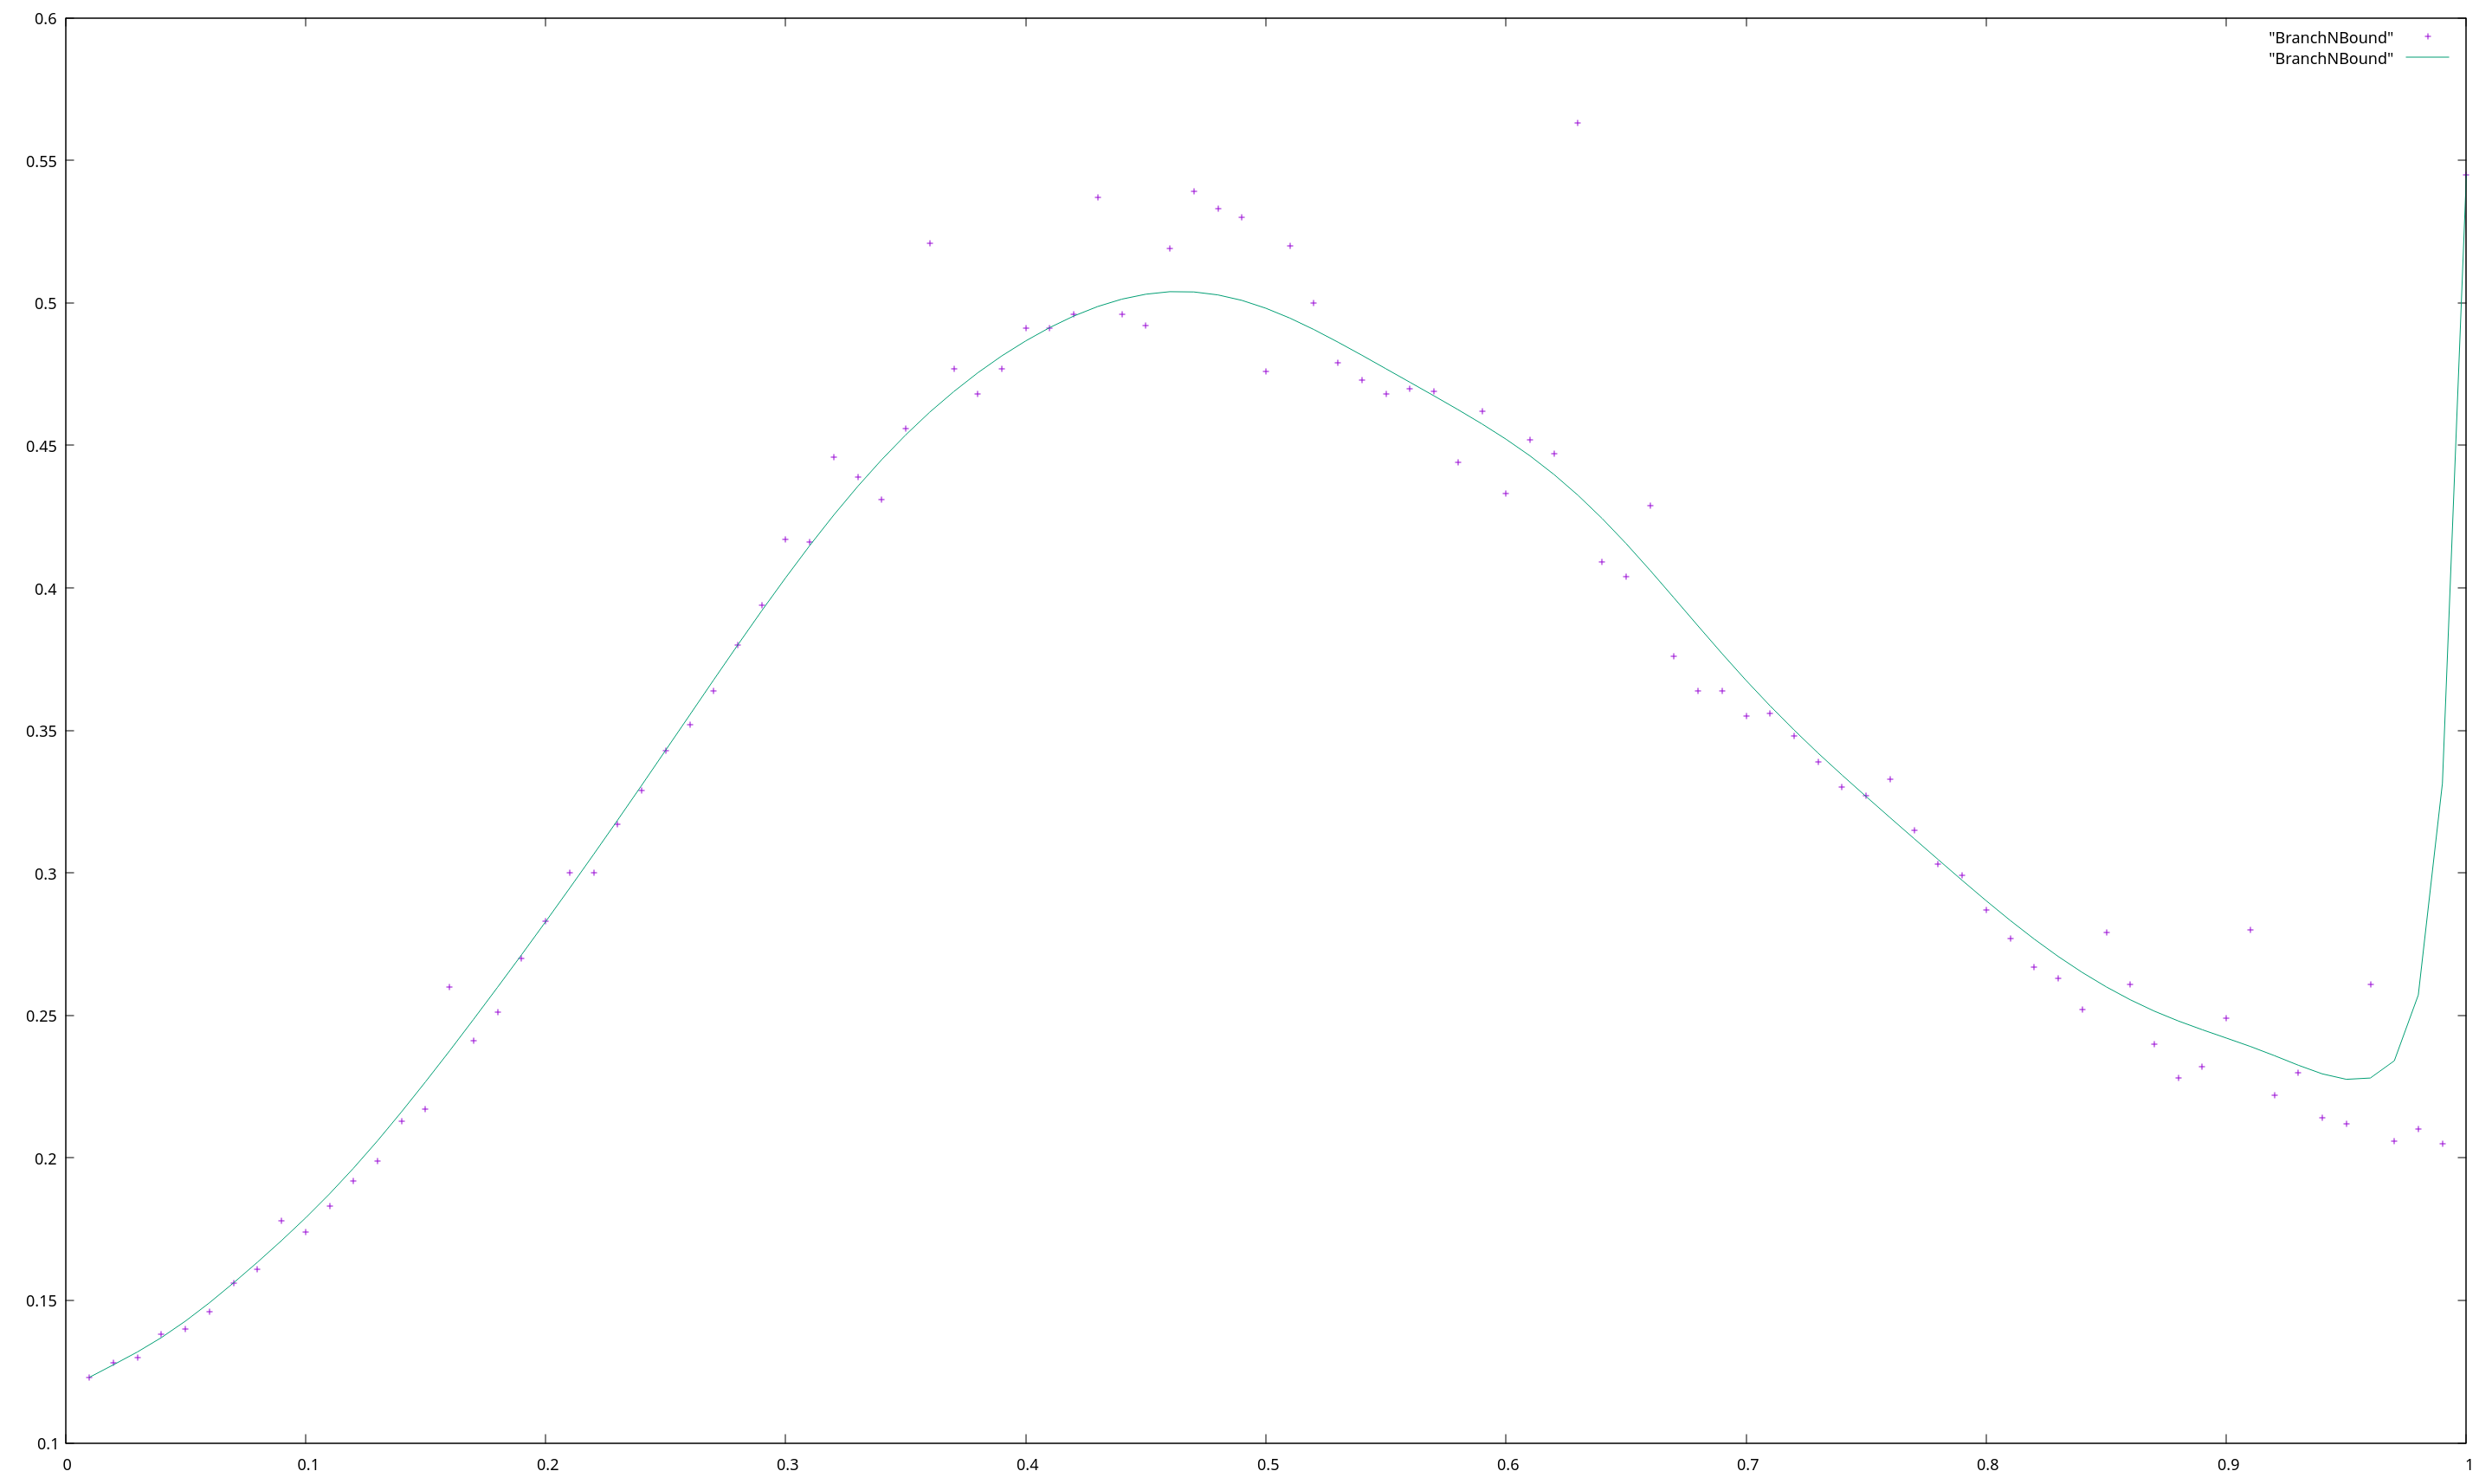
\includegraphics[width=\textwidth]{ratio/BranchNBound}
\caption{Vývoj času výpočtu metodou větví a hranic (pro různý poměr kapacity a váhy)}
\label{ratio/BranchNBound}
\end{center}
\end{figure}

Závislost času výpočtu dekompozicí podle ceny je naopak dle grafu \ref{ratio/PriceDecomposition} mizivá. Tabulku o velikosti $n*C$ poměr kapacity a váhy nijak nemění.

\begin{figure}[H]
\begin{center}
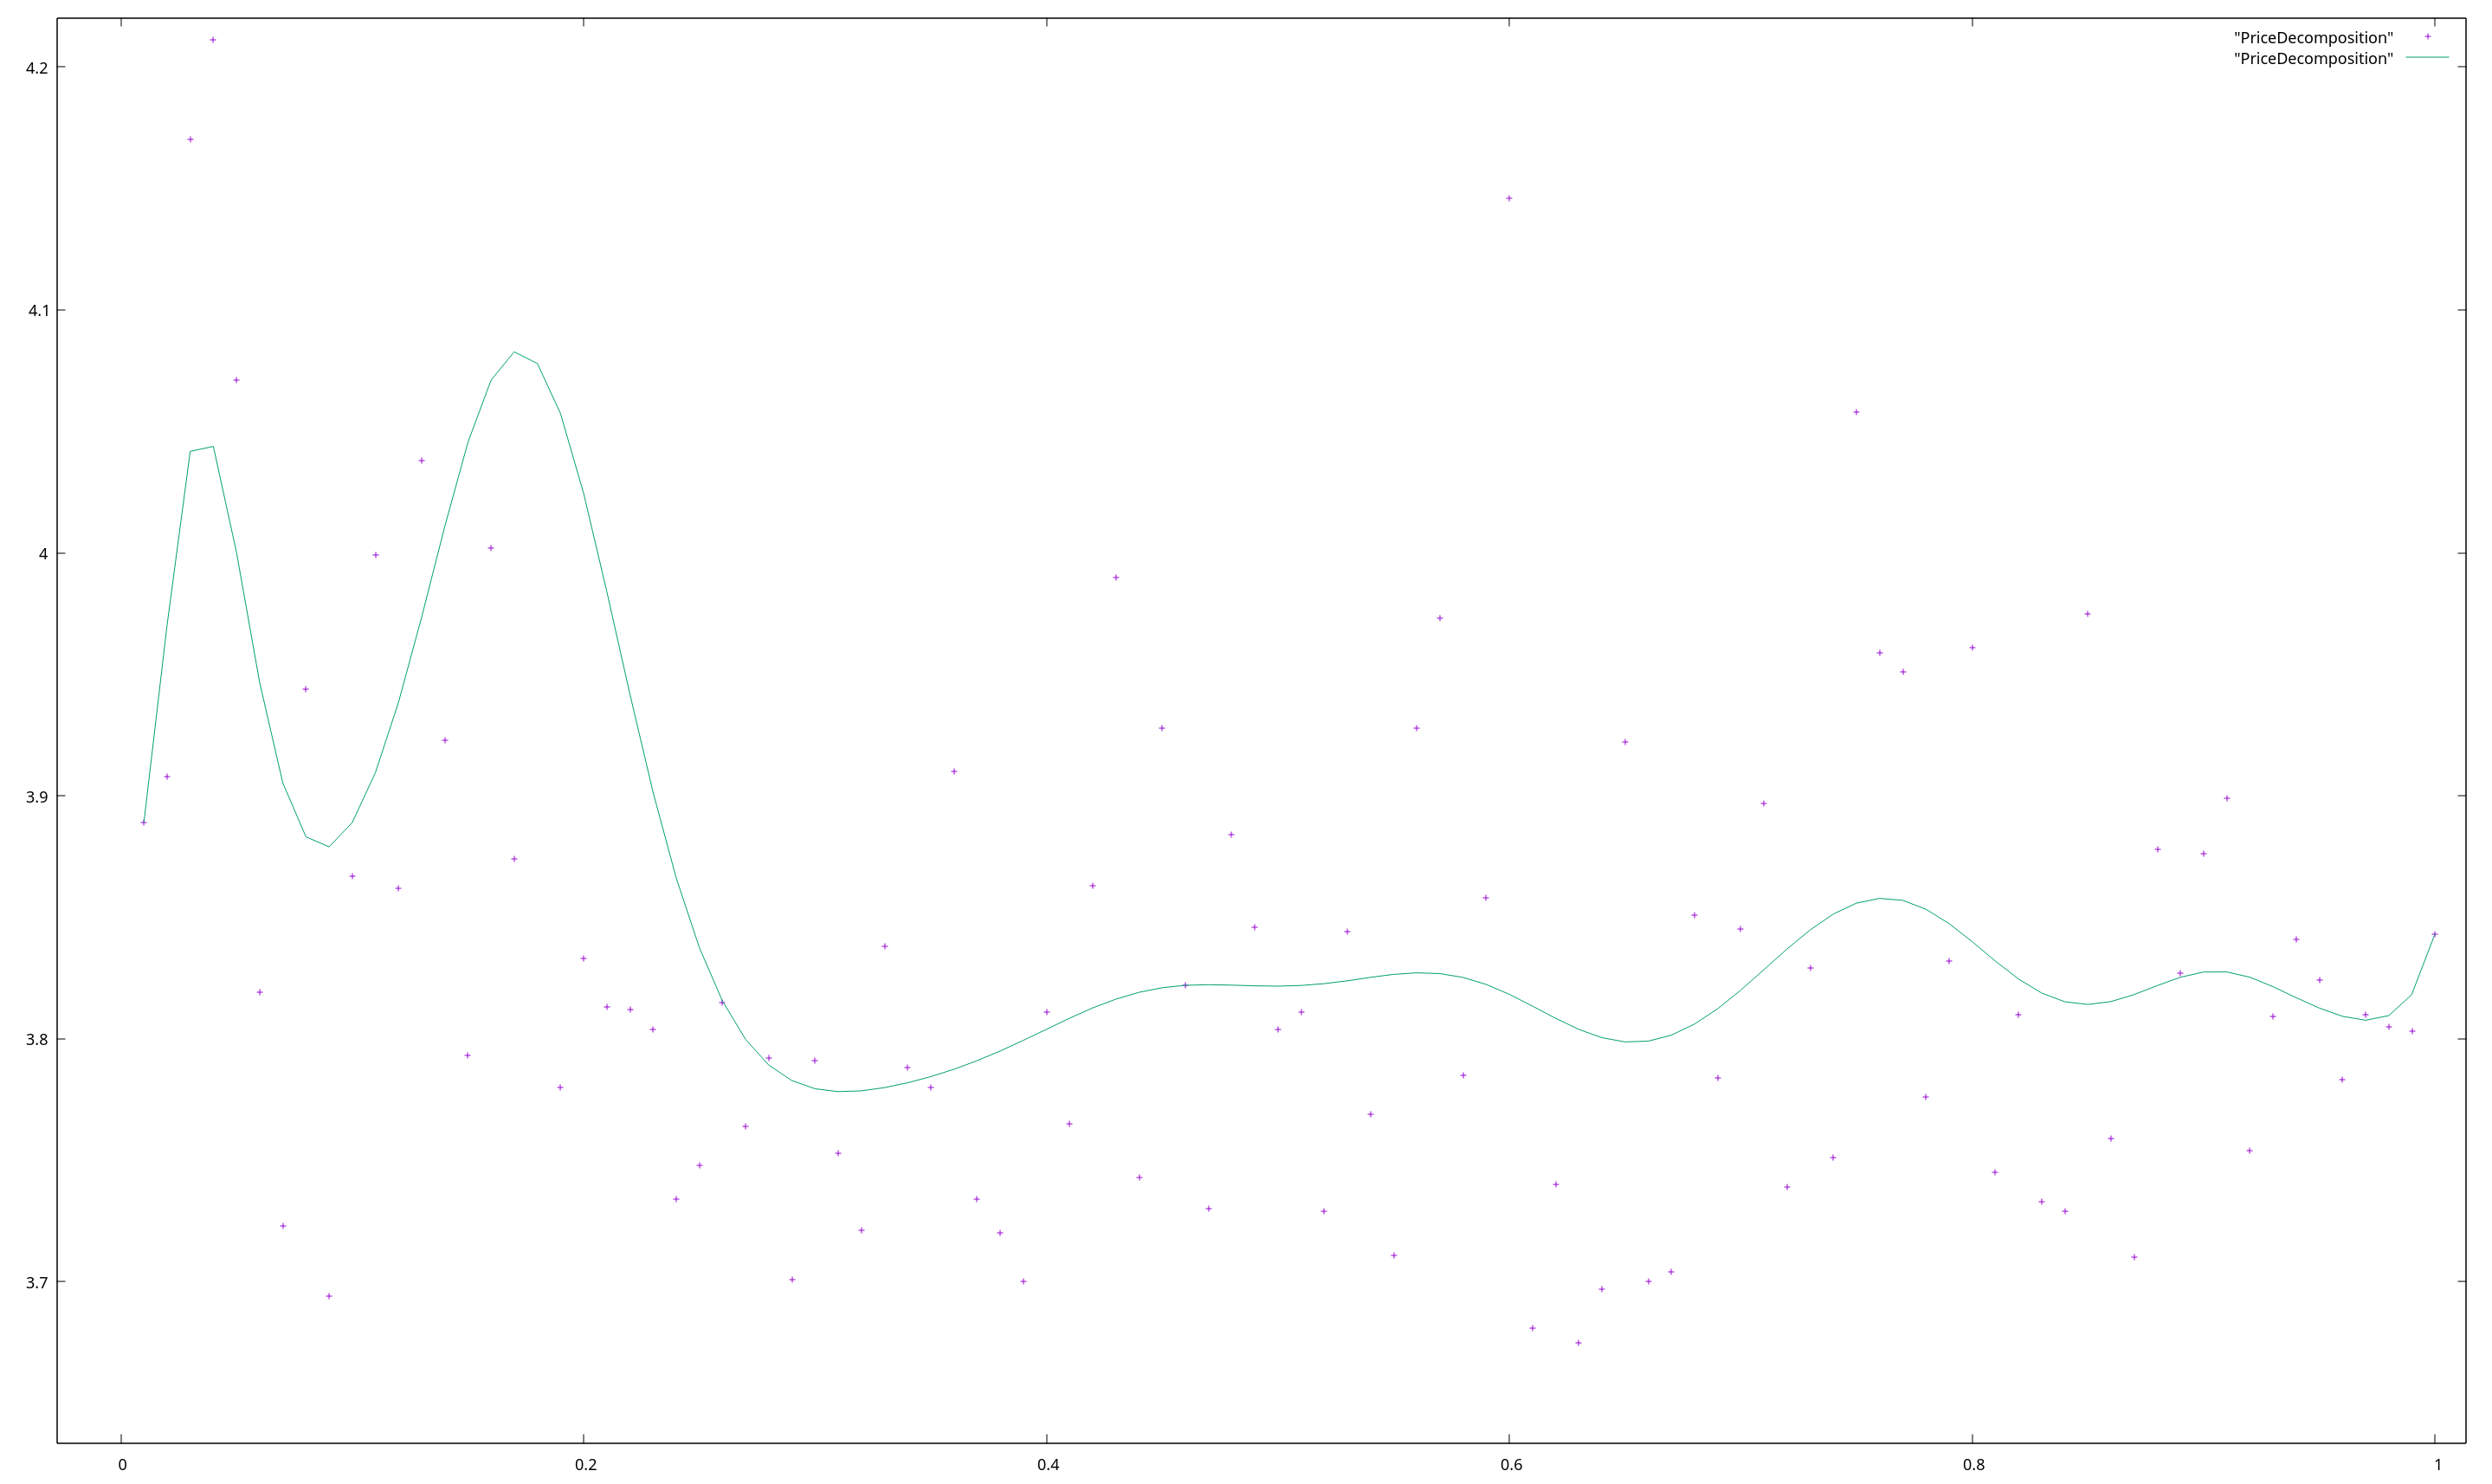
\includegraphics[width=\textwidth]{ratio/PriceDecomposition}
\caption{Vývoj času výpočtu dekompozicí podle ceny (pro různý poměr kapacity a váhy)}
\label{ratio/PriceDecomposition}
\end{center}
\end{figure}

Graf závislosti pro heuristickou metodu na obrázku \ref{ratio/PriceToWeightRatio} je přibližně lineárně rostoucí. Tato heuristická metoda prochází prostor v zásadě lineárně, vždy vybere jednoznačně další stav, do kterého přejít, dokud v některém neskončí. Při větších váhách vůči kapacitě se batoh naplní dříve.

\begin{figure}[H]
\begin{center}
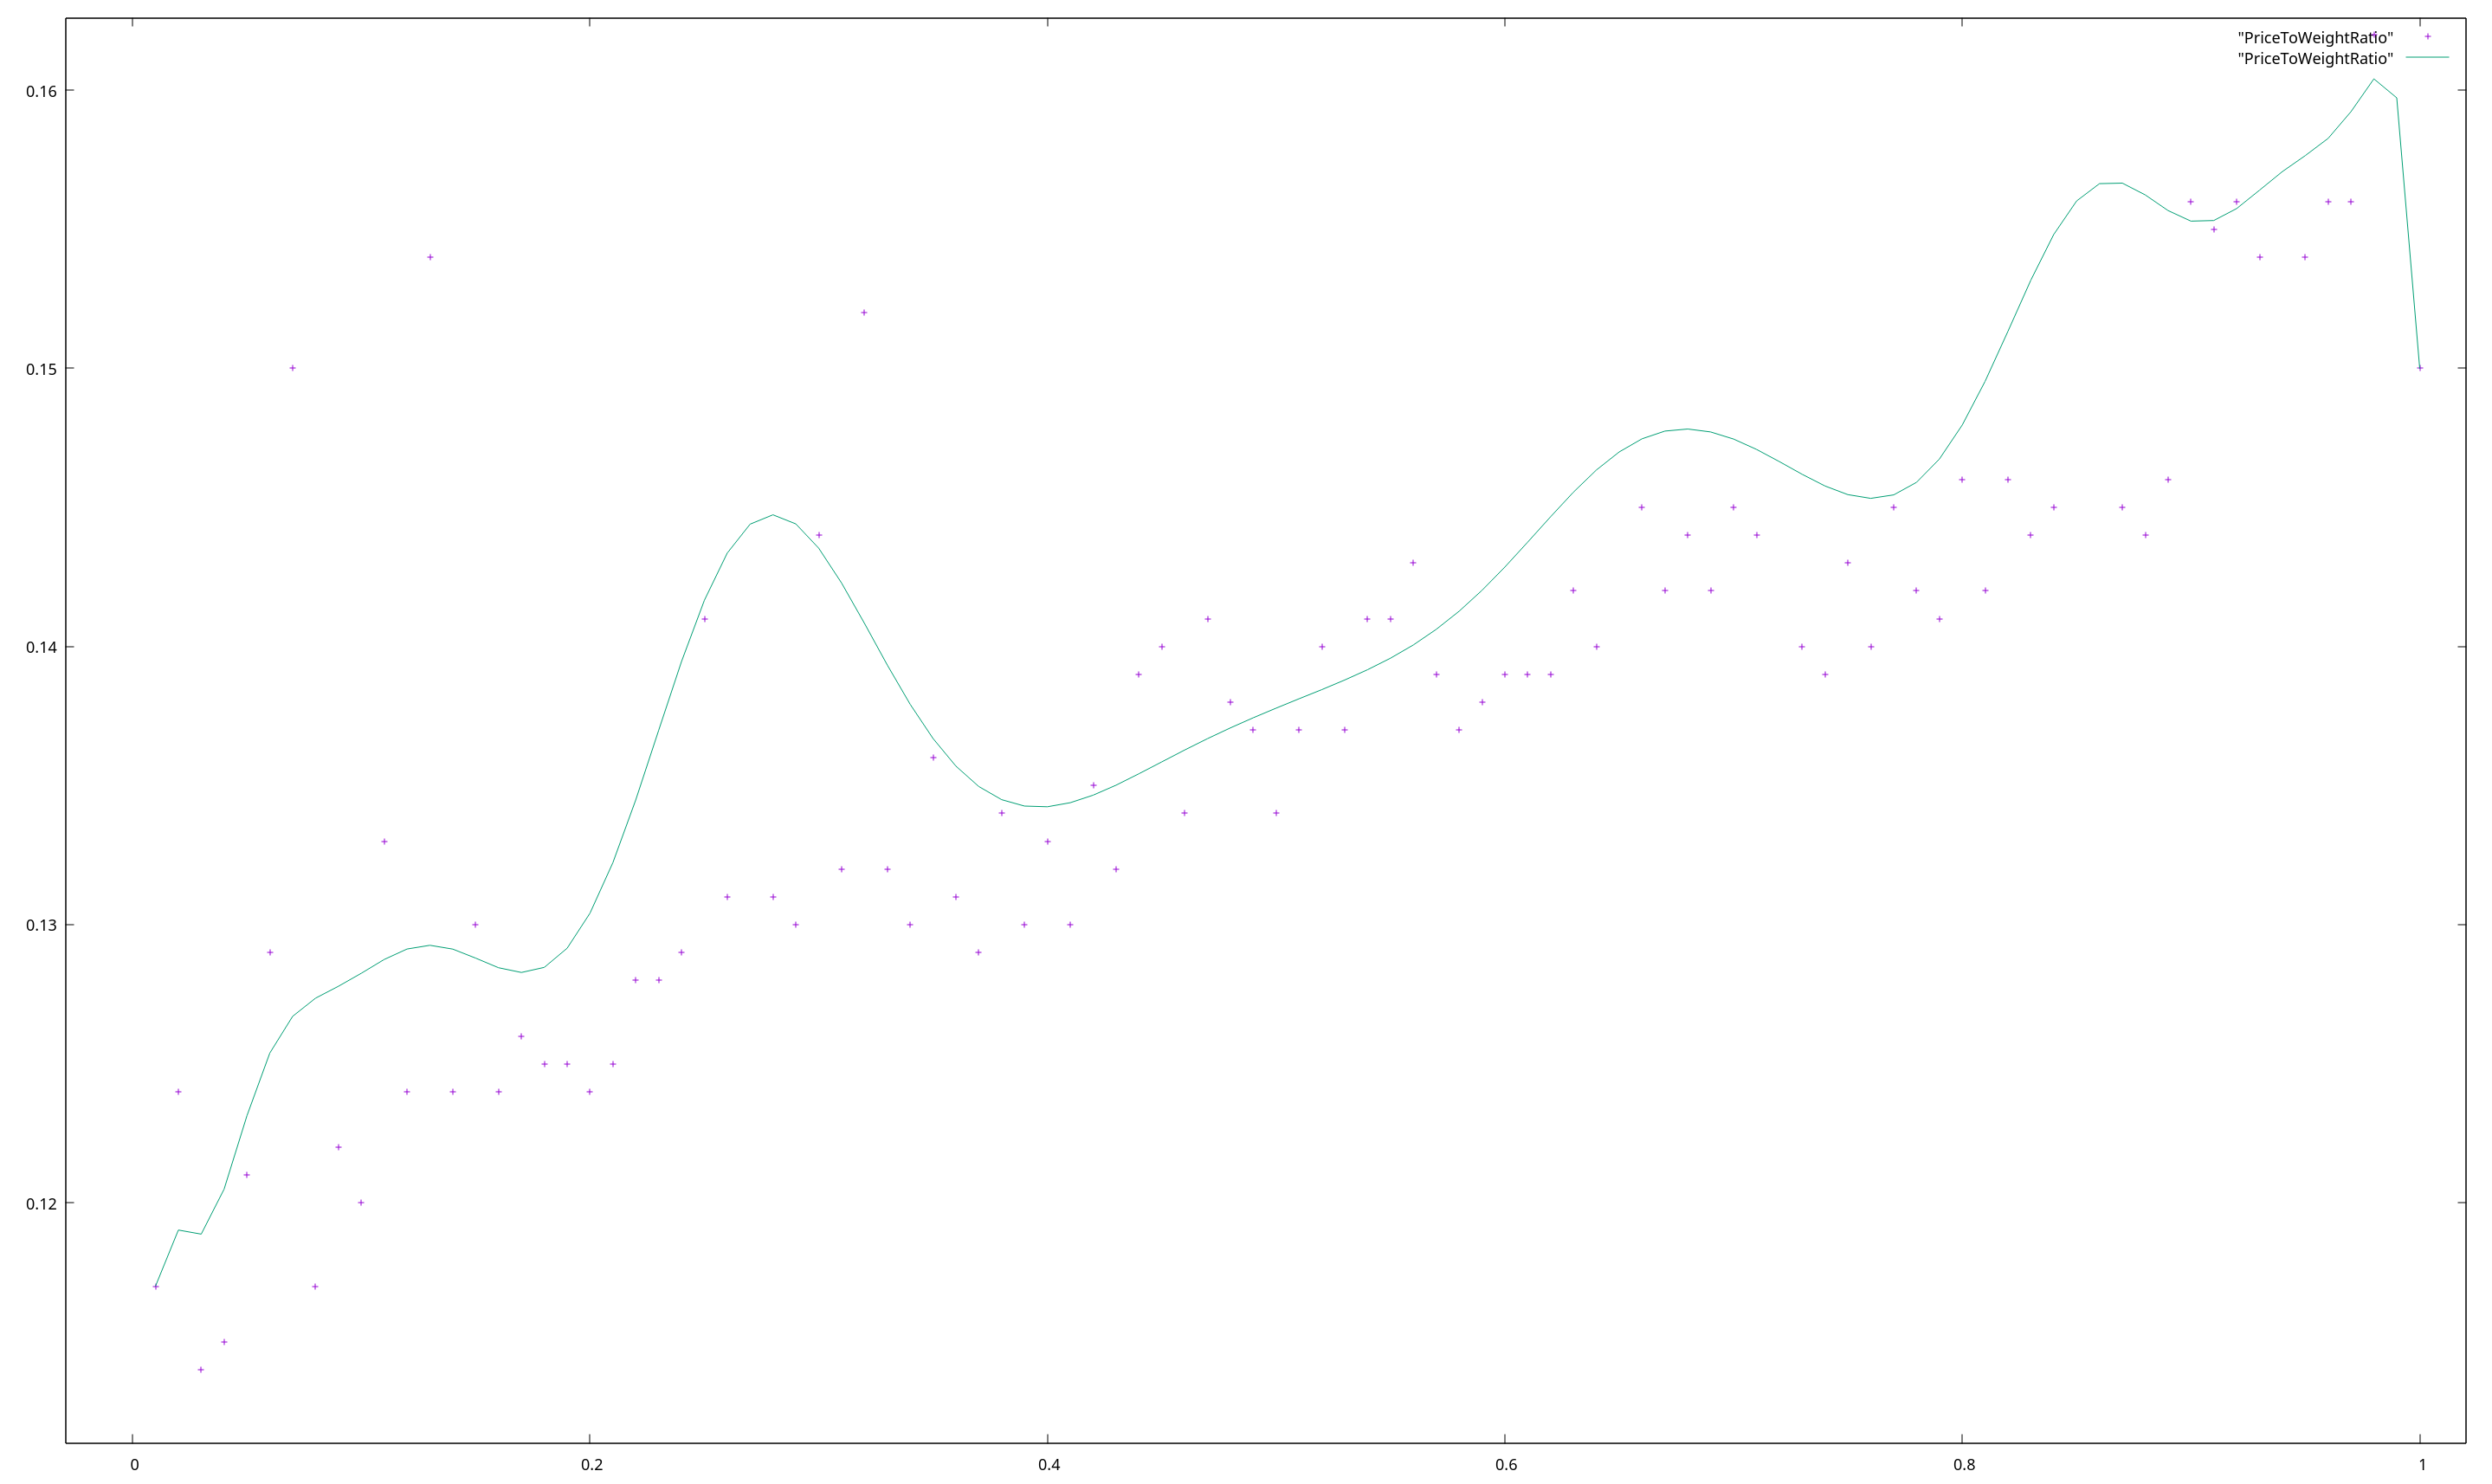
\includegraphics[width=\textwidth]{ratio/PriceToWeightRatio}
\caption{Vývoj času výpočtu heuristikou (pro různý poměr kapacity a váhy)}
\label{ratio/PriceToWeightRatio}
\end{center}
\end{figure}

Vývoj relativní chyby dle grafu \ref{ratio/PriceToWeightRatio-relerrs} klesá asymptoticky k nule. Důvod je zřejmý, pokud se vejdou do batohu všechny věci, je jedno, kterou vybereme první, výsledek bude vždy optimální. Pokud se naopak vejde jen jedna, je obtížné trefit ji jen na základě slabé heuristiky napoprvé, proto je chyba větší.

\begin{figure}[H]
\begin{center}
\includegraphics[width=\textwidth]{ratio/PriceToWeightRatio-relerrs}
\caption{Vývoj relativní chyby výpočtu heuristikou (pro různý poměr kapacity a váhy)}
\label{ratio/PriceToWeightRatio-relerrs}
\end{center}
\end{figure}

Srovnání těchto metod z hlediska výpočetního času je vidět v grafu \ref{ratio/allExecTimes}. Na parametru poměru kapacity a sumární váhy závisí především metoda hrubé síly. Metoda větví a hranic je o něco méně efektivní okolo polovičního poměru.

\begin{figure}[H]
\begin{center}
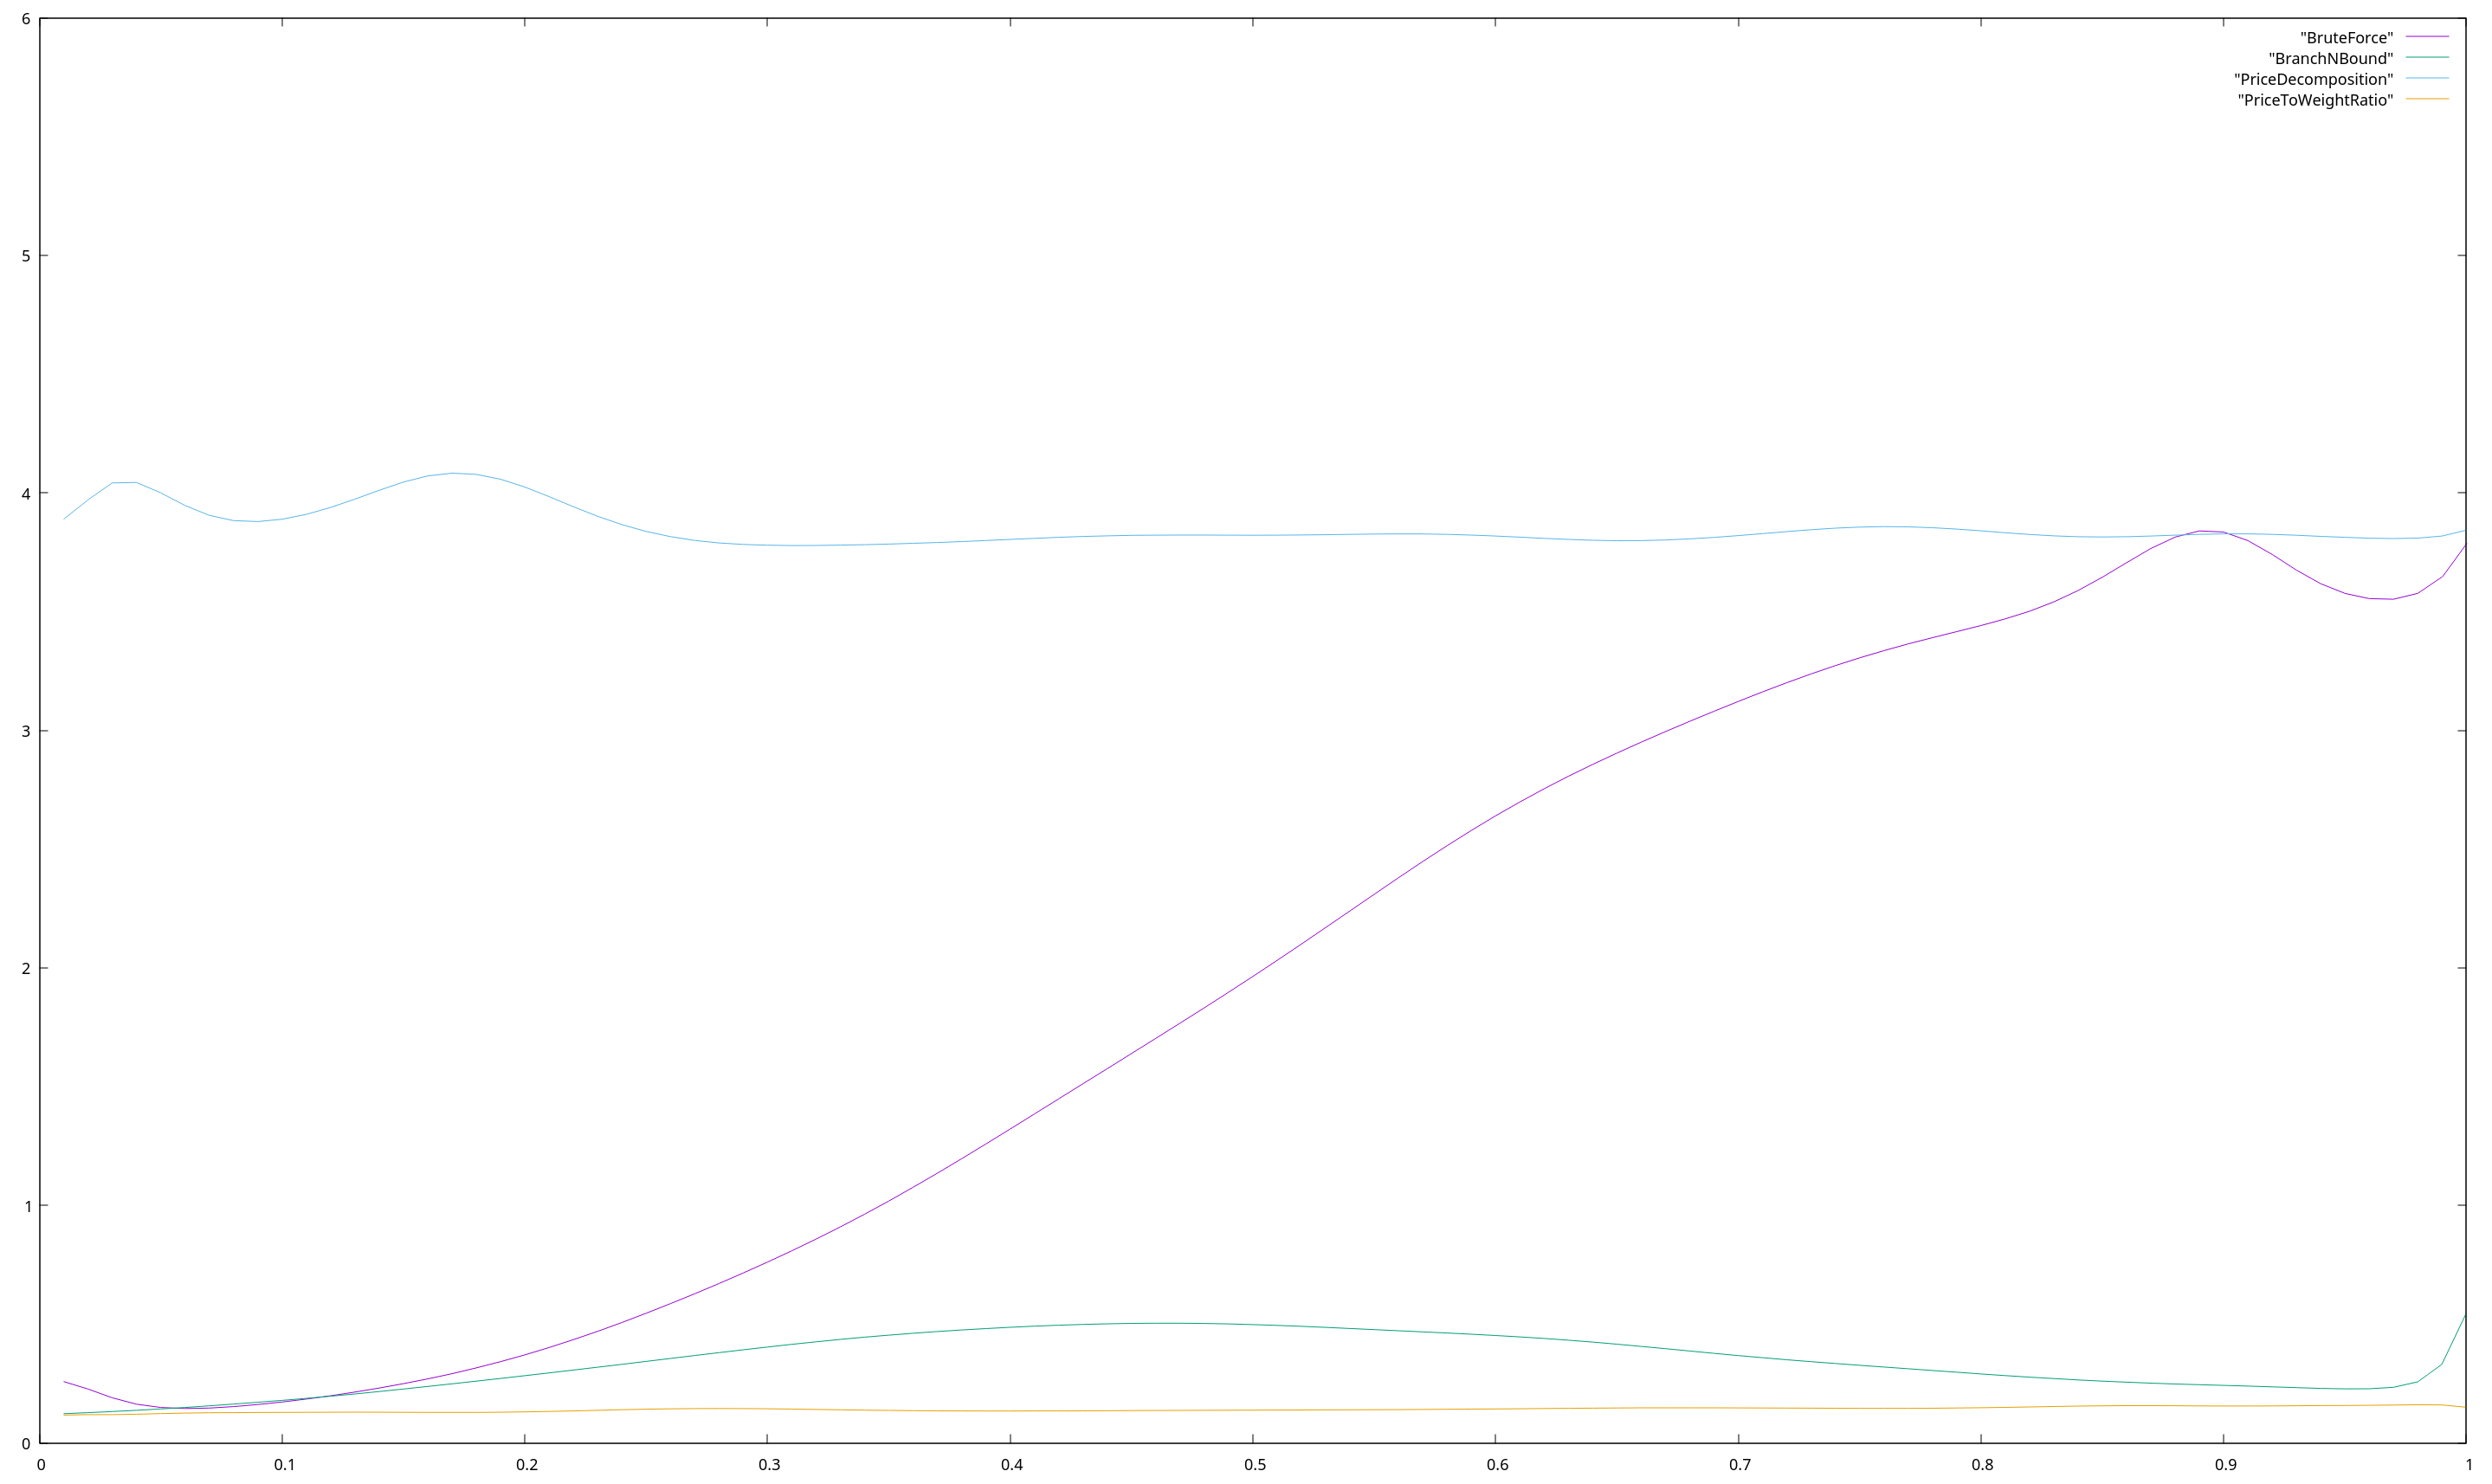
\includegraphics[width=\textwidth]{ratio/allExecTimes}
\caption{Srovnání závislosti metod na poměru kapacity a sumární váhy}
\label{ratio/allExecTimes}
\end{center}
\end{figure}







\section{Změna exponentu}

Dalším nastavitelným parametrem, který by mohl mít vliv na dobu výpočtu, je exponent, který figuruje v pravděpodobnosti, že bude do instance zařazena vygenerovaná věc, která má určitou váhu. Jedna možnost je preferovat malé věci, druhá možnost je preferovat velké věci. V obou případech hraje roli tento exponent.



\subsection{Převaha malých věcí}

Rozhodneme-li se pro převahu malých věcí, má exponent roli $k$ ve vzorci pro pravděpodobnost, že určitá věc bude zahrnuta do instance, takovouto: $1/w^k$. Tedy pro větší exponent bude pravděpodobnost zařazení věci se stejnou váhou menší a bude dávána přednost čím dál menším věcem.

Tento exponent jsem zvolil měnit v rozmezí 0.1 a 4.0 se skokem 0.1. To znamená, že jsem naměřil 40 výsledků, každý provedený na 50 instancích daných vlastností. V případě exponentu většího než 4.0 jsem pozoroval přílišné zpomalení generátoru instancí, které nijak nesouvisí s řešením problému batohu.

Závislost času výpočtu hrubou silou na tomto exponentu pro převahu malých věcí je vidět v grafu \ref{exp/small/BruteForce}. Graf se zdá být dosti náhodný. Je to proto, že metoda hrubé síly prochází prostor v zásadě celý, nehledě na to, zda jsou váhy větší či menší.

\begin{figure}[H]
\begin{center}
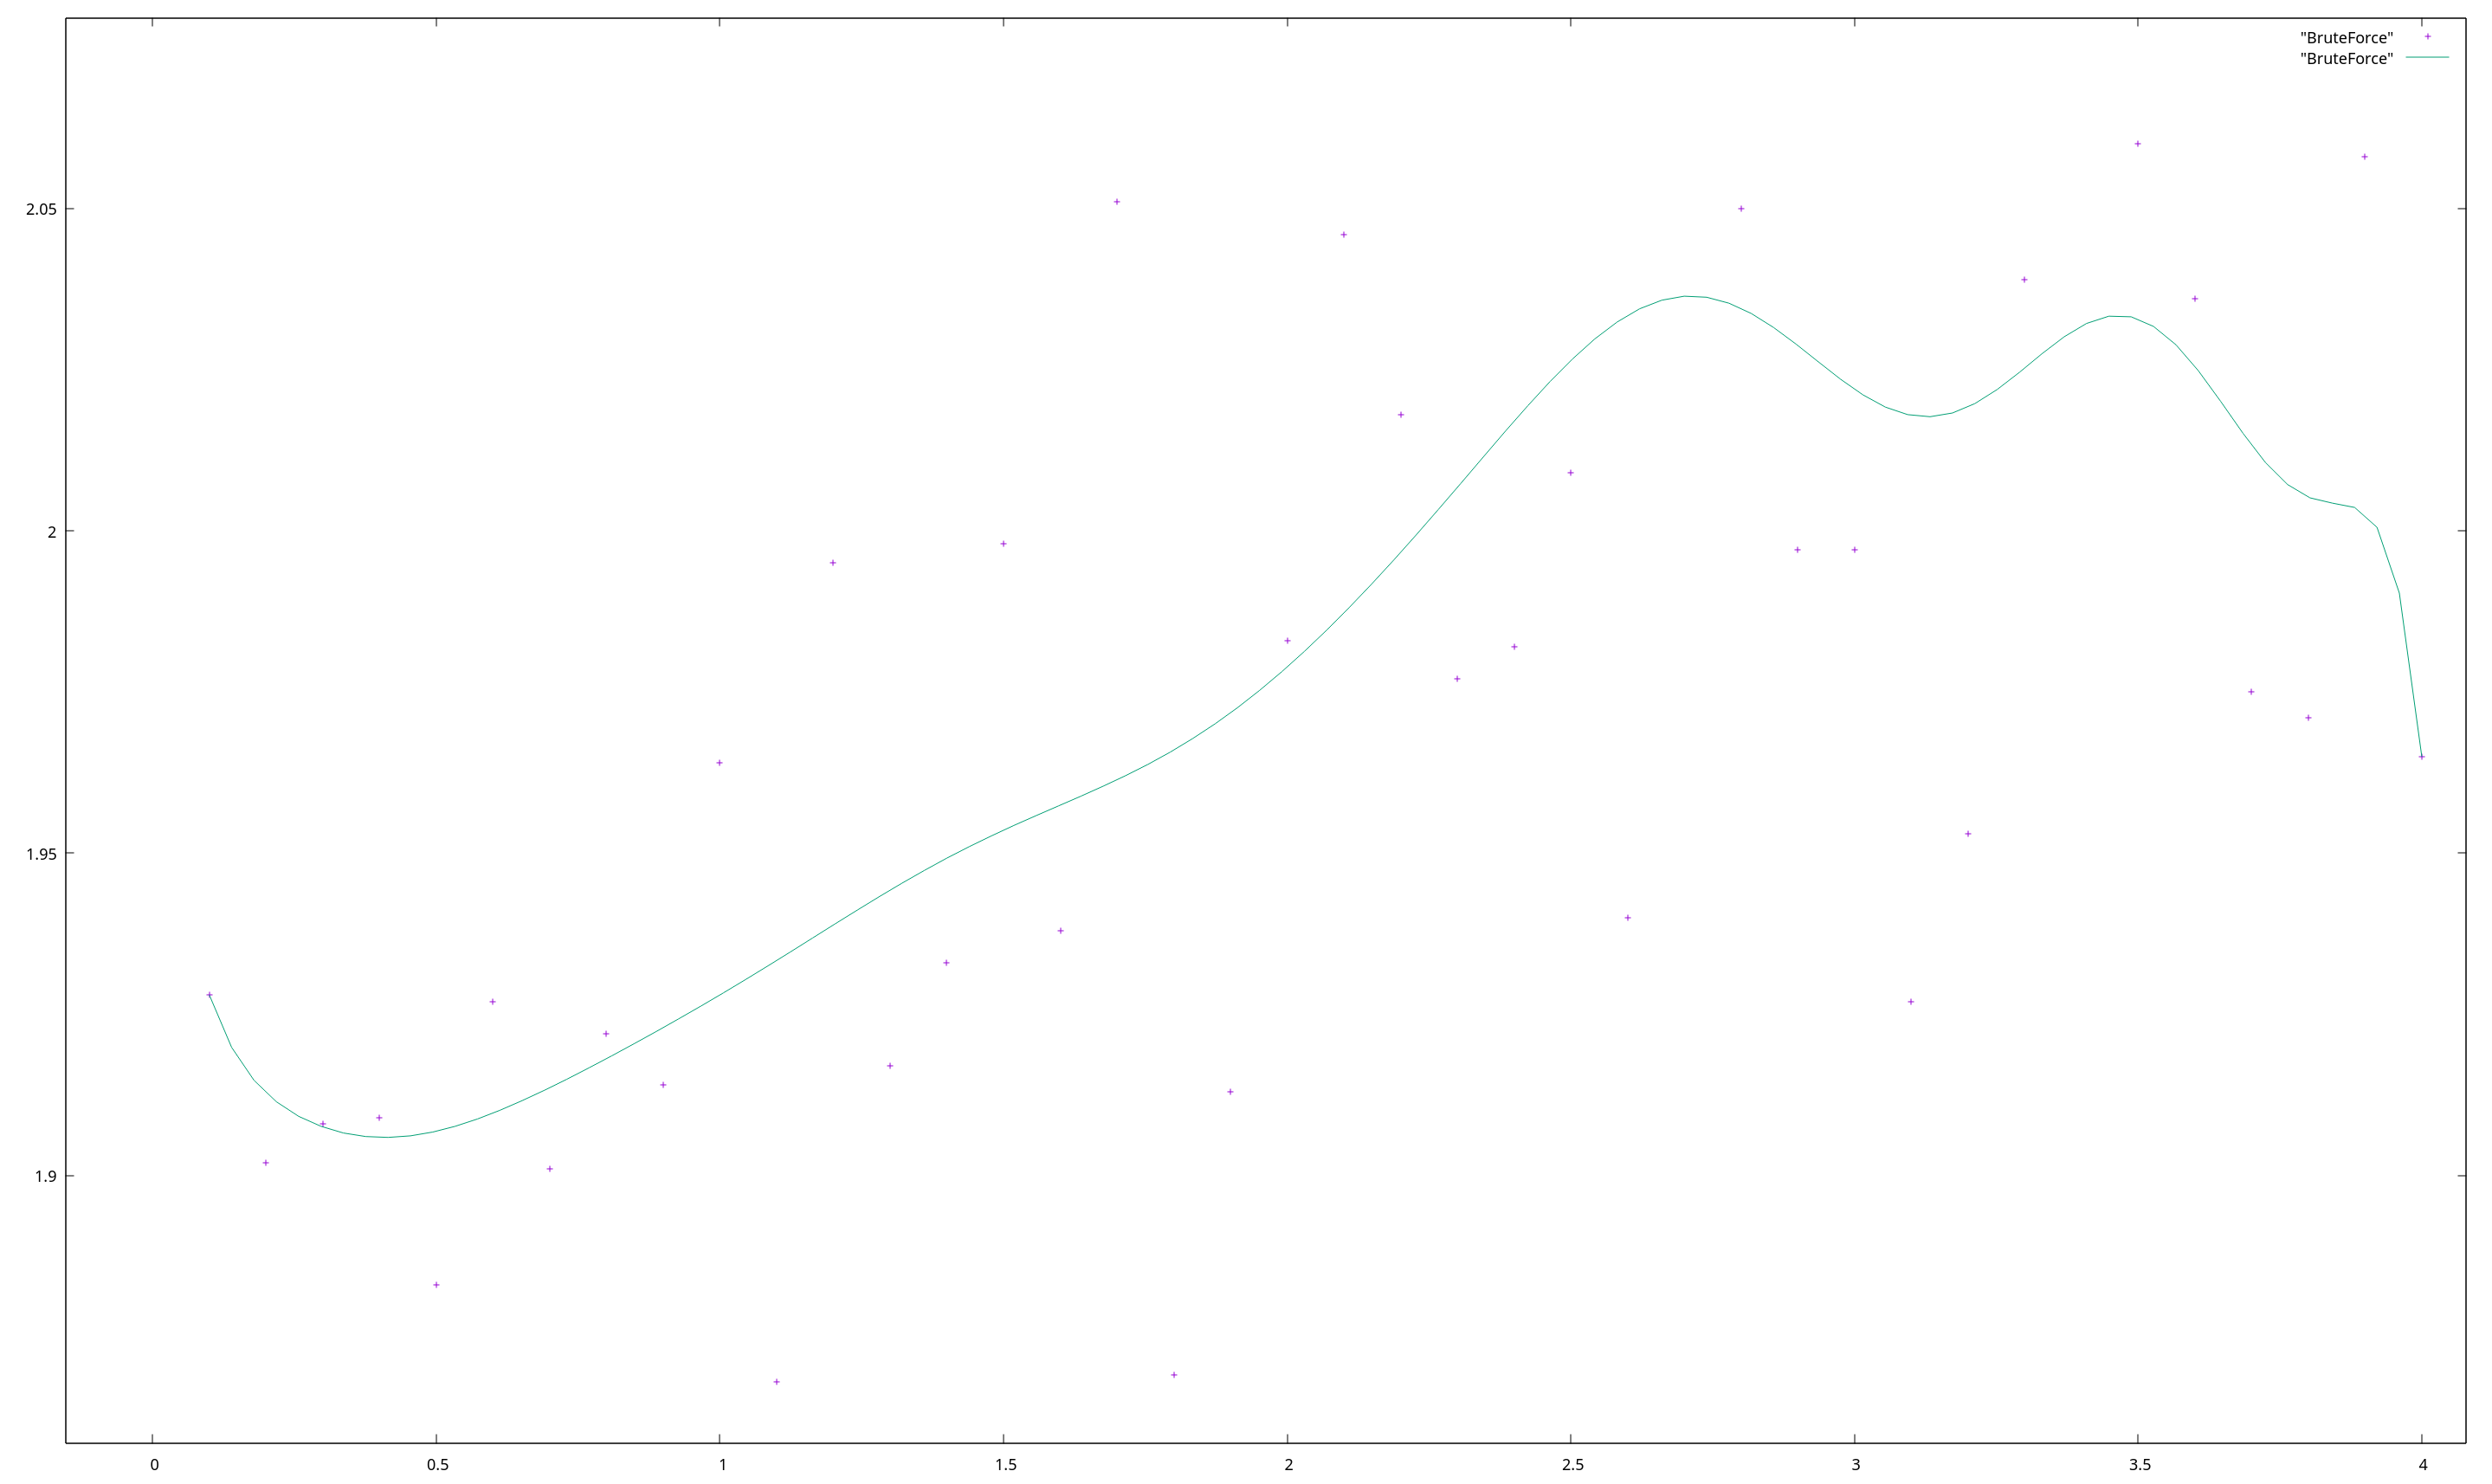
\includegraphics[width=\textwidth]{exp/small/BruteForce}
\caption{Vývoj času výpočtu hrubou silou (pro různý exponent, malé věci)}
\label{exp/small/BruteForce}
\end{center}
\end{figure}

Závislost pro metodu větví a hranic je v grafu \ref{exp/small/BranchNBound}. Je opět dosti náhodná. Ořezávání prostoru probíhá na základě výpočtů, které s granularitou nesouvisí. 

\begin{figure}[H]
\begin{center}
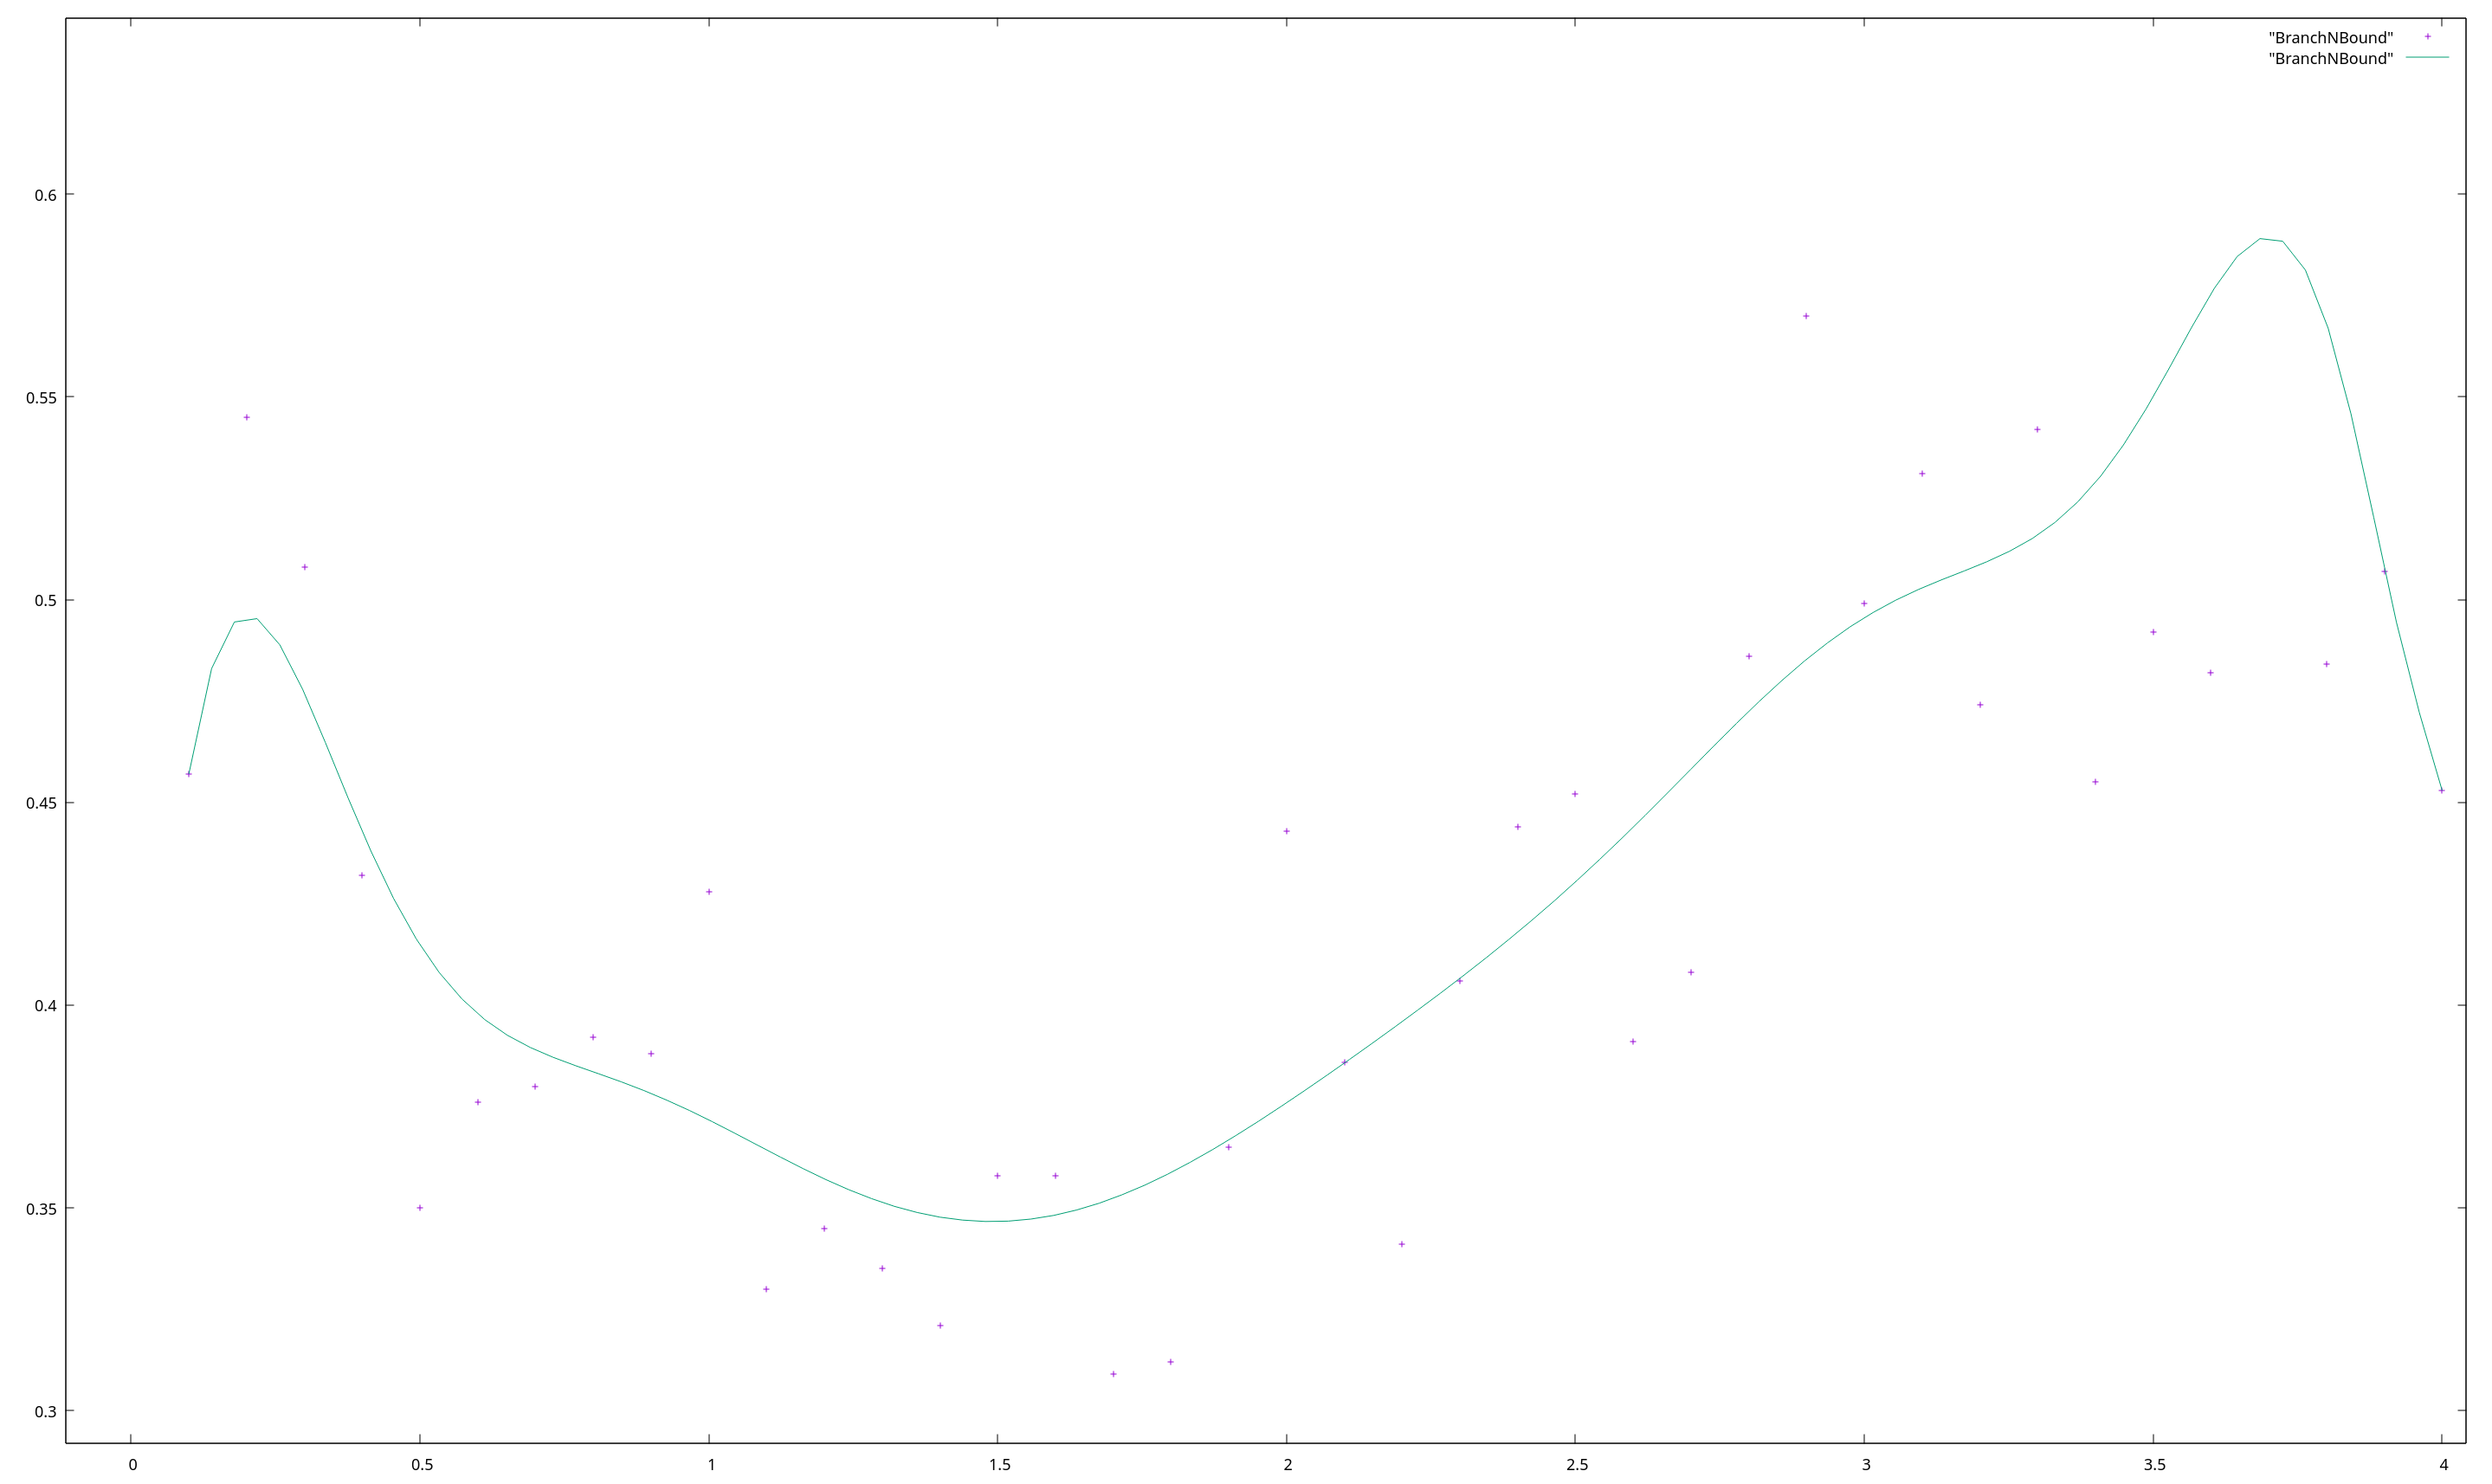
\includegraphics[width=\textwidth]{exp/small/BranchNBound}
\caption{Vývoj času výpočtu metodou větví a hranic (pro různý exponent, malé věci)}
\label{exp/small/BranchNBound}
\end{center}
\end{figure}

Závislost dekompozice podle ceny je vidět na obrázku \ref{exp/small/PriceDecomposition}. Opět není výrazná, naopak se zdá být náhodná. Tabulka dynamického programování má rozměry počtu instancí a součtu cen všech věcí a ani jedna z těchto hodnot nesouvisí s granularitou instance.

\begin{figure}[H]
\begin{center}
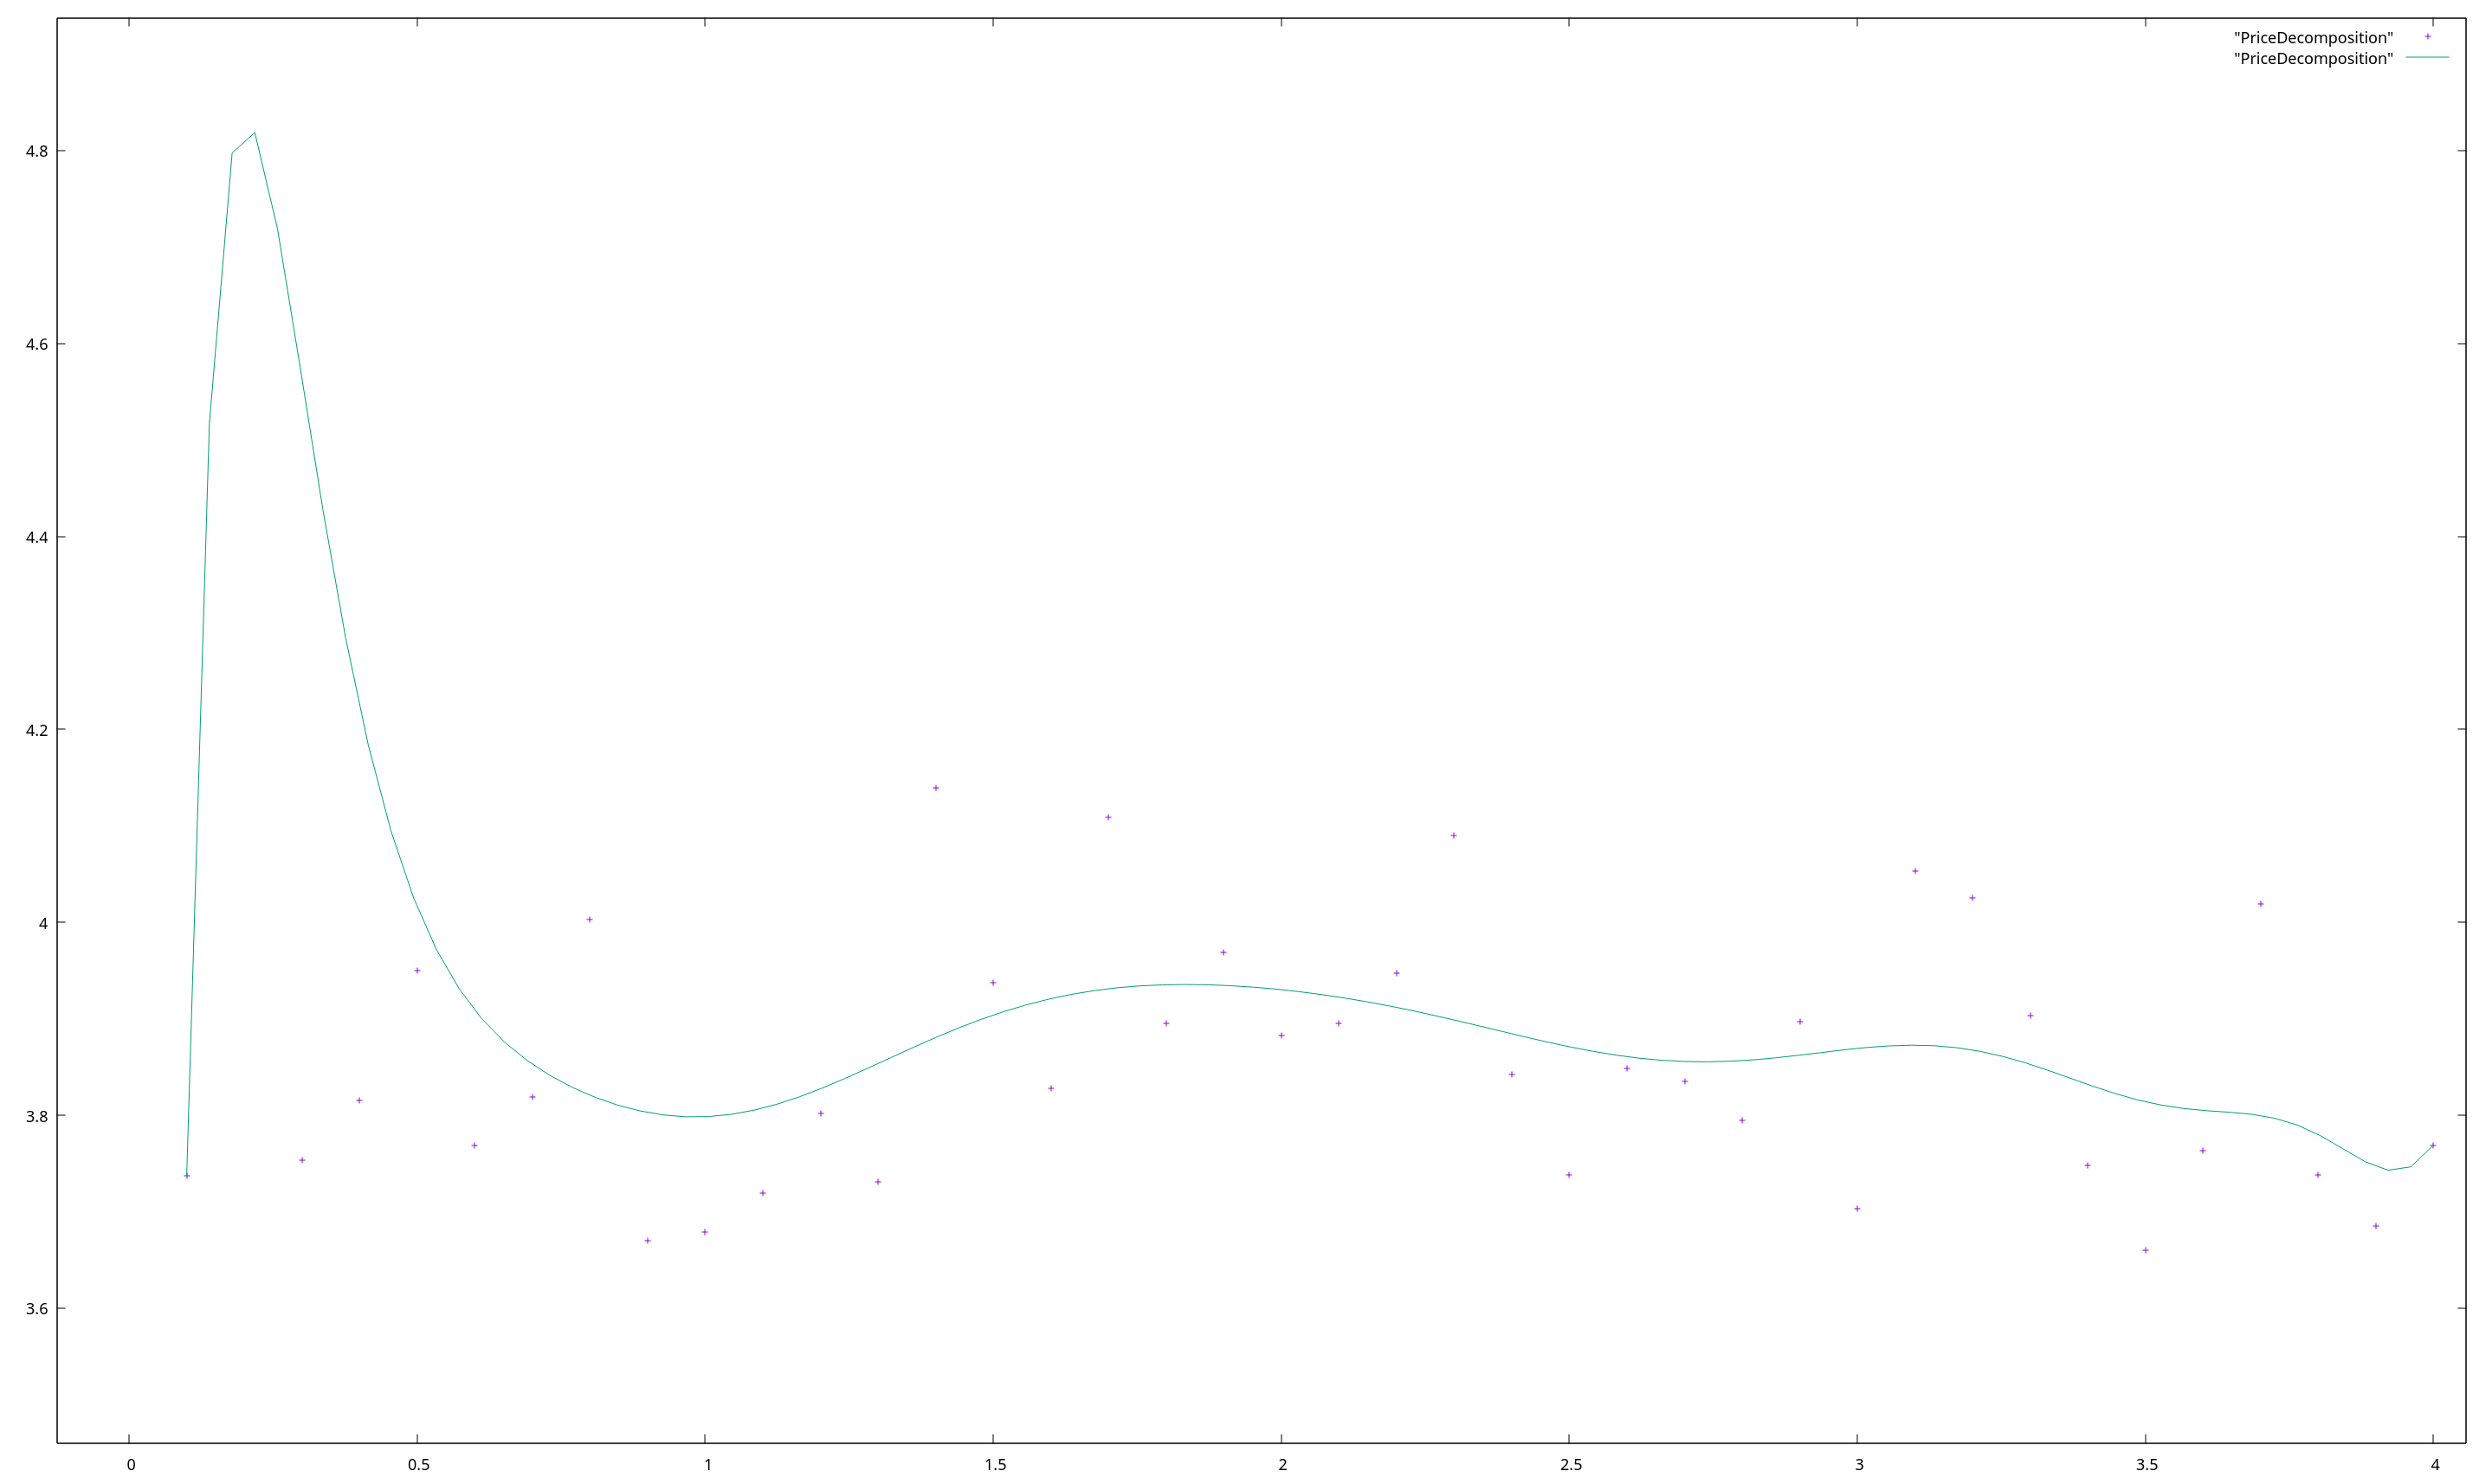
\includegraphics[width=\textwidth]{exp/small/PriceDecomposition}
\caption{Vývoj času výpočtu dekompozicí podle ceny (pro různý exponent, malé věci)}
\label{exp/small/PriceDecomposition}
\end{center}
\end{figure}

Ani heuristická metoda dle grafů \ref{exp/small/PriceToWeightRatio} a  \ref{exp/small/PriceToWeightRatio-relerrs} na granularitě nezávisí. 

\begin{figure}[H]
\begin{center}
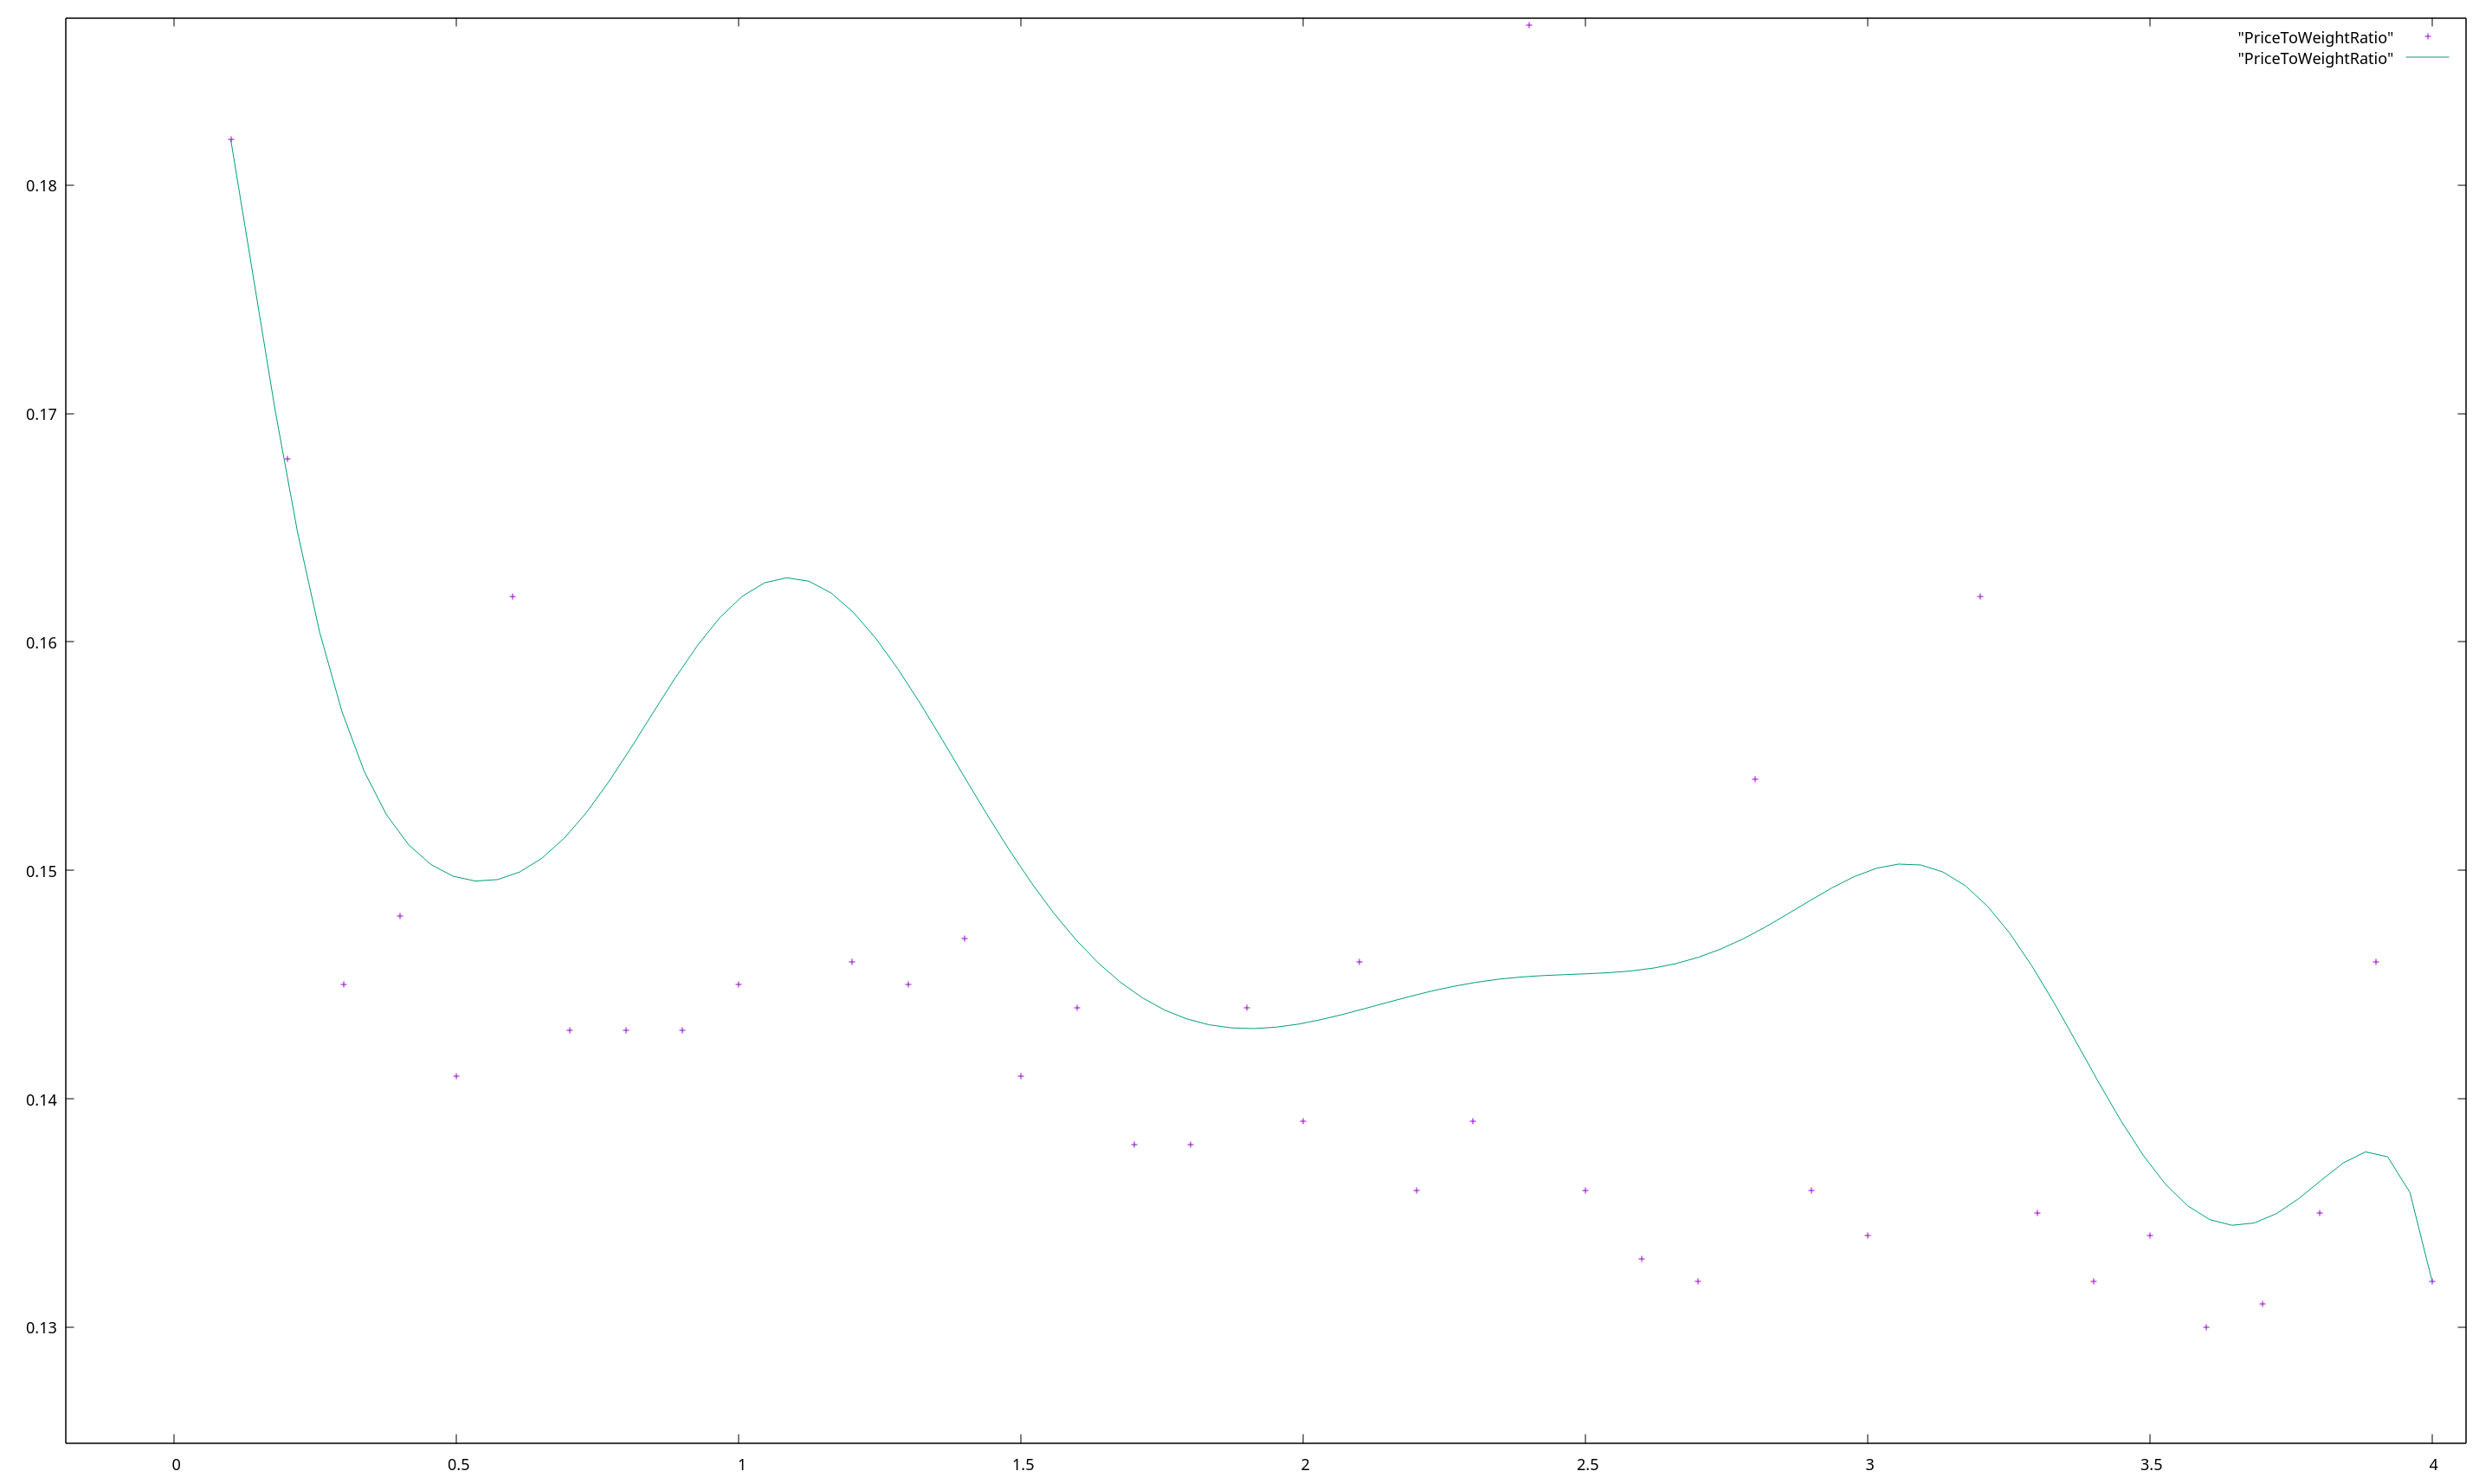
\includegraphics[width=\textwidth]{exp/small/PriceToWeightRatio}
\caption{Vývoj času výpočtu heuristikou (pro různý exponent, malé věci)}
\label{exp/small/PriceToWeightRatio}
\end{center}
\end{figure}

\begin{figure}[H]
\begin{center}
\includegraphics[width=\textwidth]{exp/small/PriceToWeightRatio-relerrs}
\caption{Vývoj relativní chyby výpočtu heuristikou (pro různý exponent, malé věci)}
\label{exp/small/PriceToWeightRatio-relerrs}
\end{center}
\end{figure}

Srovnání těchto metod z hlediska výpočetního času je vidět v grafu \ref{exp/small/allExecTimes}. Z grafu je patrné, že žádná z metod není závislá na exponentu určujícím, jak velký důraz je kladen na výběr lehkých věcí.

\begin{figure}[H]
\begin{center}
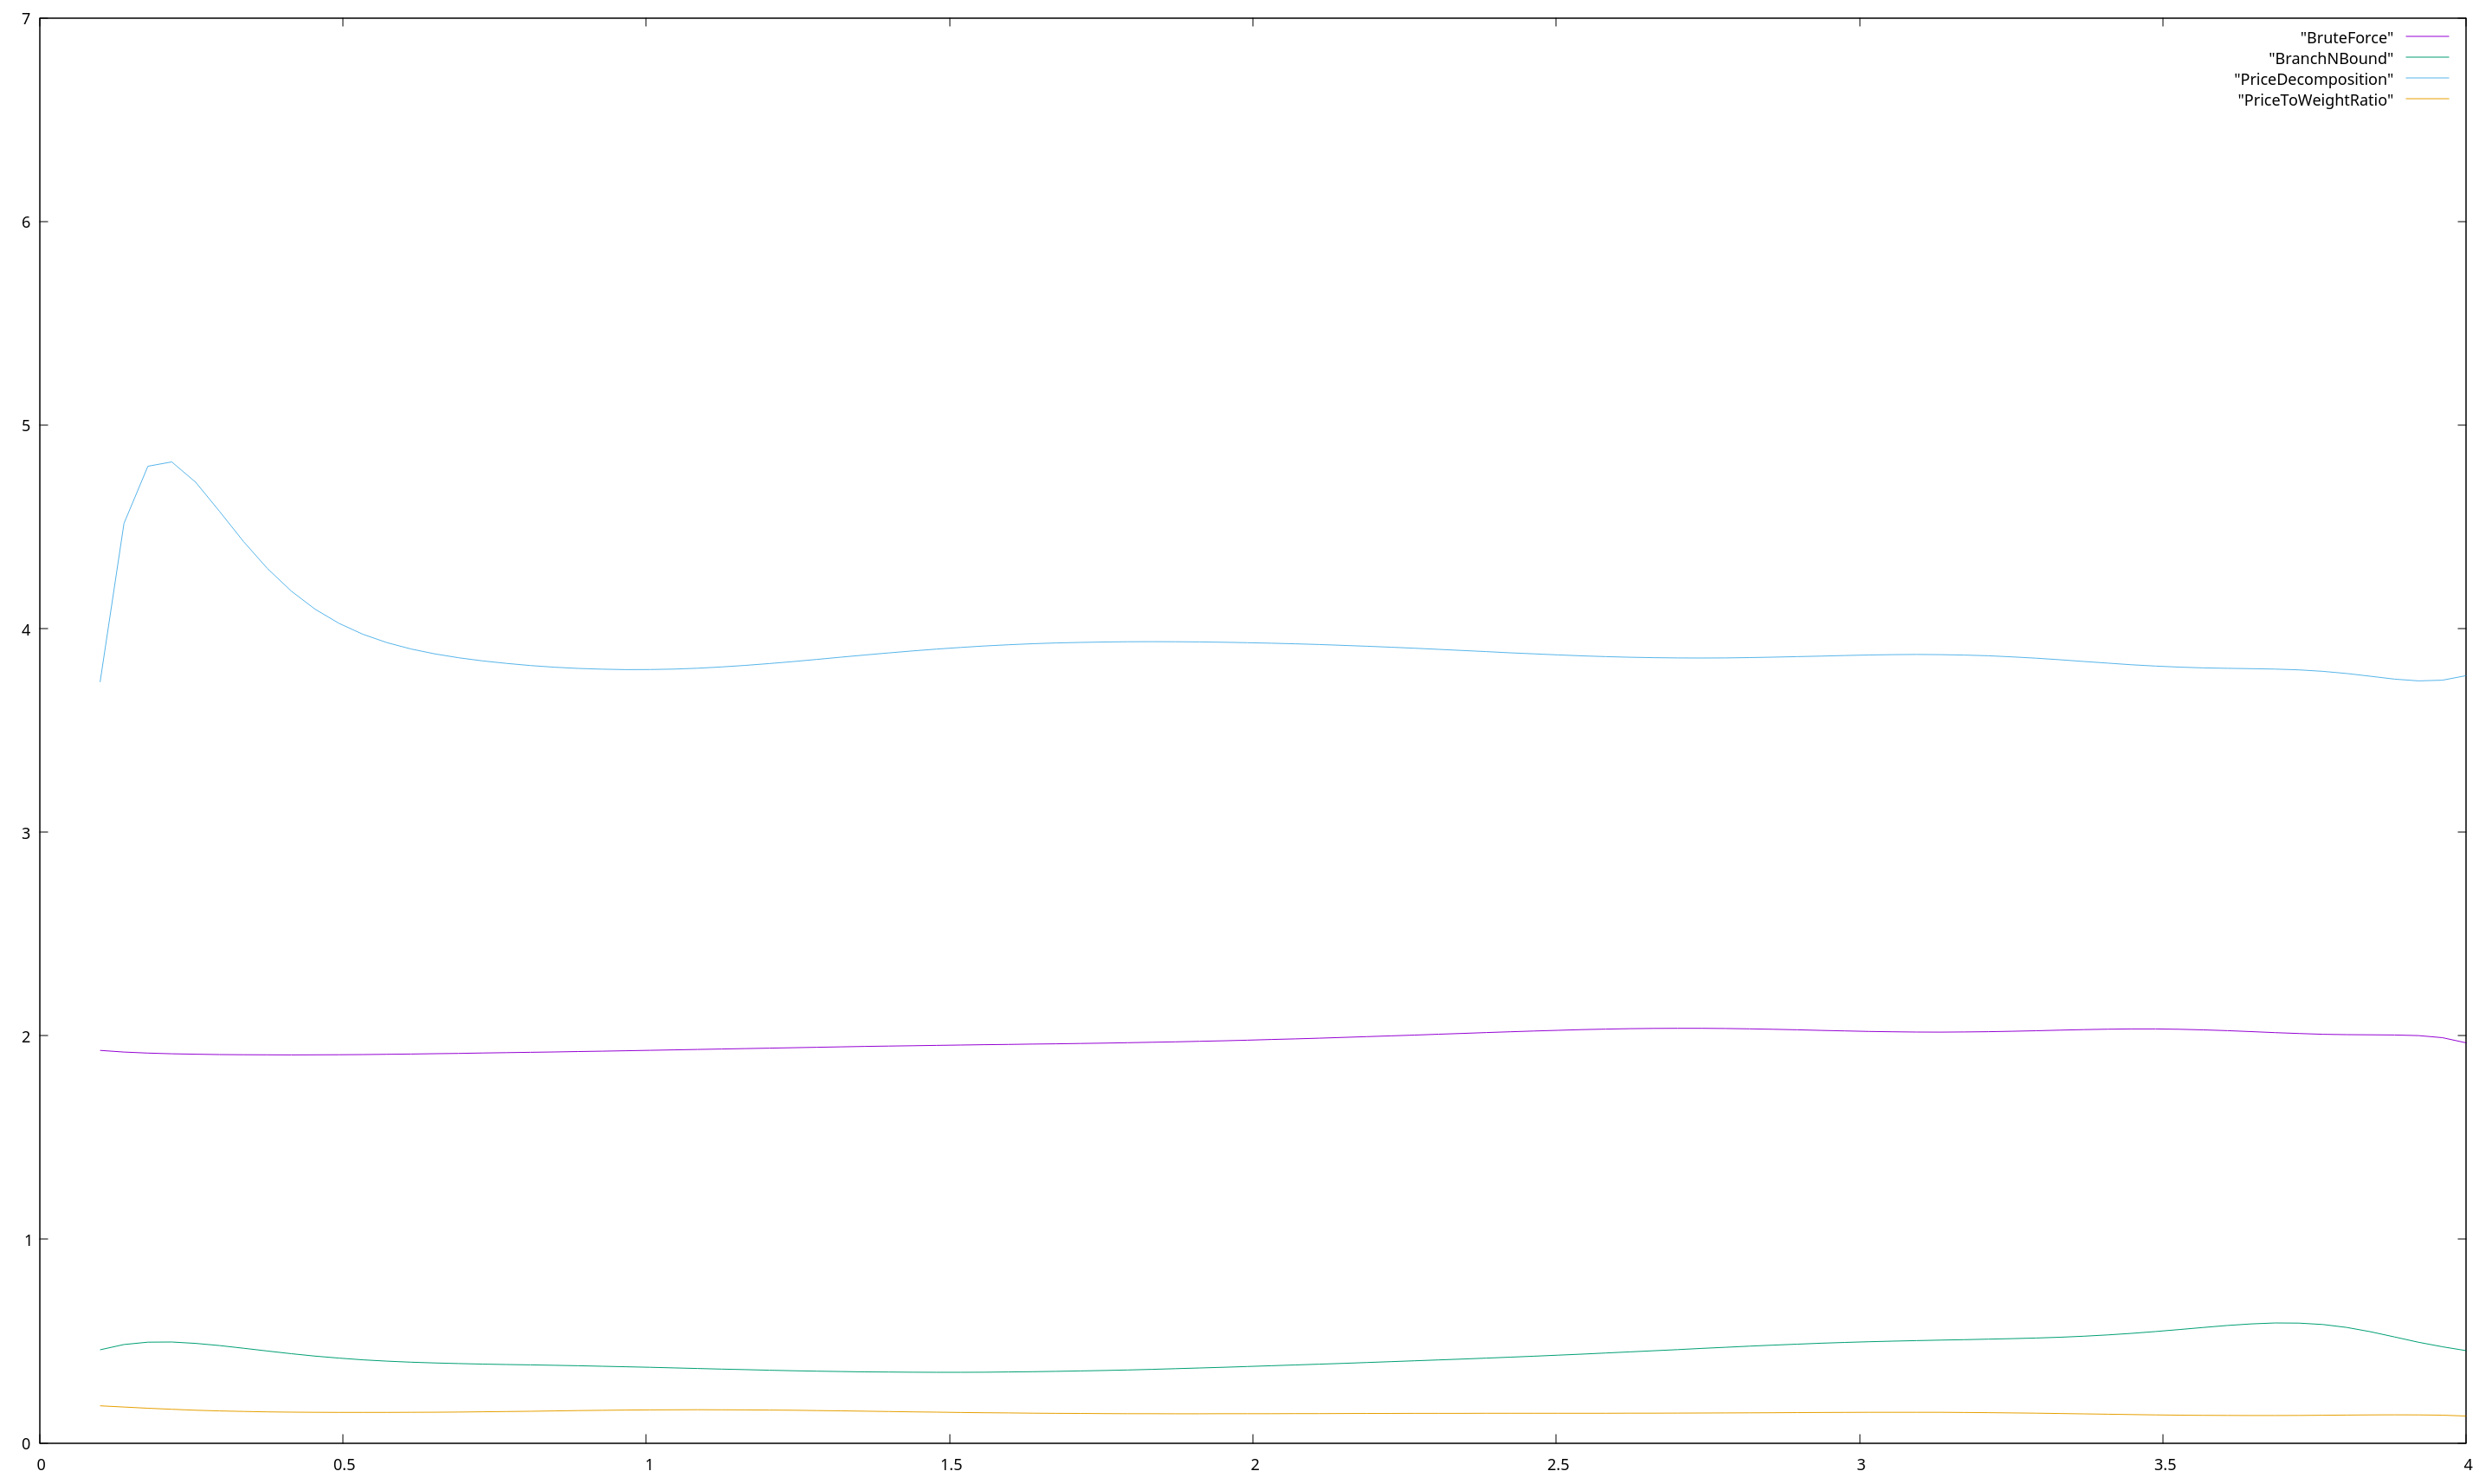
\includegraphics[width=\textwidth]{exp/small/allExecTimes}
\caption{Srovnání závislosti metod na exponentu určujícím převahu malých věcí}
\label{exp/small/allExecTimes}
\end{center}
\end{figure}







\subsection{Převaha velkých věcí}

Stejně tak lze měnit exponent výpočtu použitého při výběru věcí tak, aby byly spíše těžší. Exponent pak má ten význam, že čím je větší, tím větší věci budou vybírány. Hraje roli exponentu $k$ ve vzorci $1/(w_{max}-w)^k$ pro pravděpodobnost zahrnutí předmětu o váze $w$, čili čím větší je exponent, tím se pro stejnou váhu pravděpodobnost snižuje, musíme vzít těžší.

Tento exponent jsem opět měnil v rozmezí 0.1 a 4.0 se skokem 0.1 s účelem získat 40 měření, každé provedené na padesáti vygenerovaných instancí daných vlastností. 

Řešení hrubou silou je vyobrazeno v grafu \ref{exp/big/BruteForce}. Graf je docela přesně lineární, závislost zde není. Metoda hrubé síly prochází celý stavový prostor a podoba vah nemá na průchod vliv.

\begin{figure}[H]
\begin{center}
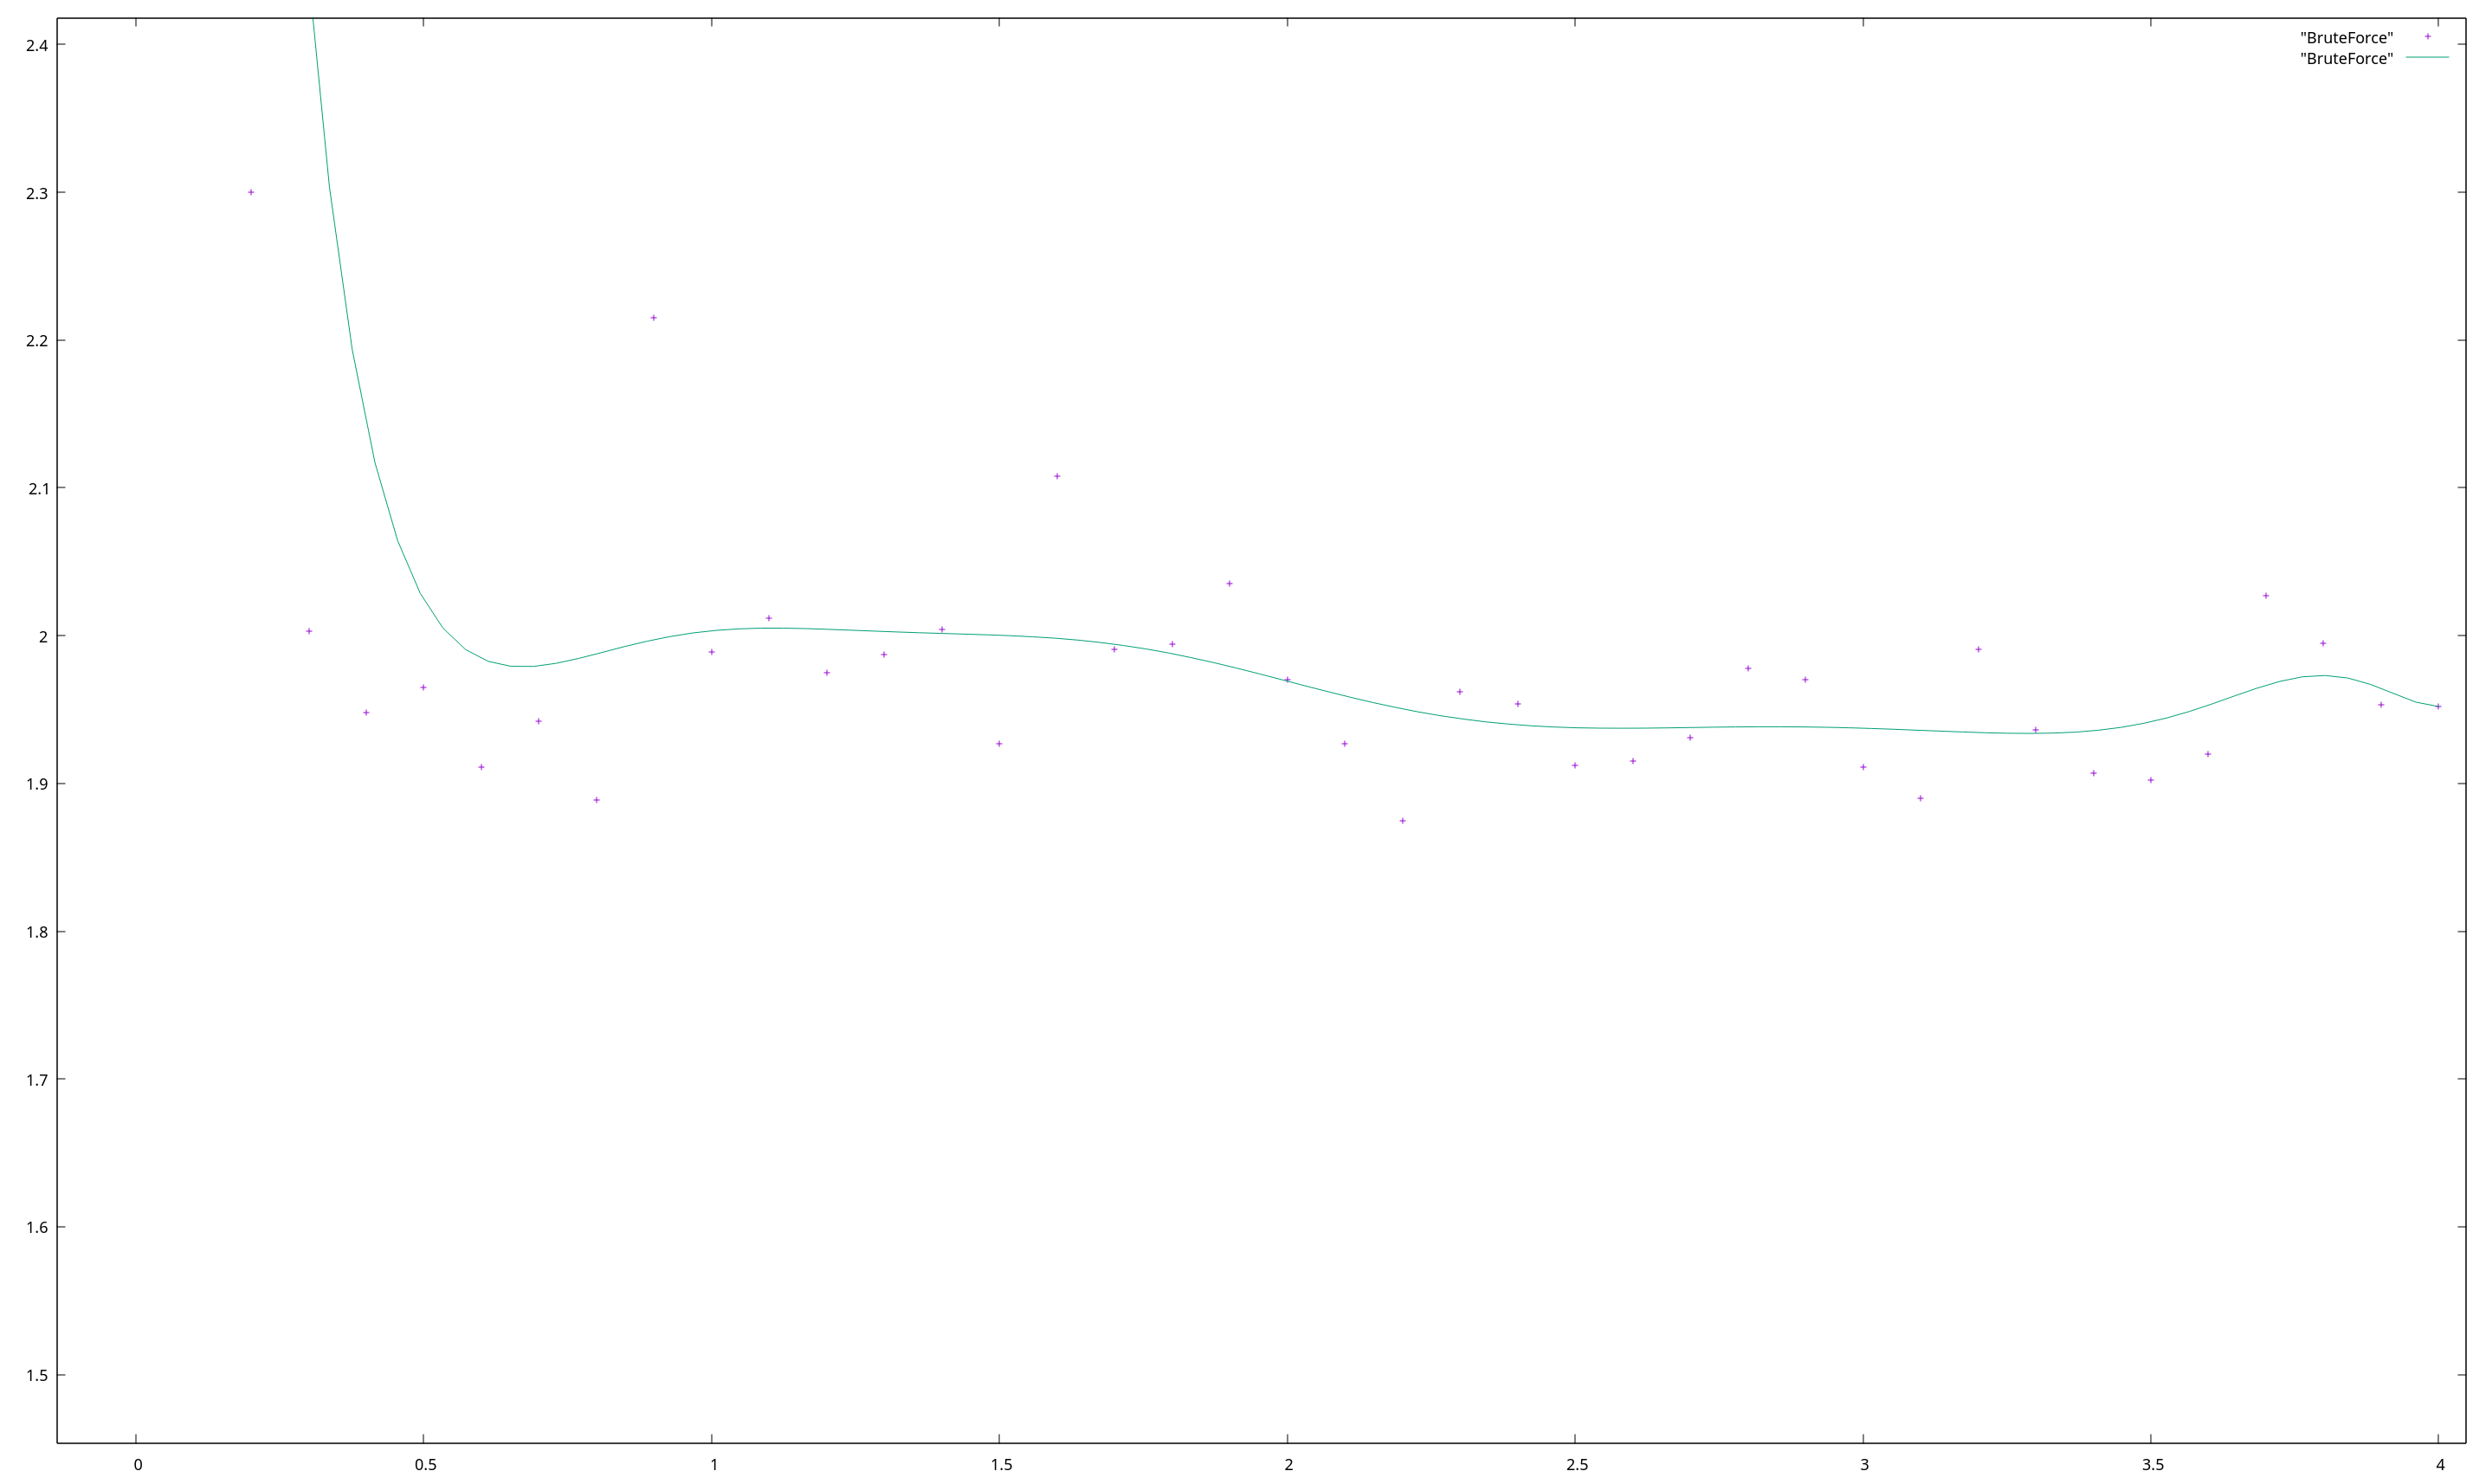
\includegraphics[width=\textwidth]{exp/big/BruteForce}
\caption{Vývoj času výpočtu hrubou silou (pro různý exponent, velké věci)}
\label{exp/big/BruteForce}
\end{center}
\end{figure}

Graf \ref{exp/big/BranchNBound} zobrazuje závislost v případě metody větví a hranic. Zde se zdá, že jistá závislost je, graf mírně stoupá pro silnější převahu větších věcí. Vzhledem k tomu, že se ale metoda rozhoduje ořezávat stavový prostor čistě na základě možného zlepšení ceny, přisuzuji toto chování grafu náhodě.

\begin{figure}[H]
\begin{center}
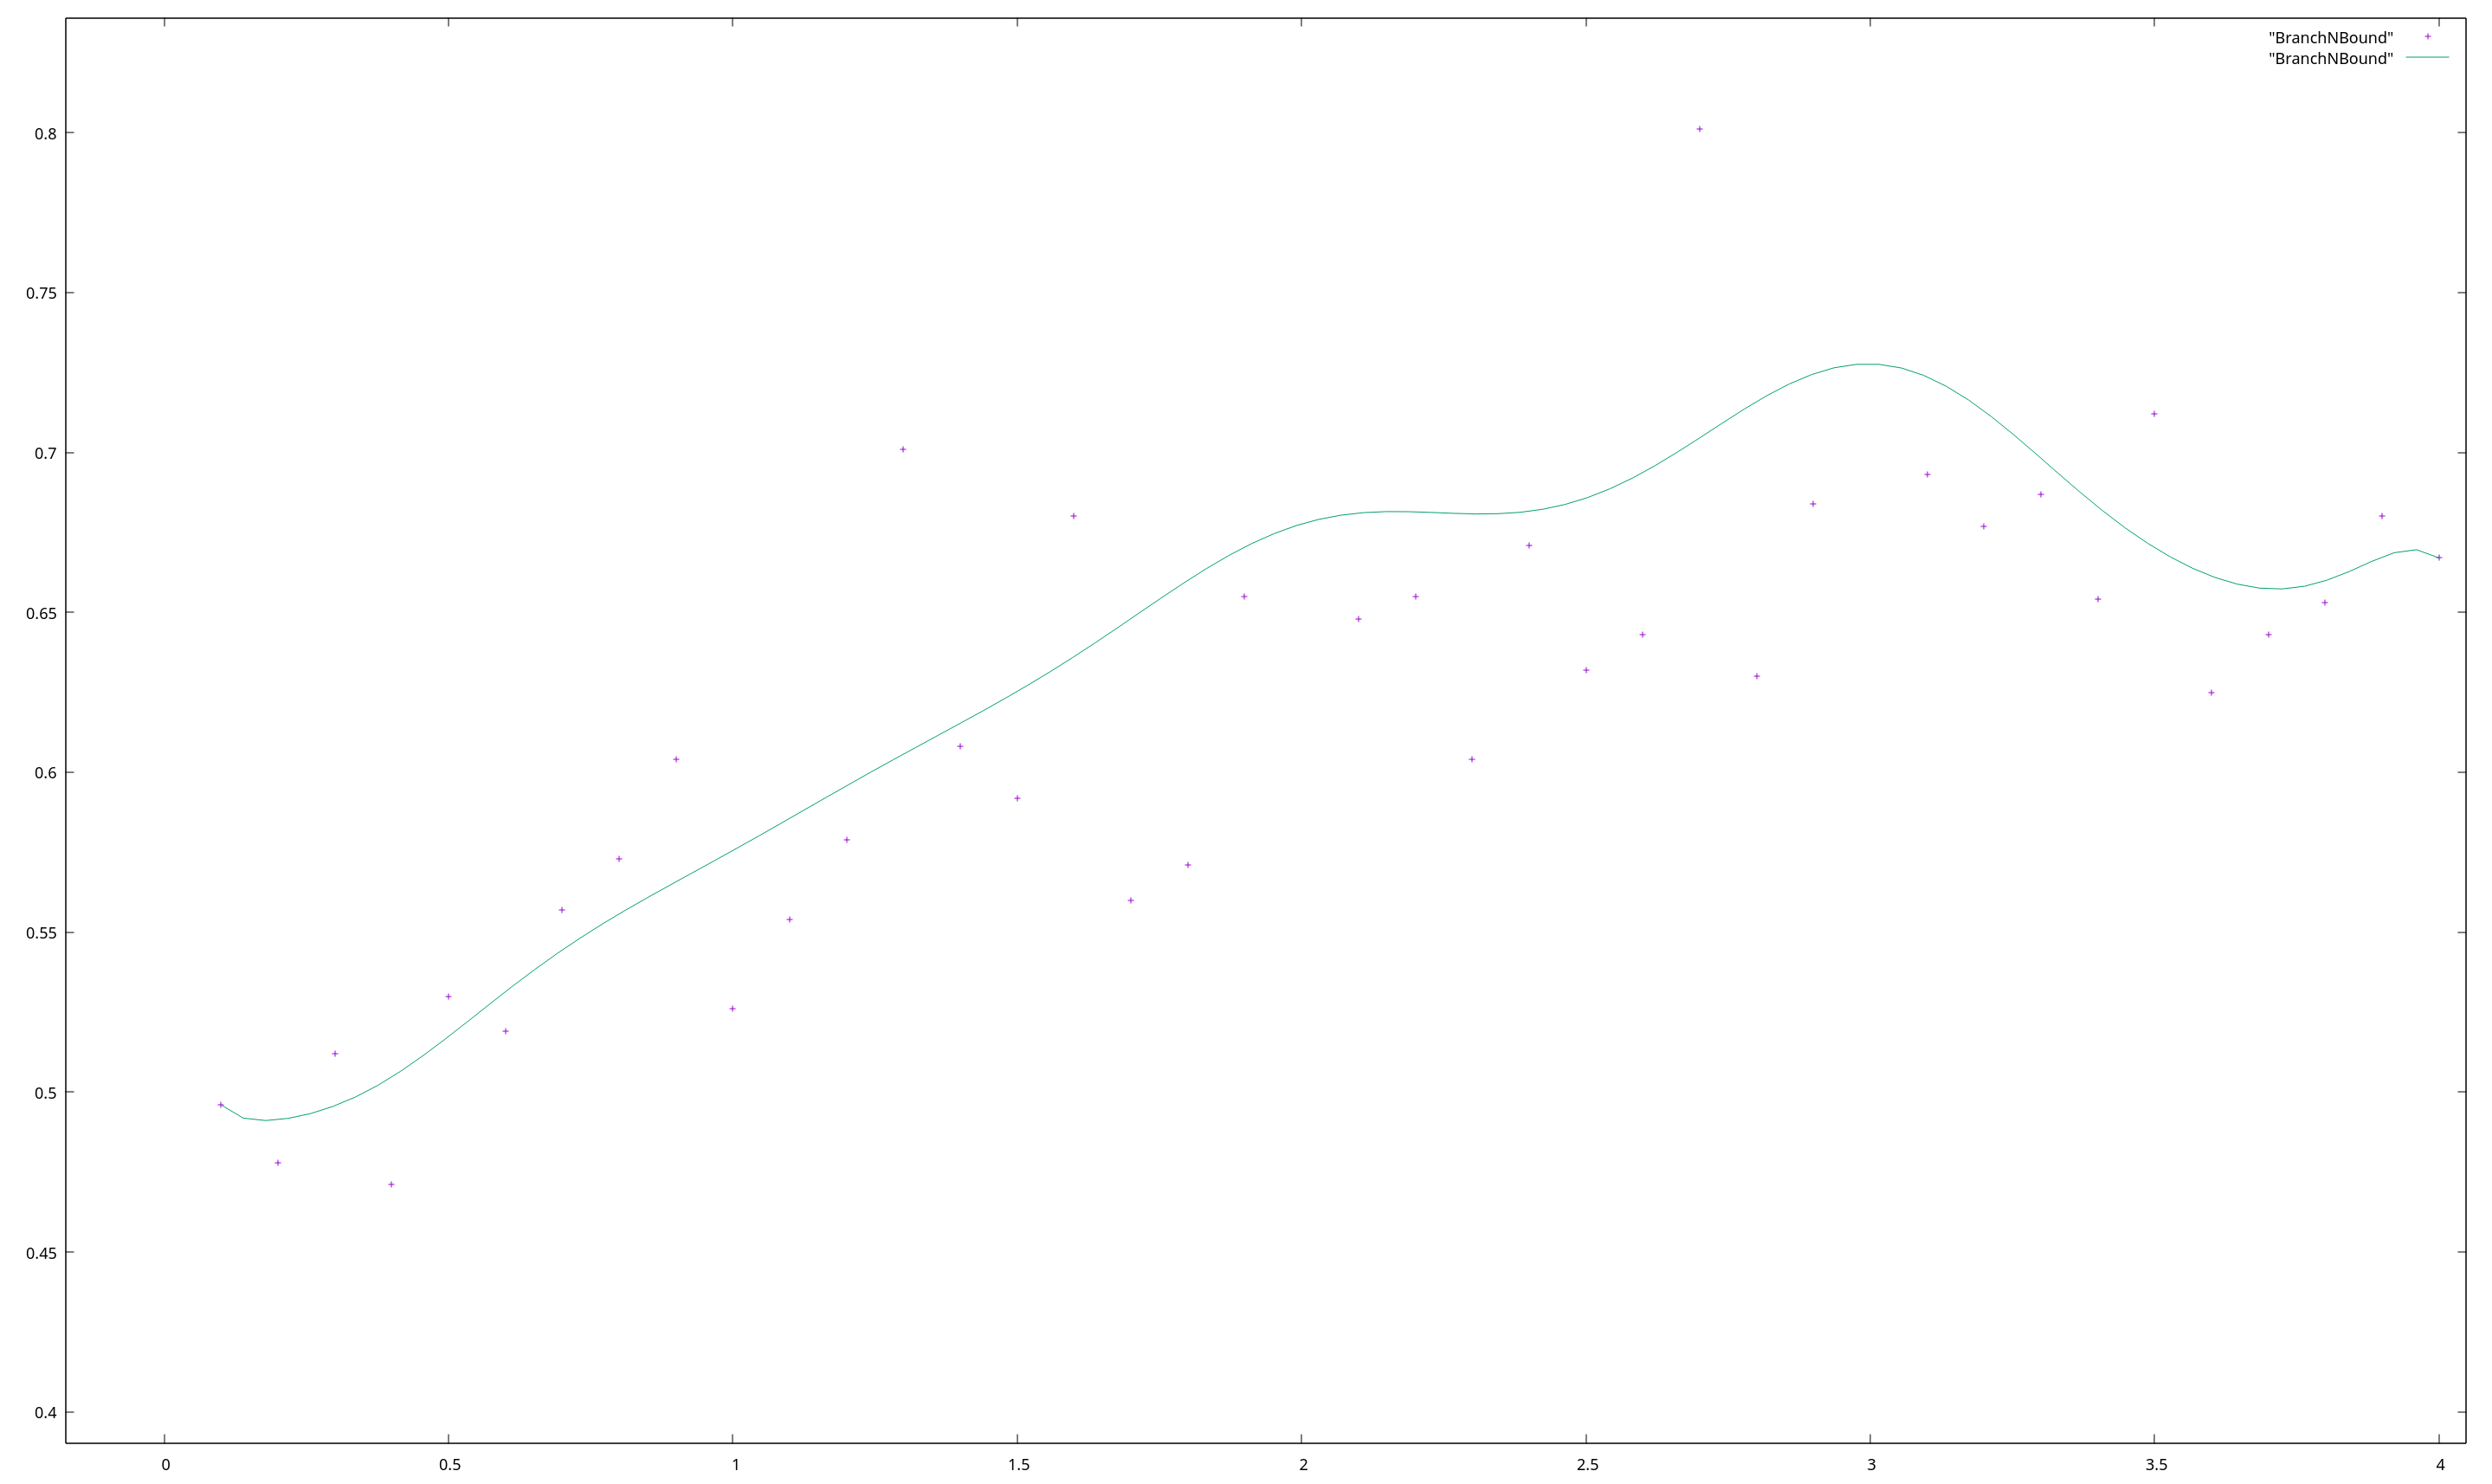
\includegraphics[width=\textwidth]{exp/big/BranchNBound}
\caption{Vývoj času výpočtu metodou větví a hranic (pro různý exponent, velké věci)}
\label{exp/big/BranchNBound}
\end{center}
\end{figure}

Dekompozice podle ceny podle grafu \ref{exp/big/PriceDecomposition} na různé převaze velkých věcí závislá není. Graf je více méně lineární. Tabulka dynamického programování není závislá na hodnotách vah, které do ní píšeme.

\begin{figure}[H]
\begin{center}
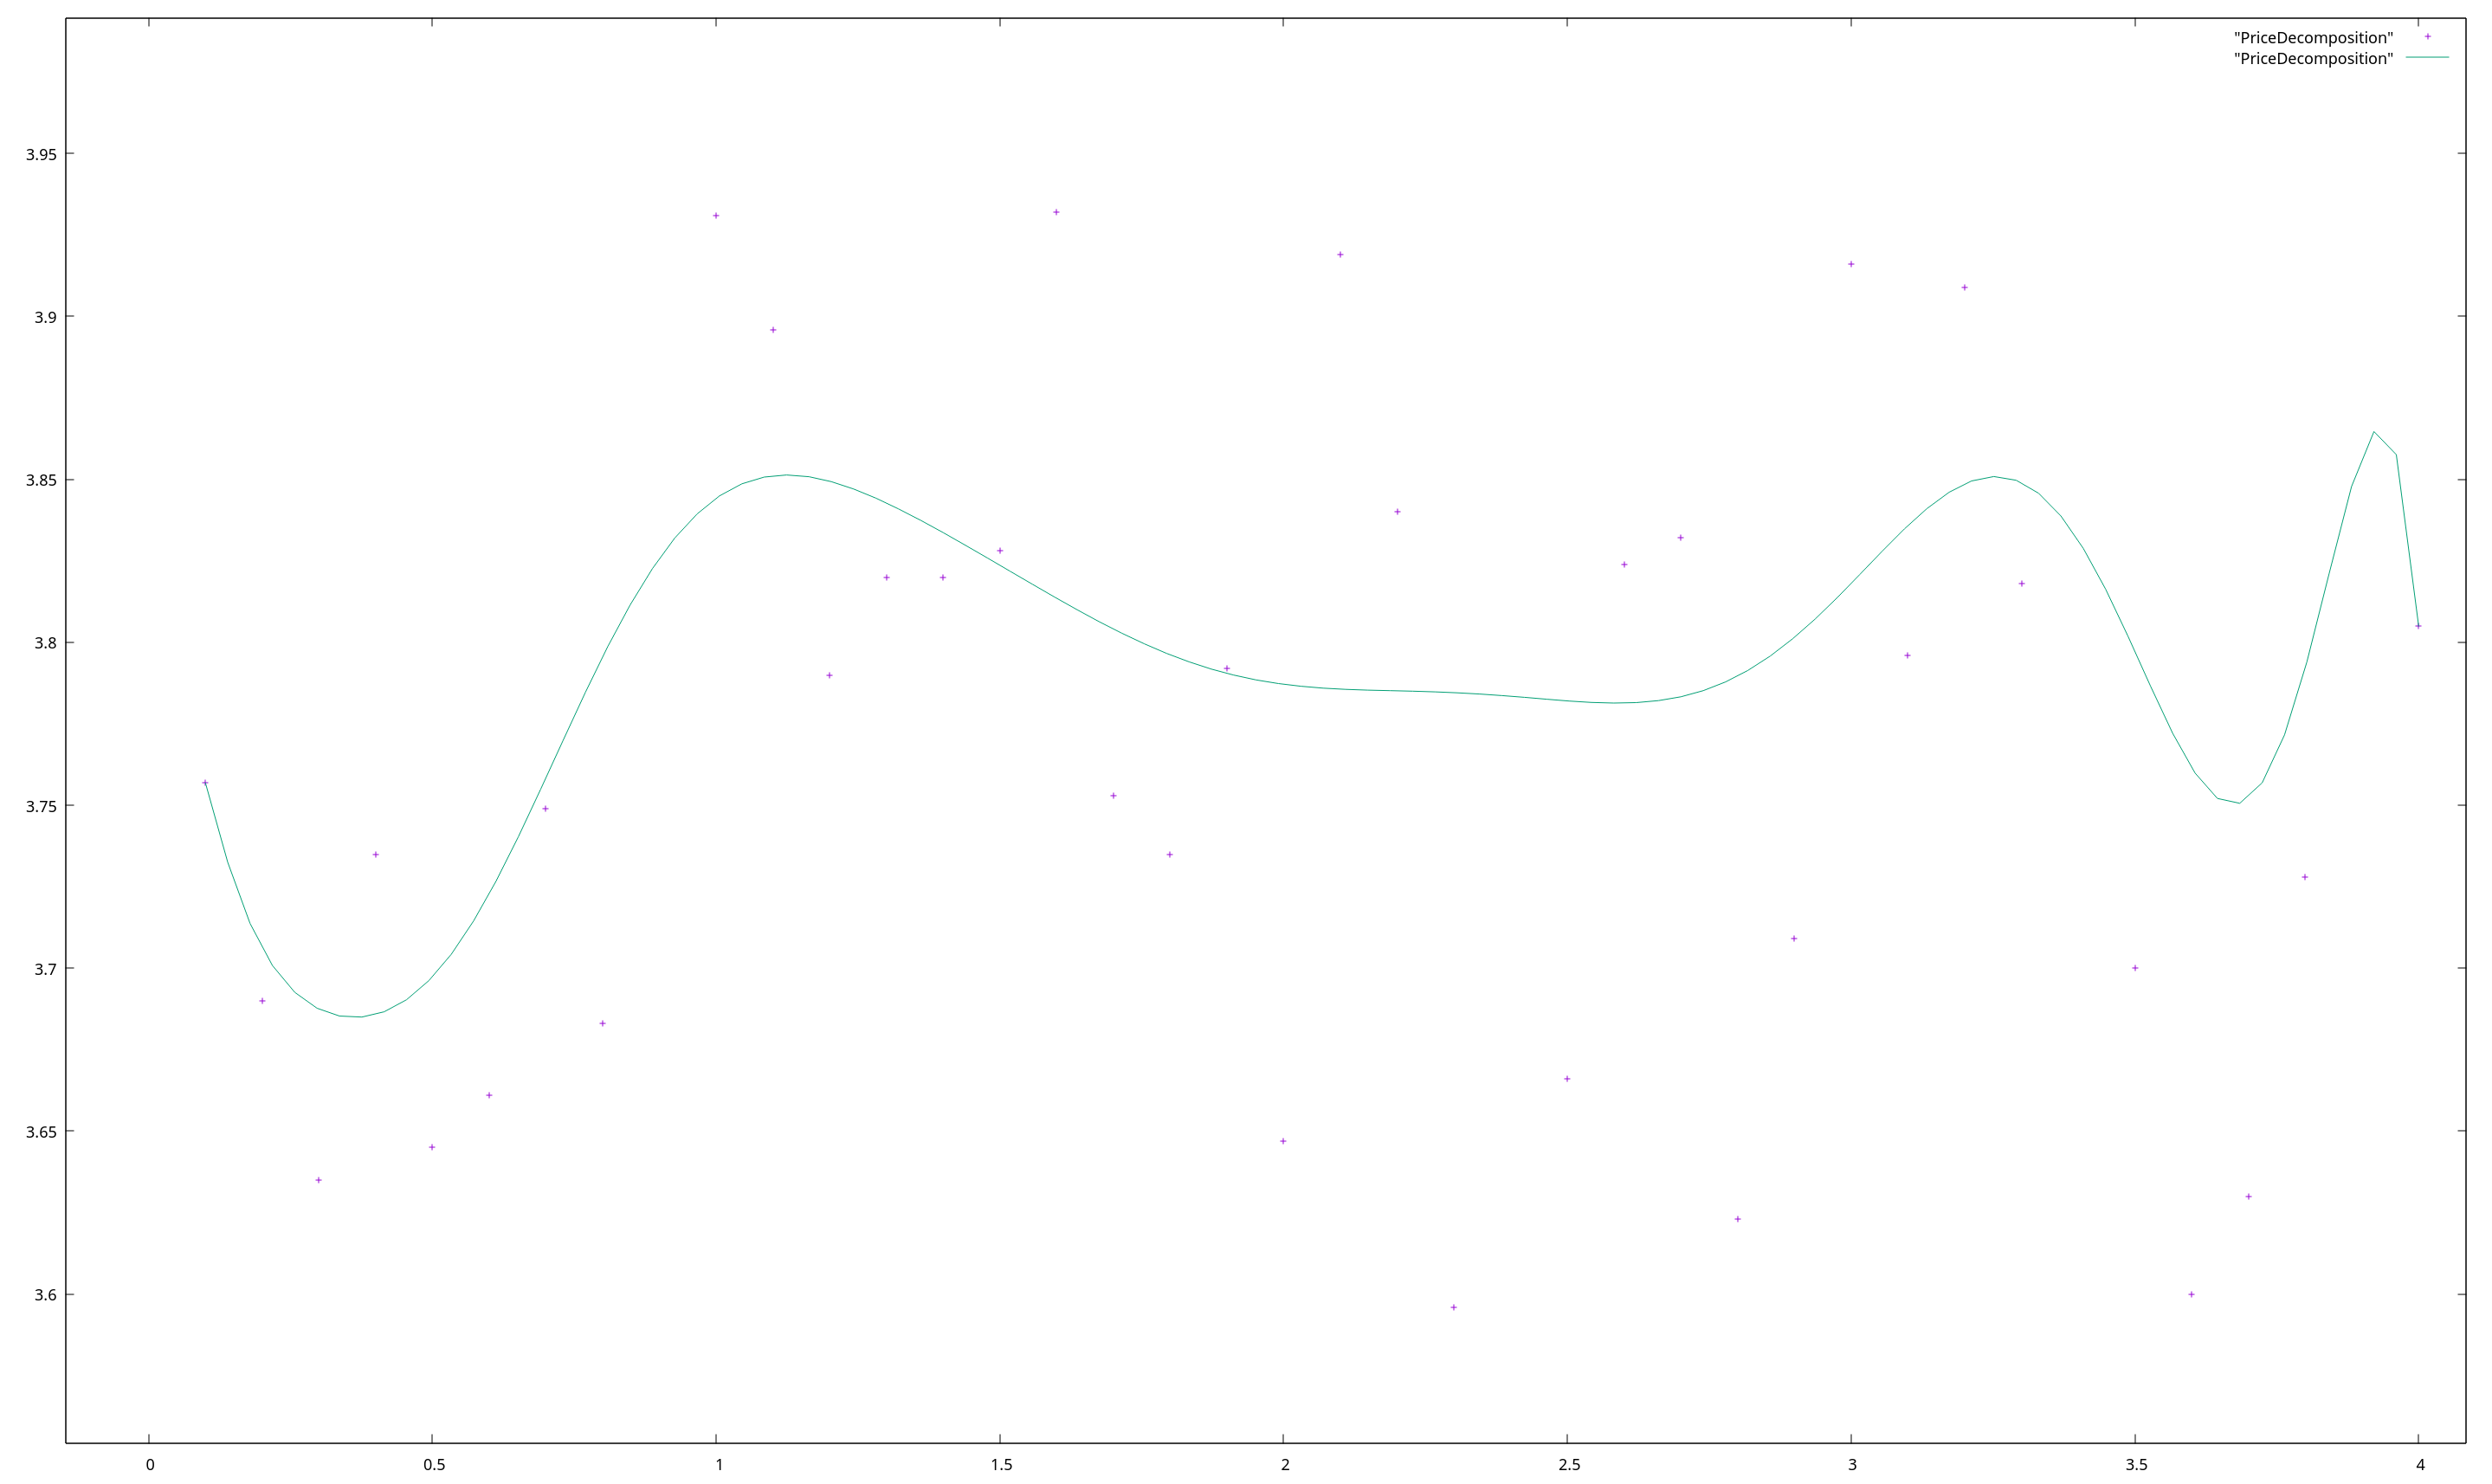
\includegraphics[width=\textwidth]{exp/big/PriceDecomposition}
\caption{Vývoj času výpočtu dekompozicí podle ceny (pro různý exponent, velké věci)}
\label{exp/big/PriceDecomposition}
\end{center}
\end{figure}

Ani heuristika není závislá na převaze velkých věcí, viz \ref{exp/big/PriceToWeightRatio}. Poměr, na základě nějž se heuristika rozhoduje, kterou věc vybere jako další není ovlivněn tím, zda jsou věci lehké nebo těžké.

\begin{figure}[H]
\begin{center}
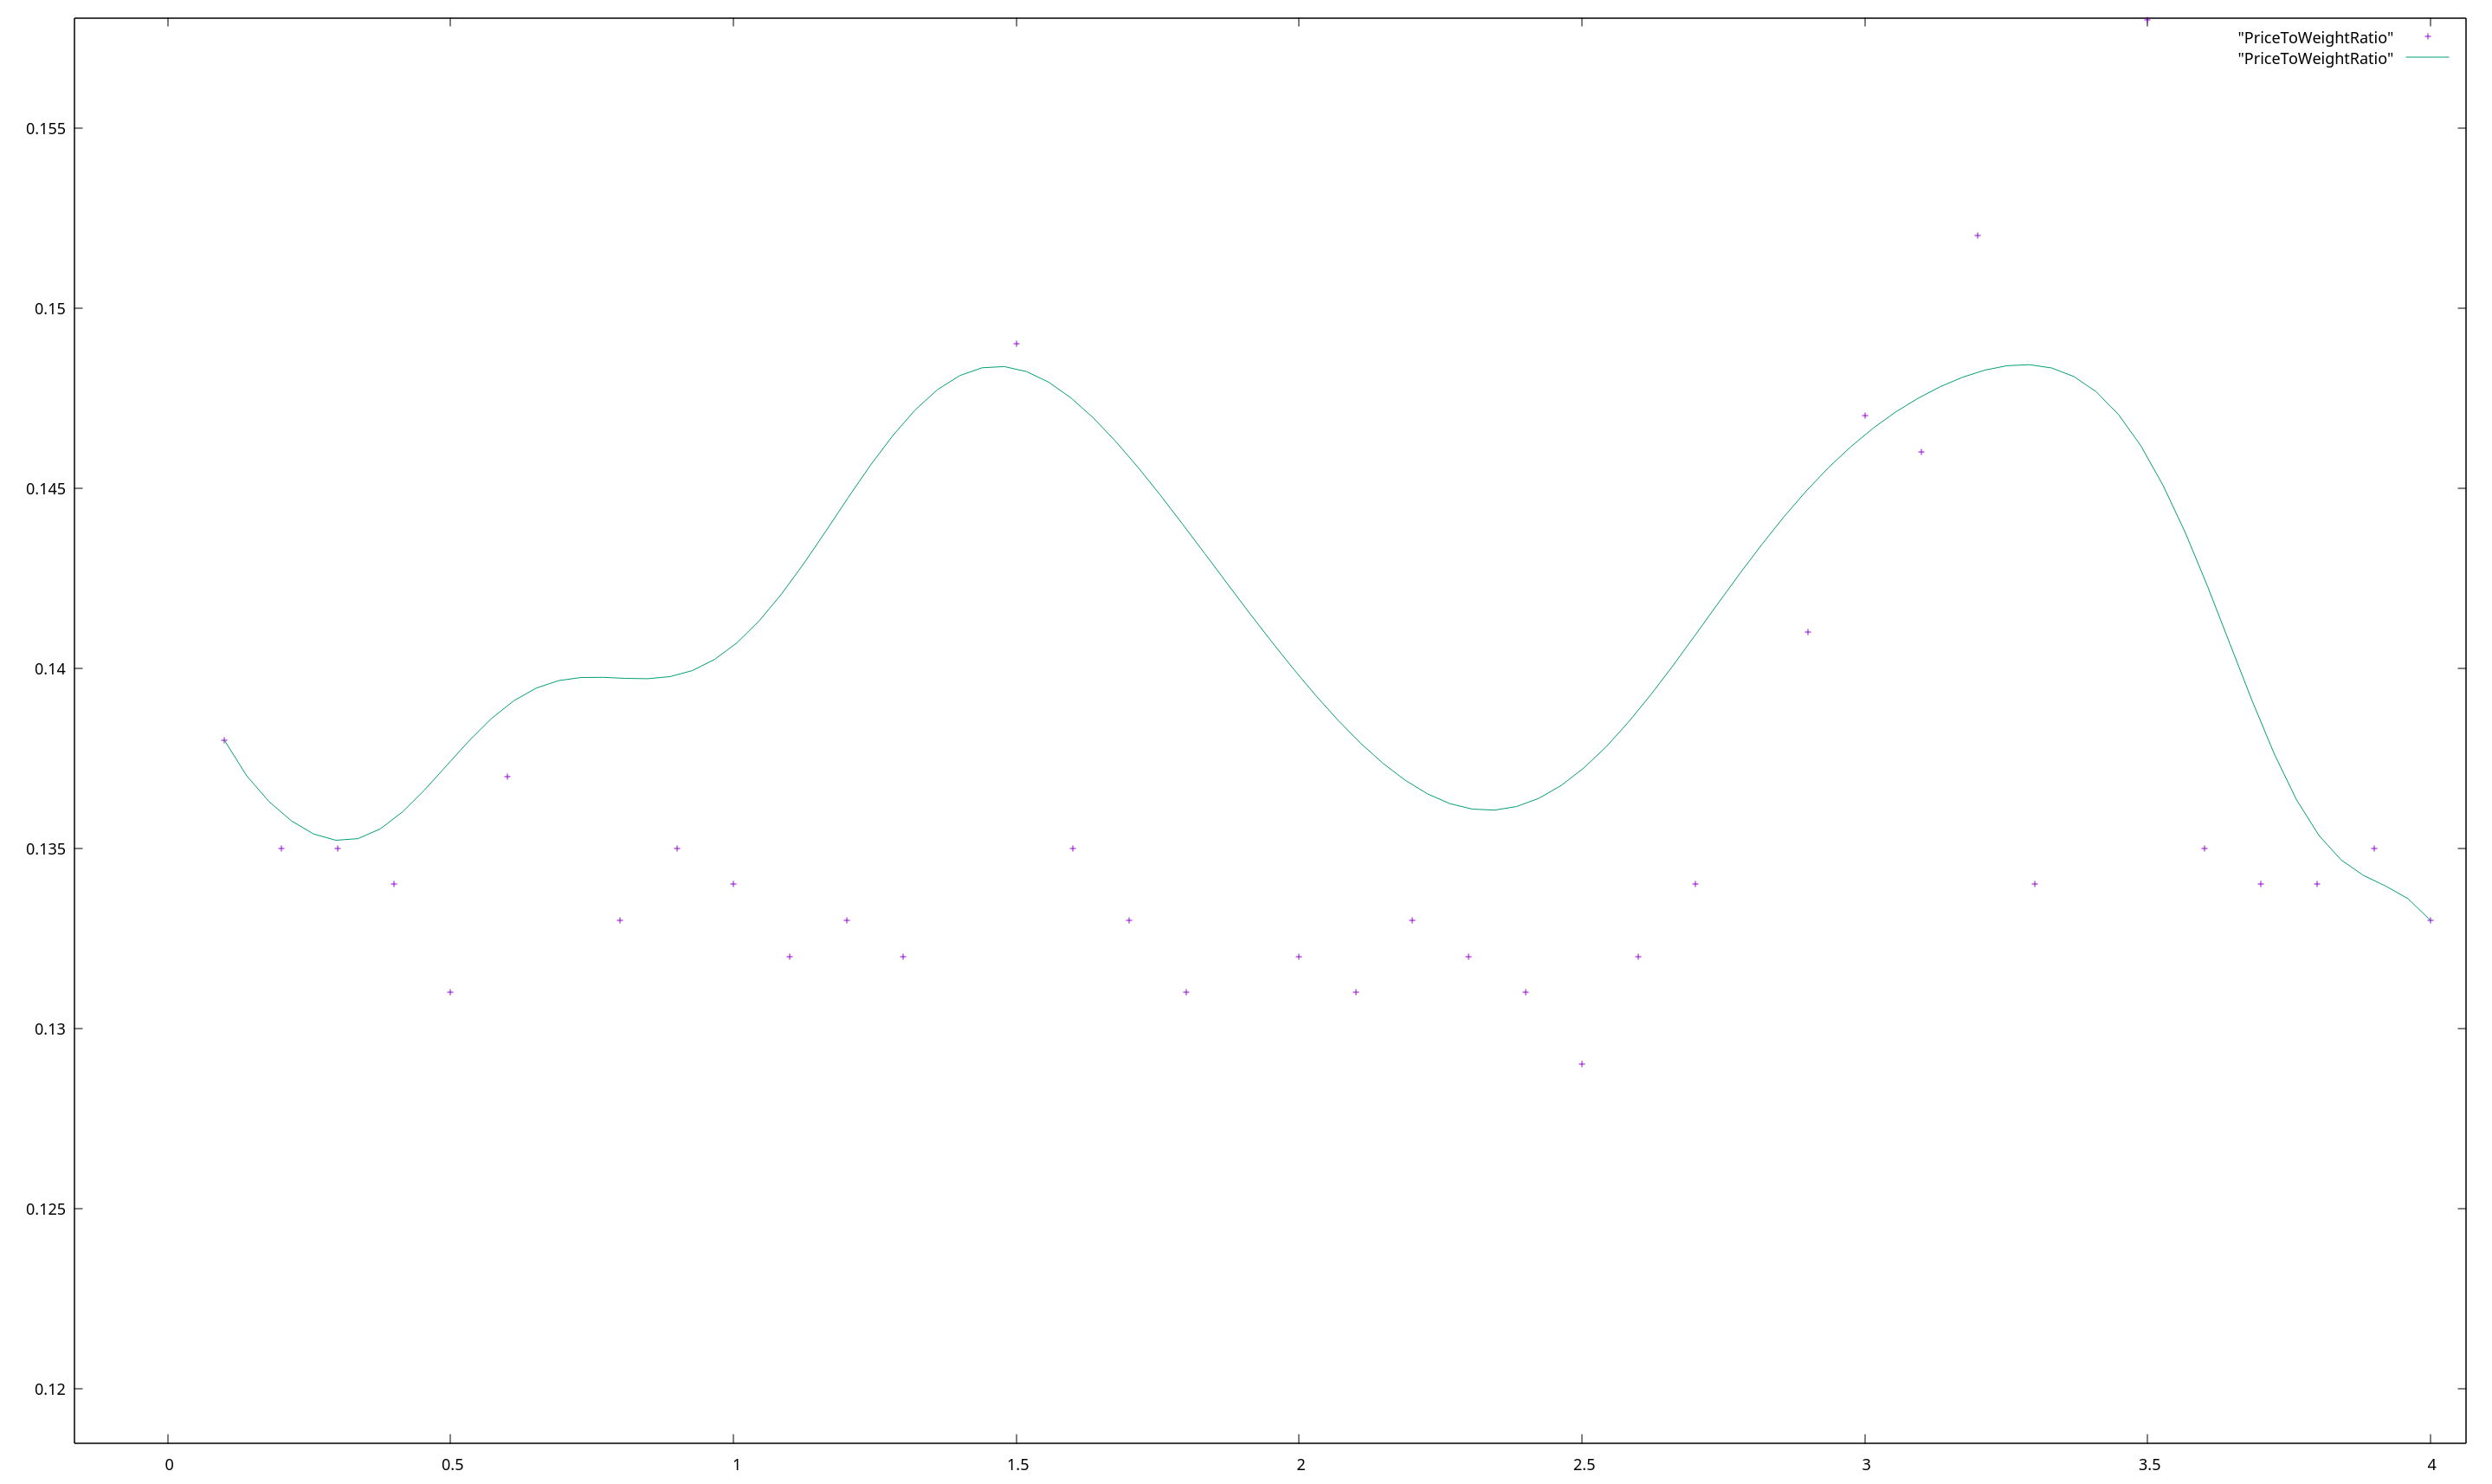
\includegraphics[width=\textwidth]{exp/big/PriceToWeightRatio}
\caption{Vývoj času výpočtu heuristikou (pro různý exponent, velké věci)}
\label{exp/big/PriceToWeightRatio}
\end{center}
\end{figure}

Graf \ref{exp/big/PriceToWeightRatio-relerrs} ale ukazuje závislost co se týče relativní chyby. Zdá se, že pro velkou převahu těžkých věcí se relativní chyba blíží nule. Heuristika rozhodující se pro věc s nejlepším poměrem ceny a váhy je tedy nejefektivnější, když jsou váhy co nejvyšší. 

\begin{figure}[H]
\begin{center}
\includegraphics[width=\textwidth]{exp/big/PriceToWeightRatio-relerrs}
\caption{Vývoj relativní chyby výpočtu heuristikou (pro různý exponent, velké věci)}
\label{exp/big/PriceToWeightRatio-relerrs}
\end{center}
\end{figure}

Srovnání těchto metod z hlediska výpočetního času je vidět v grafu \ref{exp/big/allExecTimes}. Z grafu je patrné, že žádná z metod není závislá na exponentu určujícím, jak velký důraz je kladen na výběr těžkých věcí. Jediná závislost se týká míry relativní chyby.

\begin{figure}[H]
\begin{center}
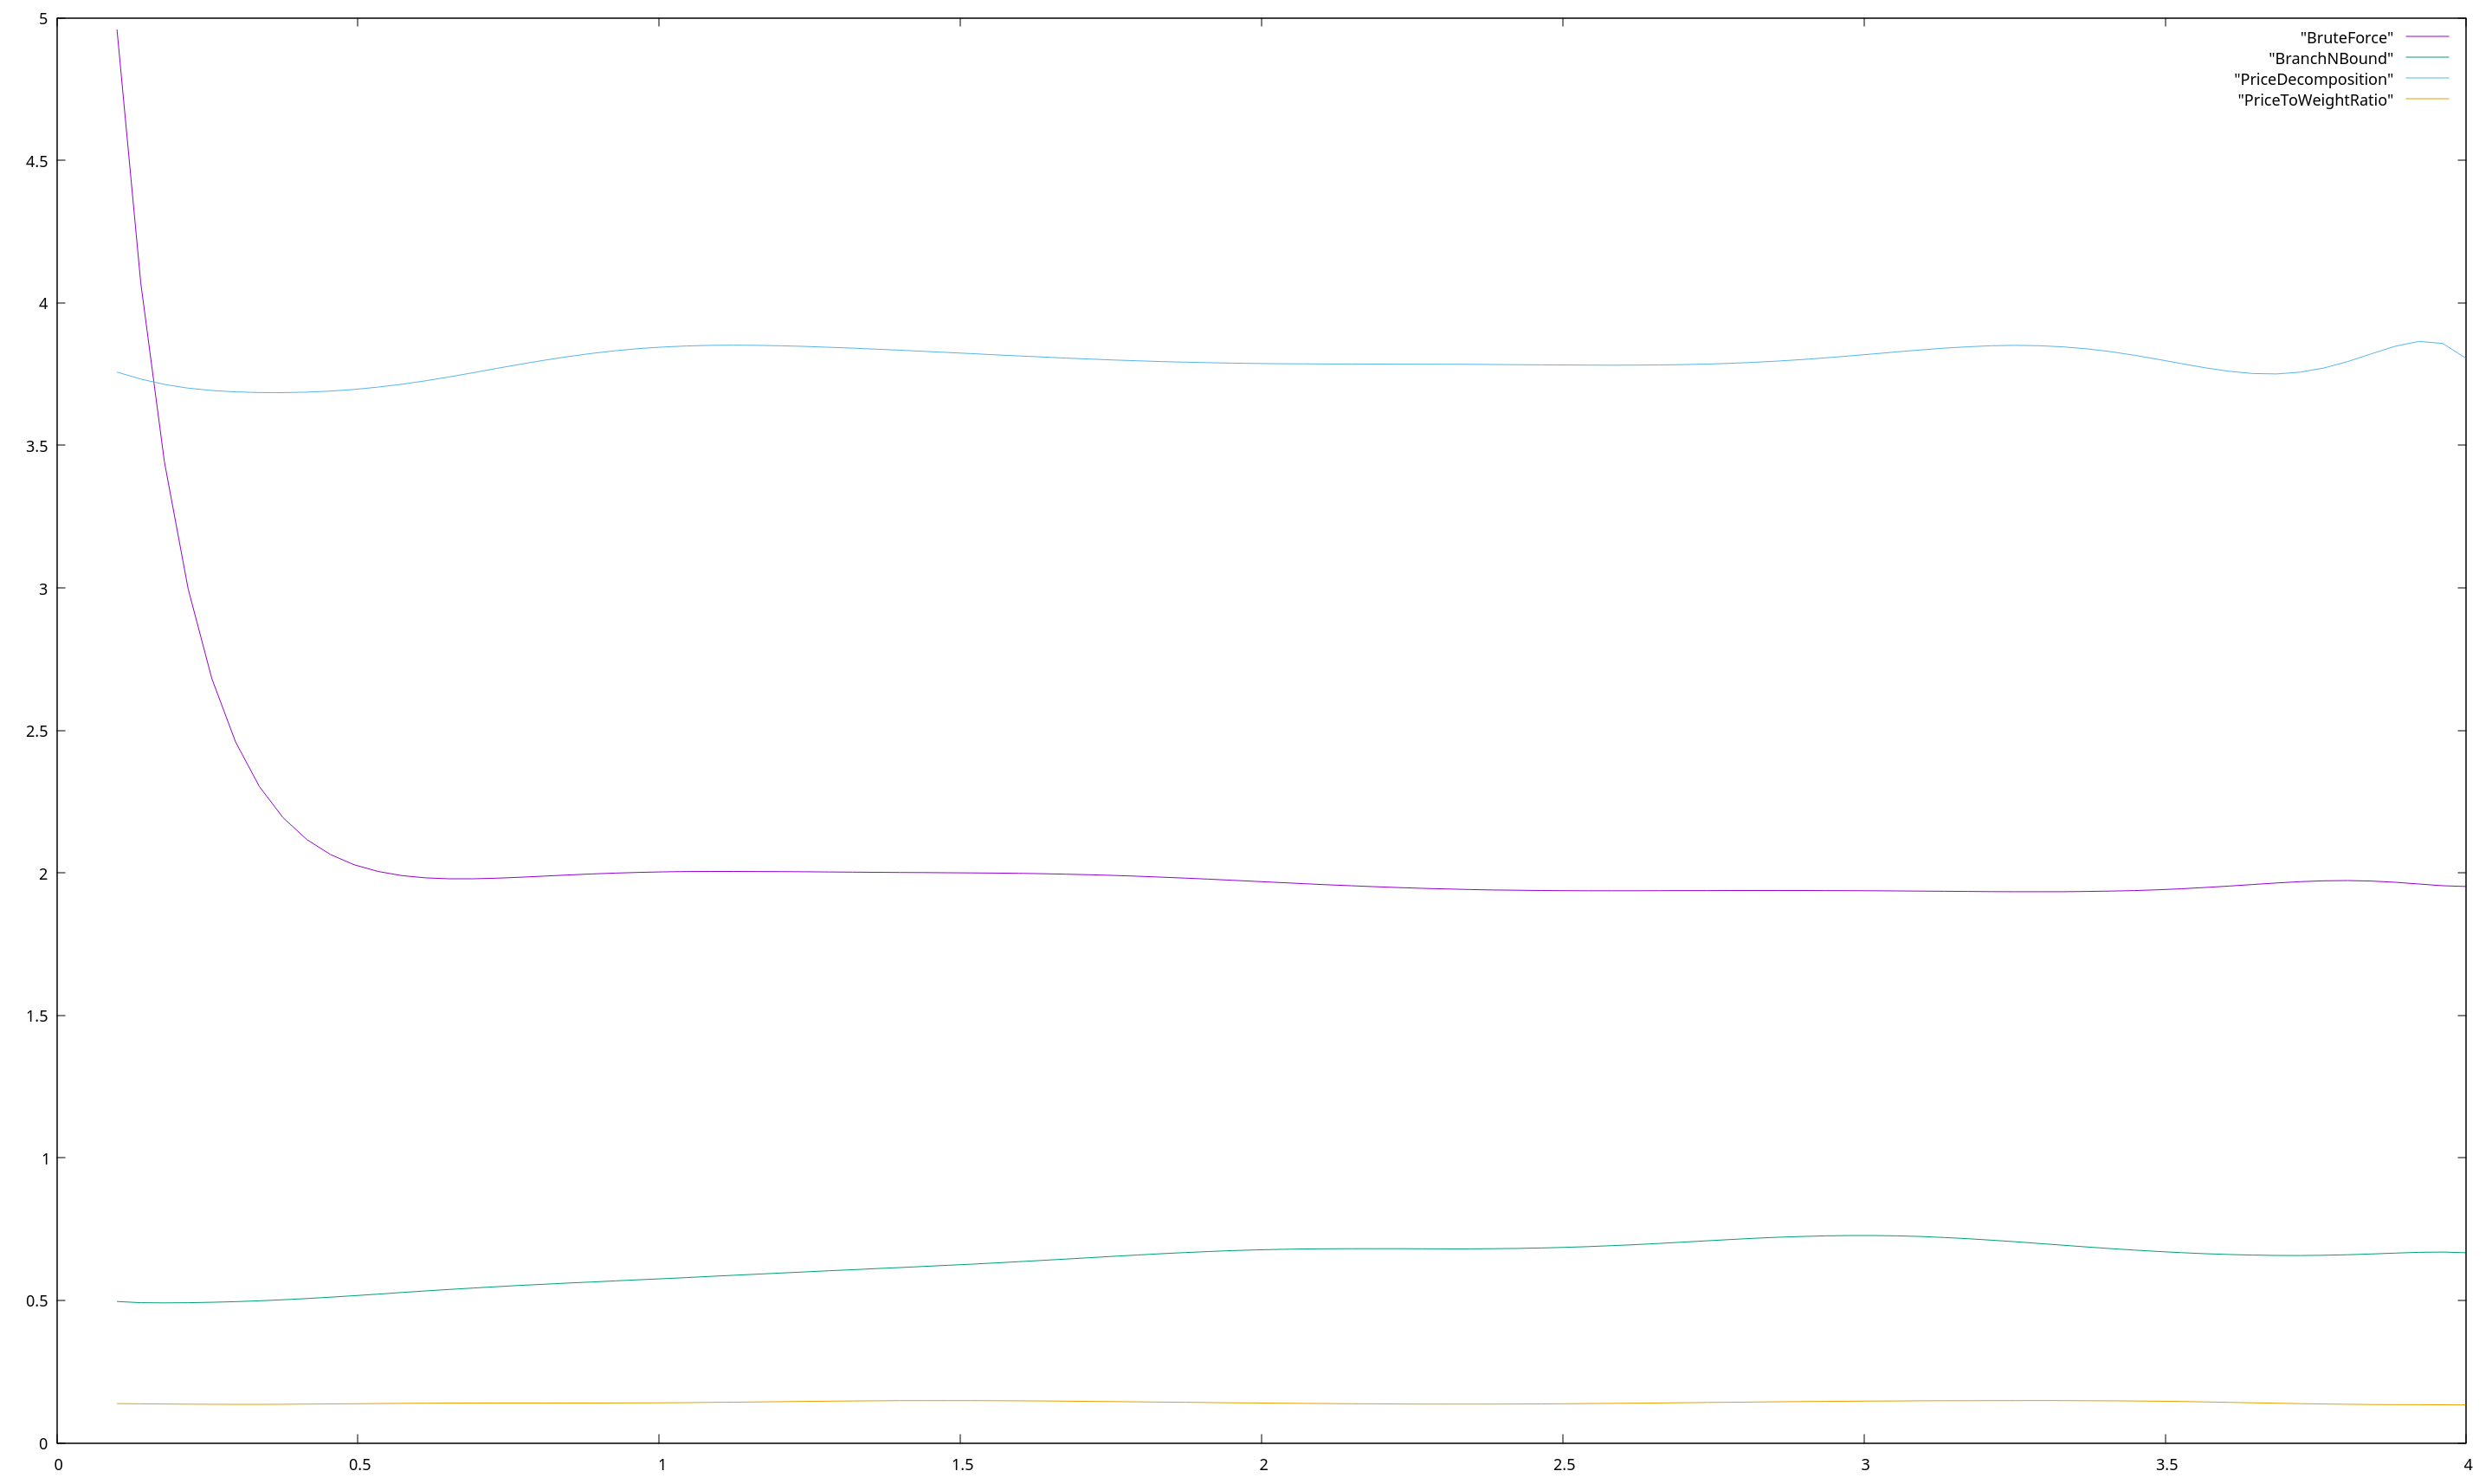
\includegraphics[width=\textwidth]{exp/big/allExecTimes}
\caption{Srovnání závislosti metod na exponentu určujícím převahu velkých věcí}
\label{exp/big/allExecTimes}
\end{center}
\end{figure}








\section{Závěr}

Zafixujeme-li parametry tak, jak je řečeno úvodu, jeví se obecně jako nejrychlejší jednoduchá heuristika, poté metoda větví a hranic, dále (s velkou mezerou) hrubá síla, a až na posledním místě dekompozice podle ceny. Důvodem, proč je dynamické programování pomalejší než hrubá síla, je skutečnost, že je maximální cena nastavena vysoko a velikost instance nízko. Obrovská výhoda dynamického programování by se projevila, jakmile bychom si vzal větší instance. Pak by efektivita této metody překročila ostatní exaktní. To však není předmětem této práce.

Vypozorovaných závislostí není mnoho. Nejviditelnější je závislost dekompozice podle ceny na maximální ceně. Měníme totiž parametr, na kterém je metoda přímo asymptoticky závislá. Další výraznou závislostí je závislost výpočetního času hrubé síly na poměru kapacity batohu ku sumární váze věcí. Zde se jedná o ořez při naplnění batohu, který se naplní tím později, čím je poměr větší. 

Relativní chyba jednoduché heuristiky založené na výběru nejlepšího poměru ceny a váhy klesá při větším poměru kapacity batohu ku sumární váze. Je to proto, že čím máme prostornější batoh, tím méně záleží na pořadí věcí, jak je do něj vkládáme. Dále relativní chyba klesá tehdy, když máme instanci problému, kde je velká převaha těžkých věcí.



\end{document}